\documentclass{article}


% if you need to pass options to natbib, use, e.g.:
\PassOptionsToPackage{numbers, compress}{natbib}


% to compile a camera-ready version, add the [final] option, e.g.:
\usepackage[final]{neurips_2024}



\usepackage[utf8]{inputenc} % allow utf-8 input
\usepackage[T1]{fontenc}    % use 8-bit T1 fonts
% \usepackage{hyperref}       % hyperlinks
\usepackage{url}            % simple URL typesetting
\usepackage{booktabs}       % professional-quality tables
\usepackage{amsfonts}       % blackboard math symbols
\usepackage{nicefrac}       % compact symbols for 1/2, etc.
\usepackage{microtype}      % microtypography
\usepackage{xcolor}         % colors
\usepackage{url}
\usepackage{graphicx}
\usepackage{animate}
\usepackage{listings}
\usepackage{algorithm}
\usepackage{algpseudocode}
\usepackage{enumitem}
\usepackage{silence}
\usepackage{makecell}
\usepackage{graphicx}  % For including images
\usepackage{wrapfig}   % For wrapping figures
% \usepackage{subfigure}
\usepackage{caption}
\usepackage{subcaption}
\usepackage{float}
\usepackage{multirow}
\hbadness=10000 \vbadness=10000 \vfuzz=30pt \hfuzz=30pt
\emergencystretch 1em

% \usepackage{fontspec}
% The "axessiblity" package can be found at: https://ctan.org/pkg/axessibility?lang=en
\usepackage[accsupp]{axessibility}  % Improves PDF readability for those with disabilities.
\newcommand{\nameofmethod}{HunyuanVideo}


\newcommand{\dq}[1]{\textcolor{cyan}{\bf\small [Daquan: #1]}}

\newcommand{\figref}[1]{Fig.~\ref{#1}}
\newcommand{\tabref}[1]{Tab.~\ref{#1}}
\newcommand{\eqnref}[1]{Eqn.~(\ref{#1})}
\newcommand{\secref}[1]{Sec.~\ref{#1}}
\newcommand{\myPara}[1]{\noindent\textbf{#1}}
\newcommand{\sArt}{state-of-the-art~}
\newcommand{\tabincell}[2]{\begin{tabular}{@{}#1@{}}#2\end{tabular}}
\newcommand{\para}[1]{\noindent\textbf{#1}}

\usepackage[pagebackref,breaklinks,colorlinks,citecolor=gray]{hyperref}


\title{\nameofmethod{}: A Systematic Framework For Large Video Generative Models}

\newcommand{\revist}[1]{\textcolor{red}{#1}}
\newcommand{\revisit}[2]{\textcolor{red}{#1(revisit: #2)}}

\begin{document}


\maketitle

\vspace{-20mm}
\begin{quote}
\vspace{-1mm}
\author{Hunyuan Foundation Model Team}
    ``\textit{Bridging the gap between closed-source and open-source video foundation models to accelerate community exploration.}'' \hfill --- \textbf{Hunyuan Foundation Model Team }
    % }
\vspace{-1mm}
\end{quote}


\begin{abstract}
Recent advancements in video generation have profoundly transformed daily life for individuals and industries alike. However, the leading video generation models remain closed-source, creating a substantial performance disparity in video generation capabilities between the industry and the public community. 
%
In this report, we present \nameofmethod{}, a novel open-source video foundation model that exhibits performance in video generation that is comparable to, if not superior to, leading closed-source models. \nameofmethod{} features a comprehensive framework that integrates several key contributions, including data curation, advanced architecture design, progressive model scaling and training, and an efficient infrastructure designed to facilitate large-scale model training and inference.
%
With those, we successfully trained a video generative model with over 13 billion parameters, making it the largest among all open-source models. 
%
We conducted extensive experiments and implemented a series of targeted designs to ensure high visual quality, motion dynamics, text-video alignment, and advanced filming techniques. According to professional human evaluation results, \nameofmethod{} outperforms previous state-of-the-art models, including Runway Gen-3, Luma 1.6, and 3 top performing Chinese video generative models. By releasing the code of the foundation model and its applications, we aim to bridge the gap between closed-source and open-source communities. This initiative will empower everyone in the community to experiment with their ideas, fostering a more dynamic and vibrant video generation ecosystem. The code is publicly available at \url{https://github.com/Tencent/HunyuanVideo}.
\end{abstract}

\begin{figure}[!h]
\vspace{-0.5cm}
    \centering
    \begin{minipage}[b]{0.3\textwidth}
        \centering
        \animategraphics[width=\textwidth]{24}{./videos/teaser/walking_woman/}{0}{24}
        % \caption{(a)}
    \end{minipage}%
    \hspace{0.01\textwidth} 
    \begin{minipage}[b]{0.5\textwidth}
        \centering
        \begin{minipage}[b]{0.48\textwidth}
            \centering
            \animategraphics[width=\textwidth]{30}{./videos/teaser/girl/}{52}{82}
            % \caption{(b)}
        \end{minipage}%
        \hspace{0.01\textwidth} % Space between the square videos
        \begin{minipage}[b]{0.48\textwidth}
            \centering

            \animategraphics[width=\textwidth]{20}{./videos/teaser/machine/}{42}{62}
            % \caption{(c))}
        \end{minipage}

        \vspace{0.01\textwidth} 

        \animategraphics[width=\textwidth]{24}{./videos/teaser/water_butterfly/}{52}{76}
        % \caption{(d)}
    \end{minipage}
    \caption{Non-curated multi-ratio generation samples with \nameofmethod{}, showing realistic, concept generalization and automatic scene-cut features.}
\end{figure}

\section{Introduction}
\label{sec:intro}

With extensive pre-training and advanced architectures, diffusion models~\cite{li2024hunyuandit,peebles2023scalable,esser2024scaling,rombach2022high,blattmann2023stable,girdhar2023emu,polyak2024movie,FLUX} have demonstrated superior performance in generating high-quality images and videos compared to previous generative adversarial network (GAN) methods \citep{brock2018large}.
However, unlike the image generation field, which has seen a proliferation of novel algorithms and applications across various open platforms, diffusion-based video generative models remain relatively inactive. We contend that one of the primary reasons for this stagnation is the lack of robust open-source foundation models as in T2I filed \cite{FLUX}. In contrast to the image generative model community, a significant gap has emerged between open-source and closed-source video generation models. Closed-source models tend to overshadow publicly available open-source alternatives, severely limiting the potential for algorithmic innovation from the public community. While the recent state-of-the-art model MovieGen \cite{polyak2024movie} has demonstrated promising performance, its milestone for open-source release has yet to be established.

\begin{figure}[h]
    \centering
    \begin{subfigure}[b]{0.47\textwidth}
        \centering
        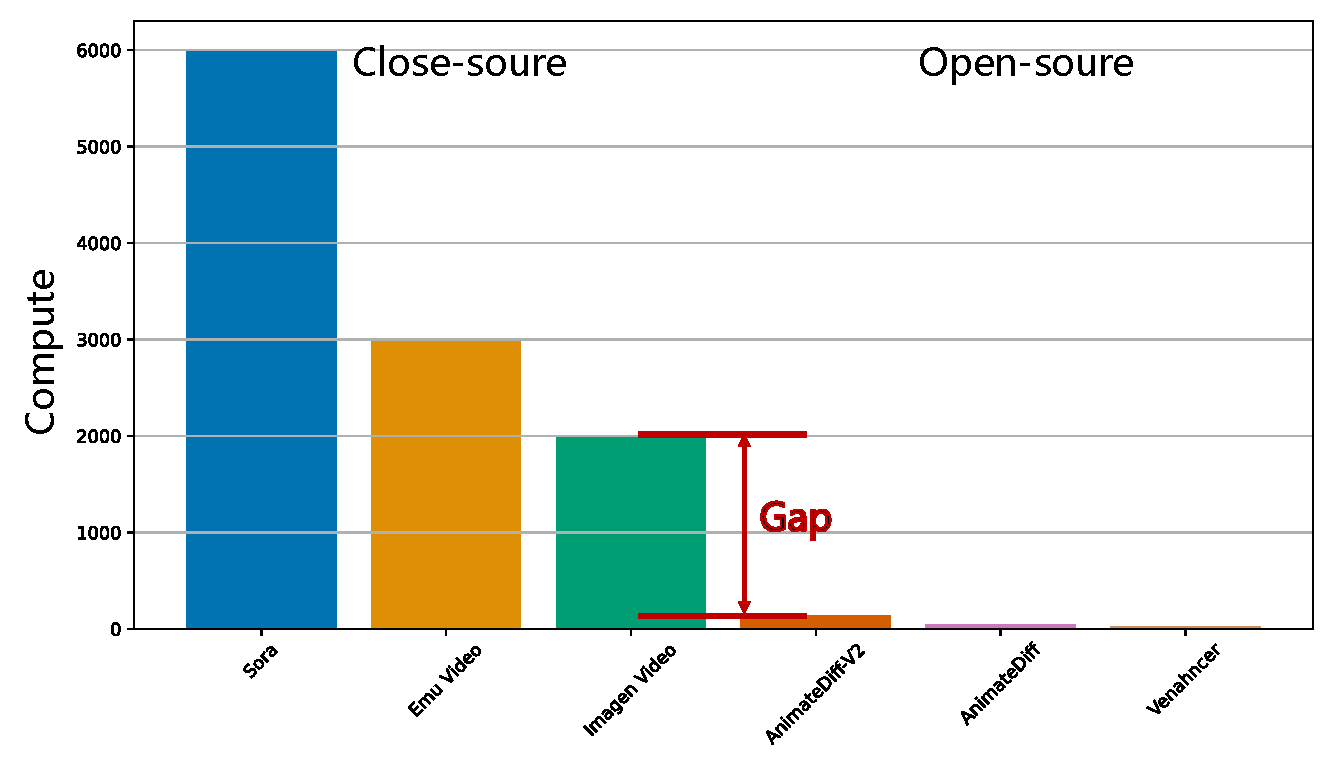
\includegraphics[width=\textwidth]{figures/compute_resource_v1.pdf} 
        % \caption{}
        % \label{fig:figure1}
    \end{subfigure}
    % \hspace{0.05\textwidth} 
    \begin{subfigure}[b]{0.45\textwidth}
        \centering
        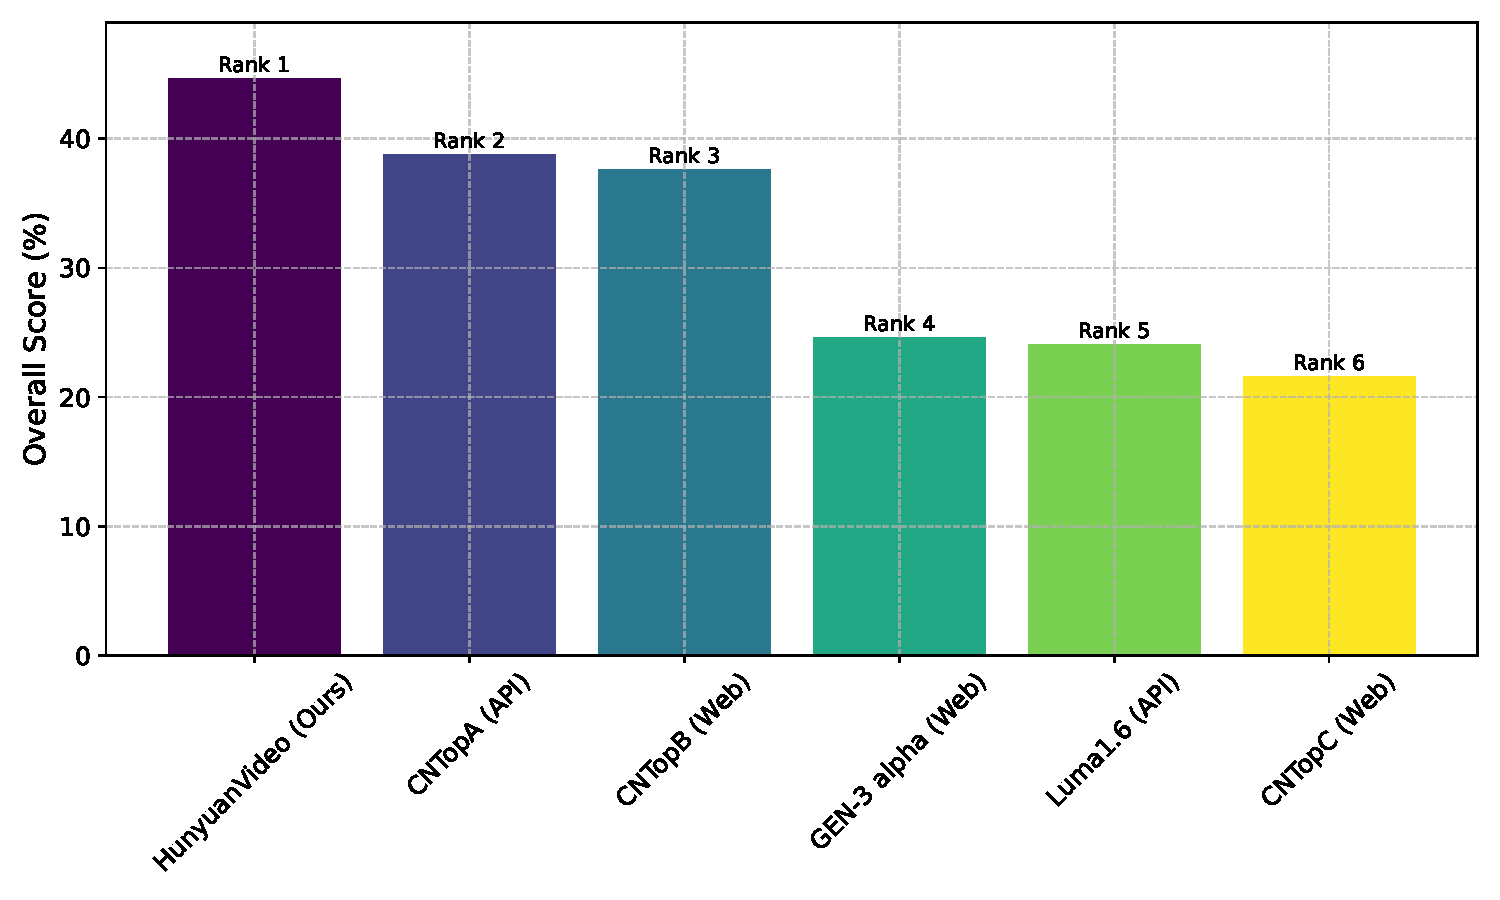
\includegraphics[width=\textwidth]{figures/ranking.pdf} 
        % \caption{}
        % \label{fig:figure2}
    \end{subfigure}
    \label{fig:side_by_side}
    \caption{Left: Computation resources used for closed-source and open-source video generation models. Right: Performance comparison between \nameofmethod{} and other selected strong baselines.}
\end{figure}

To address the existing gap and enhance the capabilities of the public community, this report presents our open-sourced foundational video generative model, \nameofmethod{}. This systematic framework encompasses training infrastructure, data curation, model architecture optimization, and model training.
%
Through our experiments, we discovered that randomly scaling the training data, computational resources, and model parameters of a simple Transformer-based generative model \cite{peebles2023scalable} trained with Flow Matching \cite{lipman2022flow} was not sufficiently efficient. Consequently, we explored an effective scaling strategy that can reduce computational resource requirements by up to 5× while achieving the desired model performance. With this optimal scaling approach and dedicated infrastructure, we successfully trained a large video model comprising 13 billion parameters, pre-training it on internet-scale images and videos.
%
After a dedicated progressive fine-tuning strategy, \nameofmethod{} excels in four critical aspects of video generation: visual quality, motion dynamics, video-text alignment, and semantic scene cut. We conducted a comprehensive comparison of \nameofmethod{} with leading global video generation models, including Gen-3 and Luma 1.6 and 3 top performing commercial models in China, using over 1,500 representative text prompts accessed by a group of 60 people. The results indicate that \nameofmethod{} achieves the highest overall satisfaction rates, particularly excelling in motion dynamics.


\section{Overview}
\label{sec:framework}
% \dq{Daquan, Weijie, Tianqi}
\nameofmethod{} is a comprehensive video training system encompassing all aspects from data processing to model deployment. This technical report is structured as follows:

\begin{itemize}
    \item In \textbf{Section \ref{sec:data}}, we introduce our data preprocessing techniques, including filtering and re-captioning models.
    \item \textbf{Section \ref{sec:model_arch}} presents detailed information about the architecture of all components of \nameofmethod{}, along with our training and inference strategies.
    \item In \textbf{Section \ref{sec:accelerate}}, we discuss methods for accelerating model training and inference, enabling the development of a large model with 13 billion parameters.
    \item \textbf{Section \ref{sec:exp}} evaluates the performance of our text-to-video foundation models and compares them with state-of-the-art video generation models, both open-source and proprietary.
    \item Finally, in \textbf{Section \ref{sec:application}}, we showcase various applications built on the pre-trained foundation model, accompanied by relevant visualizations as well as some video related functional models such as video to audio generative model.
\end{itemize}
\begin{figure}[h]
    \hfill
    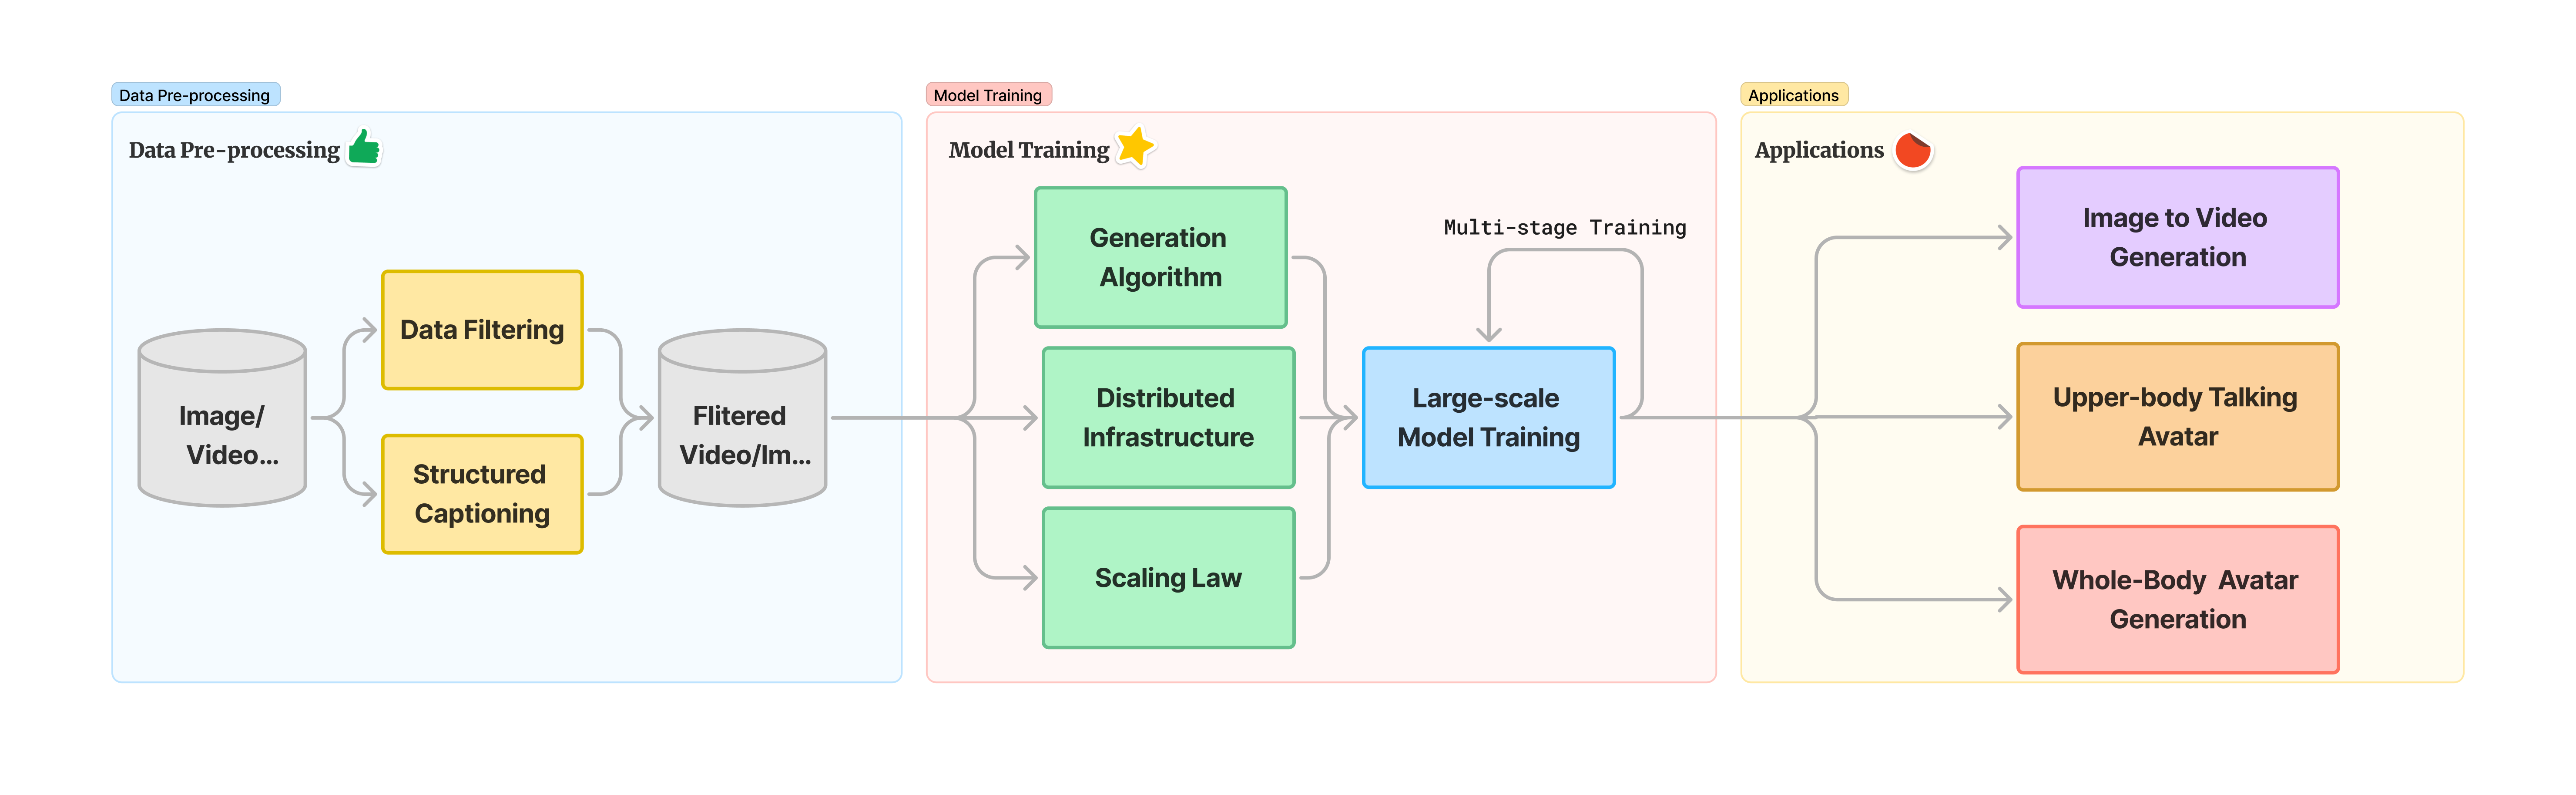
\includegraphics[width=\linewidth]{figures/overall.png}

    \caption{The overall training system for \nameofmethod{}.}
    \label{fig:pipeline_overview}
\end{figure}

% \section{Center Embedding Leads to The Hierarchical Rule}
\section{Data Complexity Determines Rule Preference}
\label{sec:data_complexity}

We find that models generalize hierarchically because they are trained on data which includes center embeddings, a linguistic structure which we describe in Section \ref{sec:center_embed}. Center-embedded sentences drive hierarchical generalization in both the QF task (Section \ref{sec:qf_result}) and the TI task (Section \ref{sec:ti_result}).

\begin{figure}[t!]
    \centering
    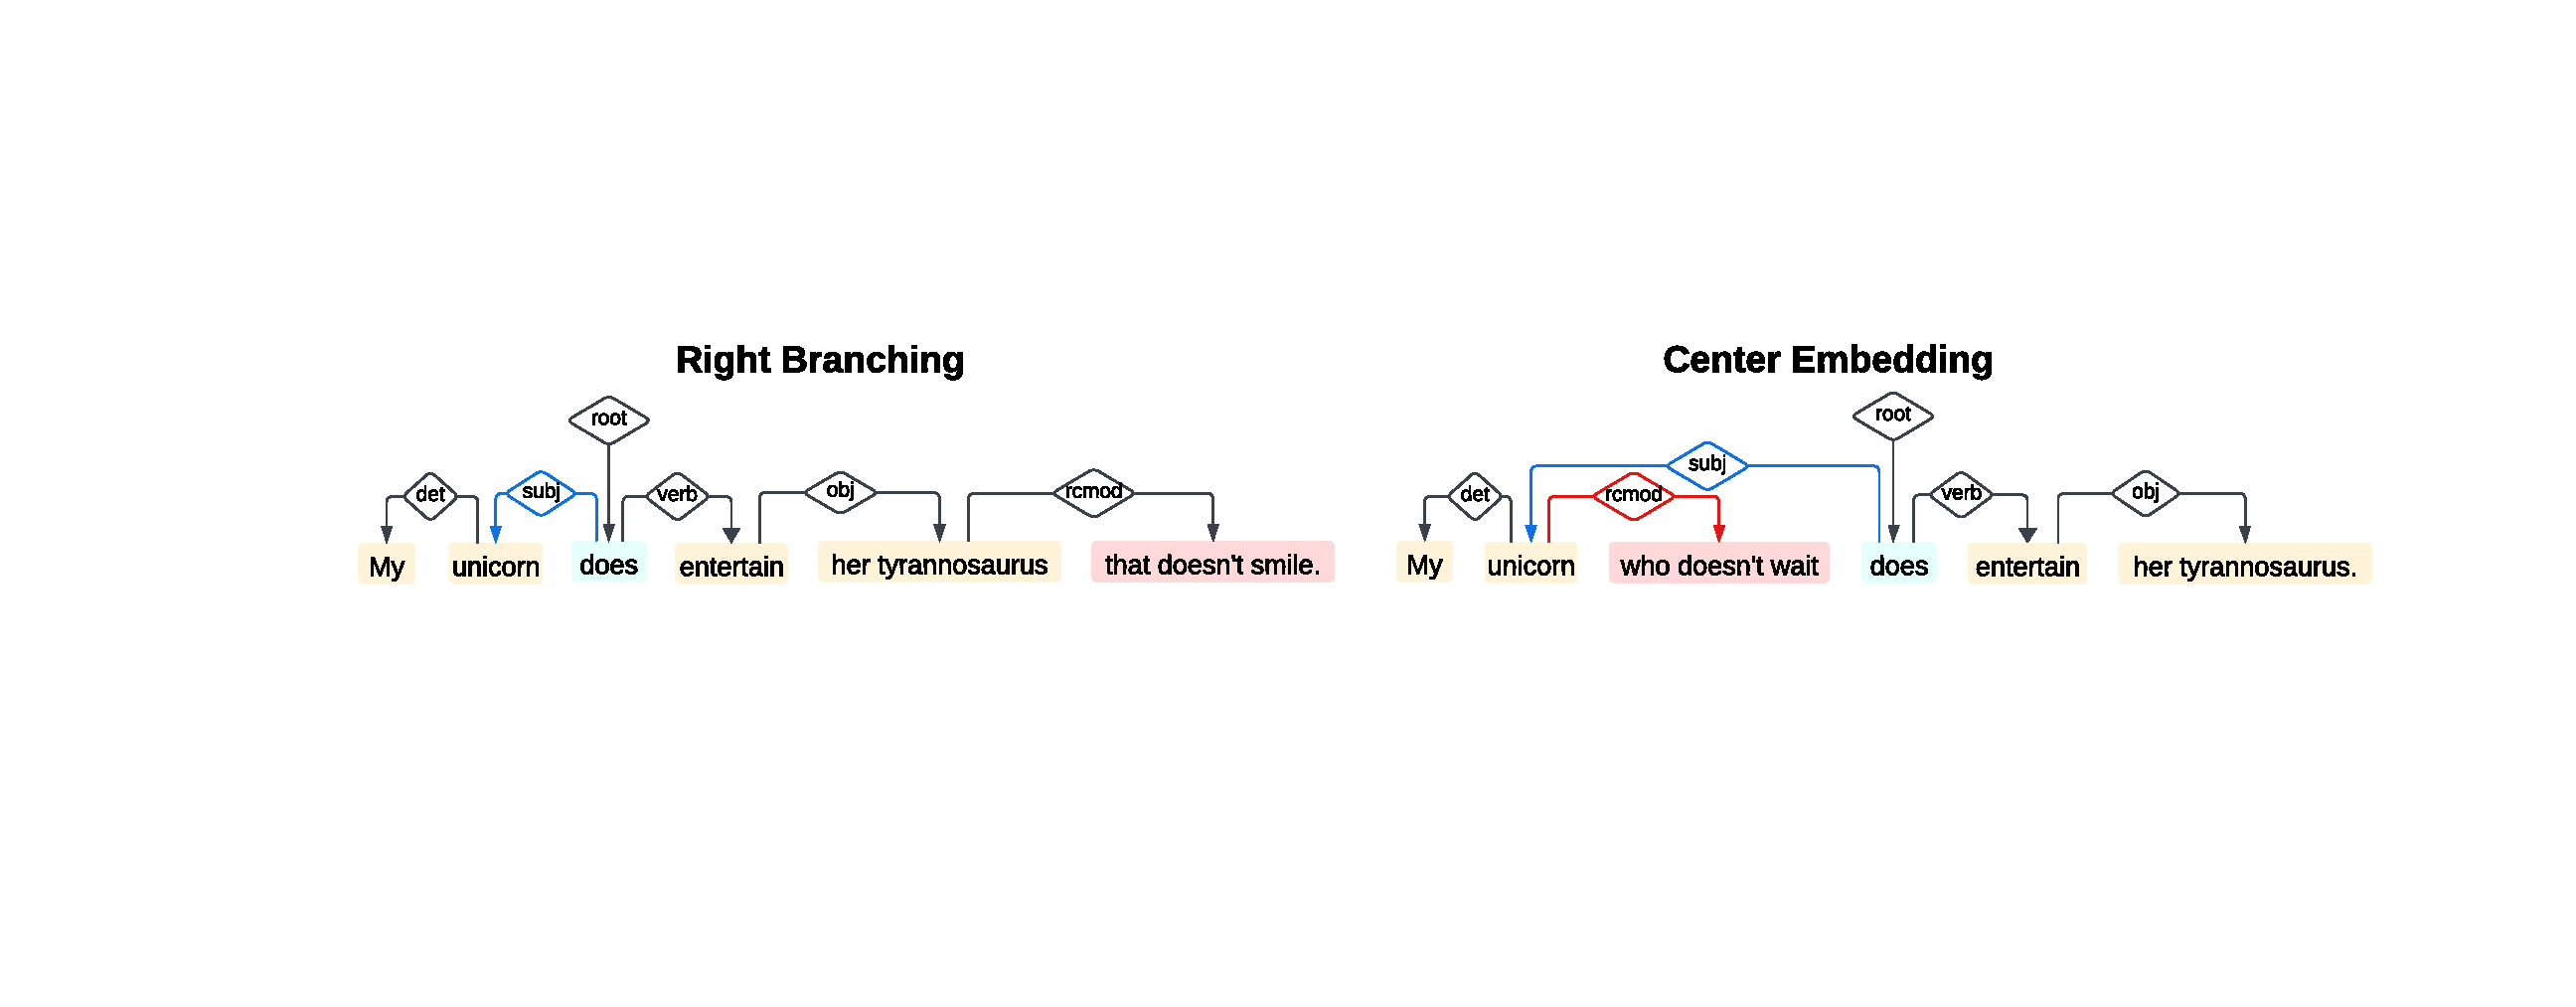
\includegraphics[width=1.0\textwidth]{figures/sentence_demo.pdf}
    \caption{\textbf{Sentence Examples.}   \textit{Left:} Right-branching sentence example. The linear progression of the main constituent is not interrupted by the relative clause. 
    \textit{Right:} Center-embedded sentence example. When the relative clause modifies the subject, it interrupts the linear progression of the main constituent. 
    }
    \label{fig:sentence_demo}
\end{figure}

\subsection{Center Embedding}
\label{sec:center_embed}
Center embedding occurs when a clause is placed recursively within another clause of the same type. Figure \ref{fig:sentence_demo} (\textit{left}) illustrates two examples of center-embedded sentences, where the embedded clause complicates syntactic parsing by placing an additional subject noun in between a verb and its own subject. Whereas center embeddings exhibit a recursive structure, sentences without center embeddings are exclusively right-branching. Right-branching structures may also include modifying clauses, but these clauses can only be appended at the end of the main clause, maintaining its linear flow (see Figure \ref{fig:sentence_demo}, \textit{right}). Linguists have long argued that center embeddings play a crucial role in grammar acquisition \citep{wexler1980formal} and give rise to tree-like syntactic structures \citep{Chomsky2015-bg}. 


We find that center embeddings, which are crucial for human language acquisition, also lead an LM to acquire hierarchical grammar rules. To correctly predict the next token, LMs must track syntactic connections between words in the context. In right-branching sentences, LMs can rely on linear proximity to identify these connections; as shown in Figure \ref{fig:sentence_demo}, a simple bigram model suffices to capture the subject-verb relationship for such sentences. In contrast, center embeddings introduce relative clauses of various lengths, making linear n-gram models inefficient for capturing subject-verb relationships. The recursive nature of the center embedding requires the model to track multiple subject-verb relationships: one for the main clause and a separate one for the embedded relative clause. In these cases, a tree structure is more efficient to model subject-verb relationships. 


\subsection{Question Formation Results}
\label{sec:qf_result}
As specified in Section \ref{sec:qf_task}, the training data for QF is ambiguous between the linear rule (i.e., moving the first auxiliary) and the hierarchical rule (i.e., moving the main auxiliary). Center-embedded sentences do not meet this ambiguity requirement and, therefore, cannot appear in question formation training samples. To ensure the model is exposed to diverse sentence types, \citet{McCoy2018-uv} introduced a secondary task to the QF training dataset: declaration copying. Like question formation, the declaration-copying example starts with a declarative sentence, but instead of transforming it, the model simply repeats it. Since the ambiguity requirement only applies to the primary question formation task, declaration-copying examples can include center embeddings. Concrete examples of both tasks can be found in Appendix \ref{appdx:data_sample}.


We train models on three modifications of the original training data, varying the composition of the declaration-copying subset. 
In \textit{Quest Only}, we remove all declaration-copying examples.
In \textit{Center embed}, we only keep center-embedded examples. In \textit{Right branch}, we only keep right-branching examples. 
Every modified training sets retains all examples of the primary task, question formation.
Every model trained, regardless of its training set composition, reaches 100\% in-distribution validation accuracy; however, the OOD generalization performance, shown in Figure \ref{fig:grokking_selection} (\textit{left}), differs significantly across the modified training sets. 

Our results confirm that declaration copying examples, specifically center embeddings, are essential for inducing hierarchical generalization.
Models trained without any declaration-copying examples fail to achieve an OOD accuracy above 75\%; so do models trained \textit{only} on right-branching  declaration-copying examples. When trained instead \textit{only} on center-embedded declaration-copying examples, models exhibit a strong preference for the hierarchical rule. This evidence suggests that center-embedded sentences direct a model towards the hierarchical rule. 

\begin{figure}[t!]
    \centering
    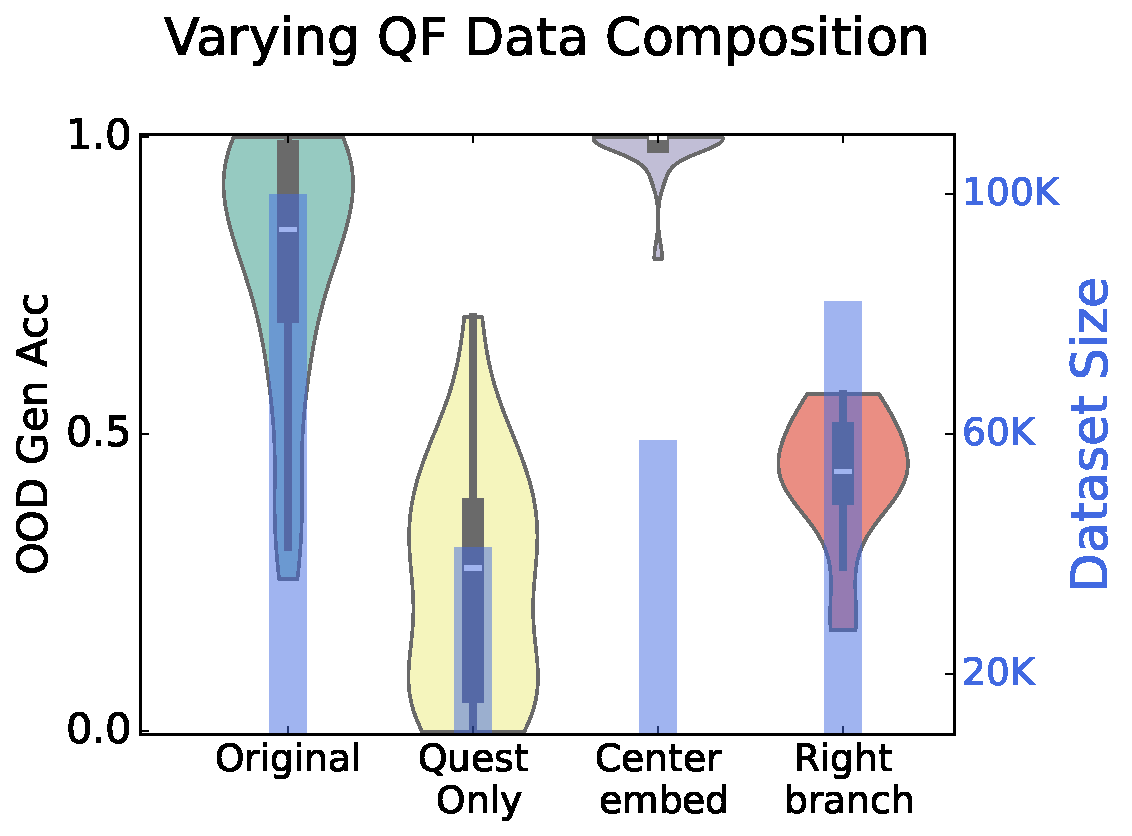
\includegraphics[width=0.41\linewidth]{figures/no_curriculum_main.pdf}
    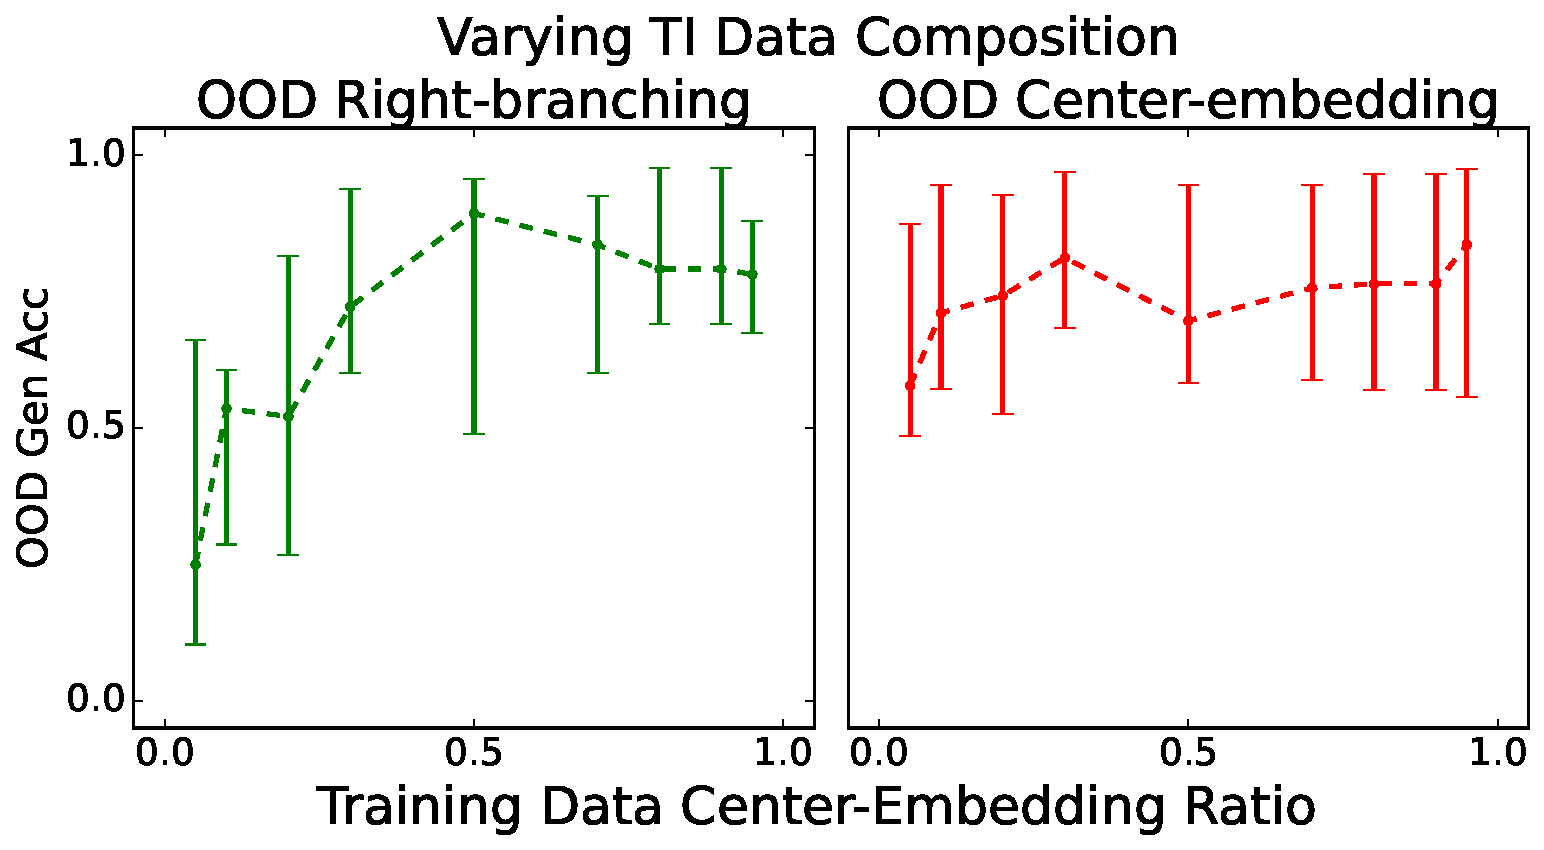
\includegraphics[width=0.55\linewidth]{figures/ti_simplicity_contamination.pdf}
    \caption{
    \textbf{Components of training data drive different generalization behaviors.} 
    \textit{Left:} Center-embedded sentences, which in the QF training data only appear in declaration copying examples, induce hierarchical generalization.
    \textit{Right:} Models are trained on different TI training data mixes and evaluated on two OOD sets: unambiguous right-branching sentences (\textit{green}) and unambiguous center-embedded sentences (\textit{red}). For center-embedded sentences, the hierarchical rule is preferred regardless of data mixes. For right-branching sentences, the model's preference for the hierarchical rule is exclusively driven by having a large mix of center-embedded sentences in the TI training data.}
    \label{fig:grokking_selection}
\end{figure}



\subsection{Tense Inflection Results}
\label{sec:ti_result}

In the TI training data, both right-branching and center-embedded sentences are made ambiguous by ensuring the distractor noun (i.e., a noun that appears between the main subject and the main verb) shares the same plurality as the main subject. For right-branching sentences, the distractor noun occurs in a prepositional phrase. For center-embedded sentences, the distractor noun occurs in a relative clause; either the subject or the object of the modifying clause can act as the distractor noun. We list examples below: 

\begin{enumerate}[itemsep=2pt,labelindent=10pt,topsep=0pt,parsep=0pt,partopsep=1pt, align=left, leftmargin=*]
    \item \textbf{Right Branching}: The noun in the prepositional phrase (e.g., `` \textit{to the cabinet}") acts as the distractor in the TI task.
    
    Example A (ID): \textit{The keys to the \textbf{cabinets} are on the table.}

    Example B (OOD): \textit{The keys to the \textbf{cabinet} are on the table.}
    
    \item \textbf{Center Embedding}: Either the subject or the object inside the relative clause acts as the distractor in the TI task.

    Example C (ID): \textit{The keys that unlock the \textbf{cabinets} are on the table.}

    Example D (OOD): \textit{The keys that unlock the \textbf{cabinet} are on the table.}
    
    
\end{enumerate}
We create variations of the TI training data by adjusting the ratio of right-branching to center-embedded samples while keeping the total training size constant.\footnote{The original training dataset contains a secondary past-tense copying task, to parallel the declaration-copying secondary task in QF. We show in Appendix \ref{appdx:ti_secondary} that the secondary task is not necessary, and we do not include it in our modified training sets.} A model's generalization behavior is tested on two OOD sets: one containing unambiguous right-branching sentences (e.g., Example B) and the other containing unambiguous center-embedded sentences (e.g., Example D). 

Generalization accuracies are shown in Figure \ref{fig:grokking_selection} (\textit{right}). When the training data is dominated by ambiguous right-branching sentences, the model fails to learn the hierarchical rule, as indicated by low OOD accuracy. However, when trained on a greater proportion of center-embedded sentences, the model systematically applies the hierarchical rule to both right-branching and center-embedded OOD sentences. As shown in Figure \ref{fig:grokking_selection} (\textit{right}), regardless of its training data mix, the model  generalizes hierarchically to OOD \textit{center embeddings}. In contrast, the model only generalizes hierarchically to \textit{right-branching sentences} after being exposed to a sufficient quantity of center-embedded sentences during training. In other words, the model eventually learns to treat non-recursive sequences as hierarchical through exposure to recursive center embeddings. These observations suggest that center embeddings drive the model's overall preference for tree structures. For further analysis of which center embedding structures induce this bias most efficiently, see Appendix \ref{appdx:obj_sbj_ctr_breakdown}.

% %%%%%%%%%%%%%%%%Previous version to preserve comments %%%%%%%%%%%%%%%%%%%%%%%%%%%%%%%%%%%%%%%%
% \iffalse
% \subsection{Tense Inflection} 
% \label{sec:ti_result}
% We now analyze hierarchical generalization in the tense inflection task, demonstrating the generality of our findings across grammatical rules. 
% The tense inflection setting from \citet{Linzen2016-vx} uses the same generation process as the question formation task, changing only the task itself.  
% This generation process leads to three types of sentences:

% \begin{enumerate}[itemsep=2pt,labelindent=10pt,topsep=0pt,parsep=0pt,partopsep=1pt, align=left, leftmargin=*]
%     \item The main verb immediately follows the subject noun.

%     Example: \textit{The keys are on the table.}
%     \item The main verb and the subject noun are separated by a prepositional phrase (e.g., `` \textit{to the cabinet}"). In all sentence examples, the prepositional phrase consistently follows the same syntactical structure and length (i.e., ``preposition $+$ determiner $+$ noun"). 

%     Example: \textit{The keys to the cabinet are on the table.}
%     \item The main verb and subject noun are separated by a relative clause, which can vary in syntactic composition and length.

%     Example: \textit{The keys that I used to unlock the cabinet are on the table.}
% \end{enumerate}


% By definition, both the first and second sentence types are right branching. In the second type, although a prepositional phrase is inserted within the main clause, it differs syntactically from a relative clause modifier. Unlike relative clause modifiers, prepositional phrases lack syntactic diversity, whereas relative clauses can exhibit the same of diversity as an entire sentence. In QF and TI data generated by CFG rules, a 4-gram model suffices to capture the subject-verb agreement. In contrast, relative clause modifiers (i.e., the third type) vary in both length and syntactic structure. All three sentence types are present in the original training data. Since sentences of the first type lack a distractor noun, they cannot be used to probe the model’s generalization, so the generalization set includes only the second and third types. As specified in Section \ref{sec:ti_task}, the TI training data only requires that the subject and distractor have the same plurality. Thus, center-embedded sentences can be included in the TI training data without violating the ambiguity requirement, and a secondary task is not necessary for TI.\footnote{In Appendix \ref{appdx:tense_tv}, we show that we can again leverage a secondary task such that a model trained on center-embedded tense inflection examples can generalize to right-branching sentences without having seen any examples of tense inflection on the sentence type, but not vice versa. }


% Our goal is to verify that center embeddings also drive OOD generalization in tense inflection. We create variations of the TI training data by adjusting the ratio of right-branching to center-embedded sentences, keeping the total training size constant. In Figure \ref{fig:ti_selection}, we report the model's OOD behavior across two data partitions. Figure \ref{fig:ti_selection} (\textit{left}) shows the model's generalization accuracy on unambiguous right-branching sentences when trained on different data mixes. When training data is dominated by ambiguous right-branching sentences, the model fails to learn the hierarchical rule, as indicated by low OOD generalization accuracy. However, as we increase the proportion of center-embedded sentences, these sentences---despite being ambiguous---bias the model towards the hierarchical rule, reflected by improved generalization accuracy.

% Figure \ref{fig:ti_selection} (\textit{right}) shows that the model consistently prefers the hierarchical rule for center-embedded sentences, regardless of data composition. These results indicate that the model’s preference for the hierarchical rule is primarily driven by center-embedded sentences. Moreover, with a high proportion of center-embedded sentences in the training data, this hierarchical rule preference extends to right-branching sentences as well.


% \fi

\section{Model Architecture Design}
The overview of our \nameofmethod{} model is shown in Fig.~\ref{fig:hunyuanvideo_overview}. This section describes the Causal 3D VAE, diffusion backbone, and scaling laws experiments.

\label{sec:model_arch}
\begin{figure}[t]
    \centering
    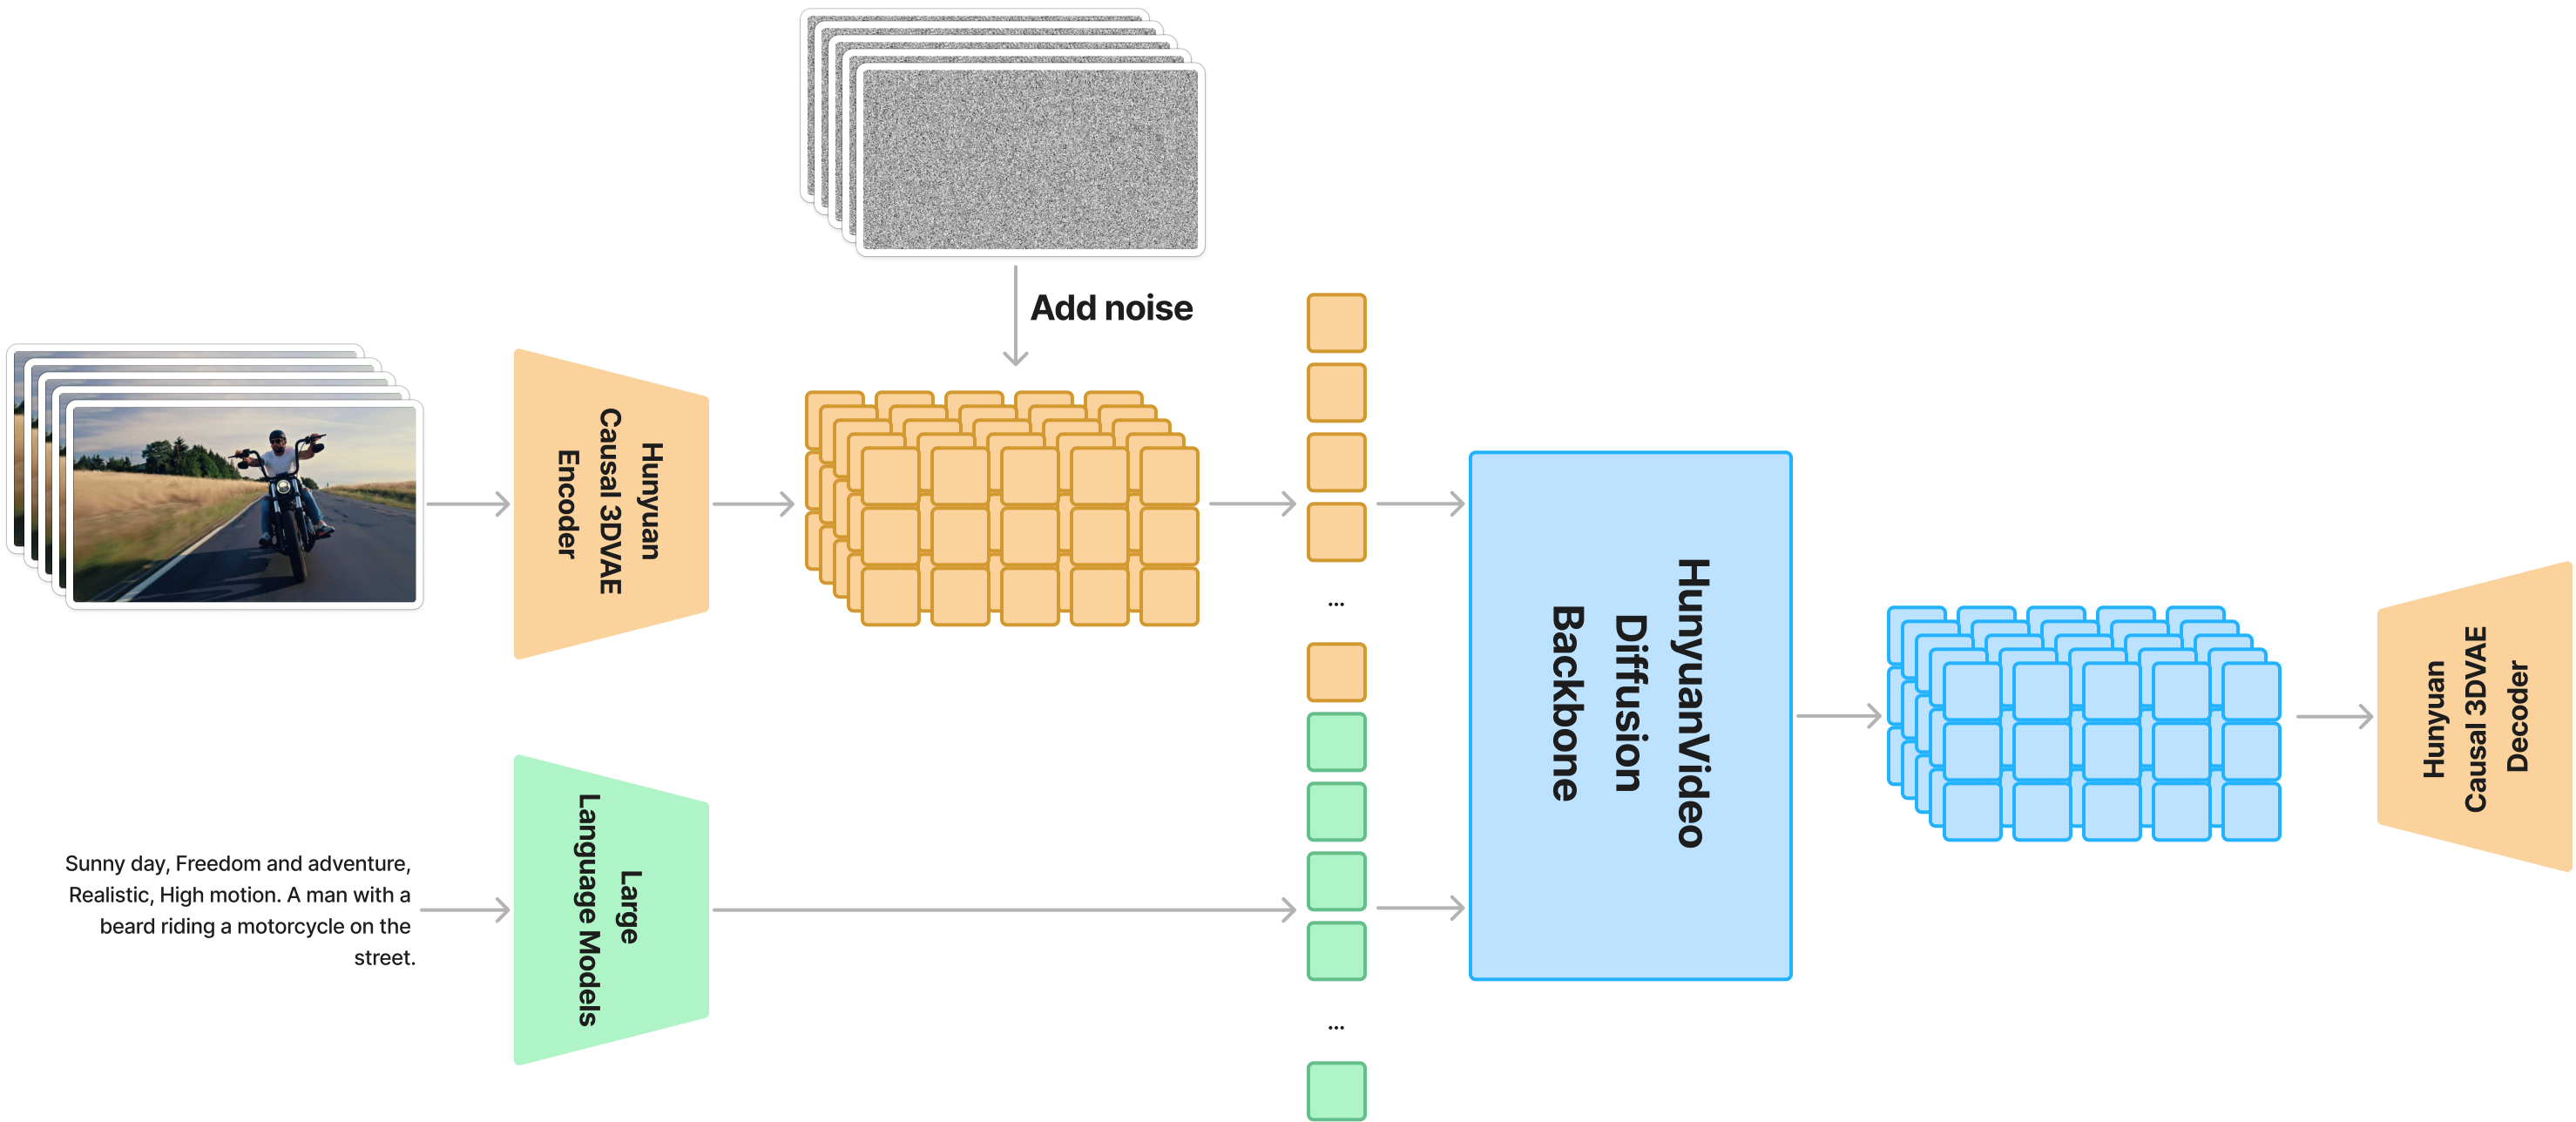
\includegraphics[width=0.95\linewidth]{figures/hunyuanvideo_overview.png}

    \caption{The overall architecture of \nameofmethod{}. The model is trained on a spatial-temporally compressed latent space, which is compressed through Causal 3D VAE. Text prompts are encoded using a large language model, and used as the condition. Gaussian noise and condition are taken as input, our model generates a output latent, which is decoded into images or videos through the 3D VAE decoder.}
    \label{fig:hunyuanvideo_overview}
\end{figure}

% \dq{add in architecture design of 3D VAE and DiT. Put diagram here also.}
\subsection{3D Variational Auto-encoder Design}\label{3dVAE}

Similar to previous work~\cite{polyak2024movie,yang2024cogvideox}, we train a 3DVAE to compress pixel-space videos and images into a compact latent space. To handle both videos and images, we adopt CausalConv3D~\cite{yu2023language}. For a video of shape $(T+1) \times 3 \times H \times W$, our 3DVAE compresses it into latent features with shape $(\frac{T}{c_t} + 1) \times C \times (\frac{H}{c_s}) \times (\frac{W}{c_s})$. In our implementation, $c_t=4$, $c_s=8$, and $C=16$. This compression significantly reduces the number of tokens for the subsequent diffusion transformer model, allowing us to train videos at the original resolution and frame rate. The model structure is illustrated in Figure \ref{fig:vae-model-arch}.

\begin{figure}[t]
    \centering
    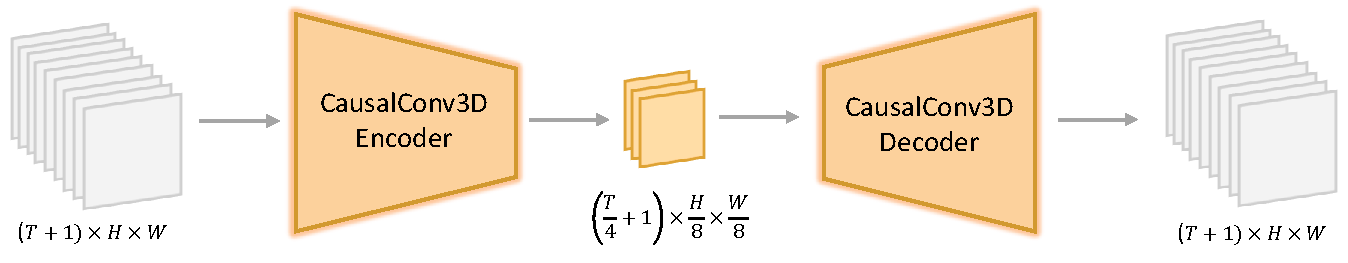
\includegraphics[width=0.95\linewidth]{figures/vae-model-arch.pdf}
    \caption{ The architecture of our 3DVAE.}
    \label{fig:vae-model-arch}
\end{figure}

\subsubsection{Training}
In contrast to most previous work \cite{polyak2024movie,chen2024od,zhou2024allegro}, we do not rely on a pre-trained image VAE for parameter initialization; instead, we train our model from scratch. 
To balance the reconstruction quality of videos and images, we mix video and image data at a ratio of $4:1$. Besides the routinely used $L_1$ reconstruction loss and KL loss $L_{kl}$, we also incorporate perceptual loss $L_{lpips}$ and GAN adversarial loss $L_{adv}$ \cite{esser2021taming} to enhance the reconstruction quality. The complete loss function is shown in Equation \ref{eq:vae-loss}.

\begin{equation}
    \label{eq:vae-loss}
    \text{Loss} = L_{1} + 0.1 L_{lpips} + 0.05 L_{adv} + 10^{-6} L_{kl}
\end{equation}

During training, we employ a curriculum learning strategy, gradually training from low-resolution short video to high-resolution long video. To improve the reconstruction of high-motion videos, we randomly choose a sampling interval from the range $1 \sim 8$ to sample frames evenly across video clips.

\subsubsection{Inference}
Encoding and decoding high-resolution long videos on a single GPU can lead to out-of-memory (OOM) errors. To address this, we use a spatial-temporal tiling strategy, splitting the input video into overlapping tiles along the spatial and temporal dimensions. Each tile is encoded/decoded separately, and the outputs are stitched together. For the overlapping regions, we utilize a linear combination for blending. This tiling strategy allows us to encode/decode videos in arbitrary resolutions and durations on a single GPU.

We observed that directly using the tiling strategy during inference can result in visible artifacts due to inconsistencies between training and inference. To solve this, we introduce an additional finetuning phase where the tiling strategy is randomly enabled/disabled during training. This ensures the model is compatible with both tiling and non-tiling strategies, maintaining consistency between training and inference. 

\begin{figure}[ht]
    \centering
    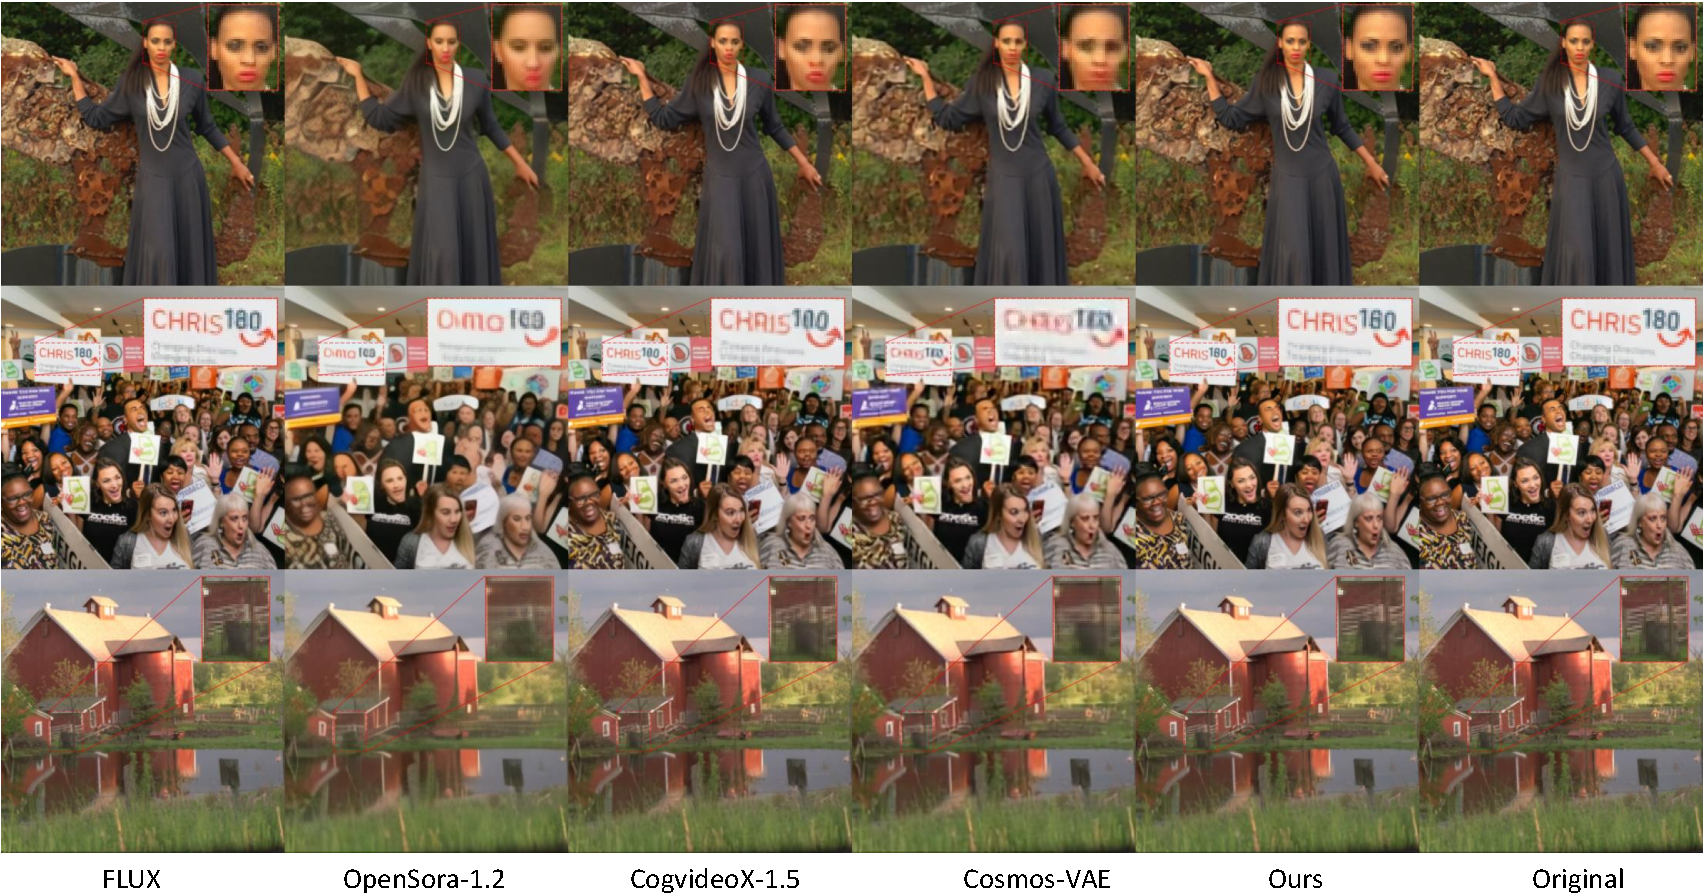
\includegraphics[width=\linewidth]{figures/vae-sota-cmp.pdf}
    \caption{VAE reconstruction case comparison.}
    \label{fig:vae-sota-cmp}
\end{figure}

Table \ref{tab:sota_vae} compares our VAE with open-source state-of-the-art VAEs. On video data, our VAE demonstrates a significantly higher PSNR compared to other video VAEs. On images, our performance surpasses both video VAEs and image VAE. Figure \ref{fig:vae-sota-cmp} shows several cases at $256 \times 256$ resolution. Our VAE demonstrates significant advantages in text, small faces, and complex textures.
%Table \ref{tab:sota_vae} compares our VAE with open-source state-of-the-art VAEs. On video data, our VAE demonstrates a significantly higher PSNR compared to other video VAEs, achieving performance comparable to frame-wise image VAE while maintaining a 4x higher temporal compression. On images, our PSNR not only surpasses that of other video VAEs but also exceeds that of image VAE. Figure \ref{fig:vae-sota-cmp} shows several cases at $256 \times 256$ resolution. It is evident that our VAE demonstrates significant advantages in  text, small faces, and complex textures.


\begin{table*}[ht]
\renewcommand{\arraystretch}{1.2}
\small
\centering  
\caption{VAE reconstruction metrics comparison.}
\begin{tabular}{lcccc}
\toprule
\multirow{2}{*}{Model} & Downsample  & \multirow{2}{*}{$|z|$} & ImageNet (256$\times$256)
& MCL-JCV (33$\times$360$\times$640) \\
& Factor & & PSNR$\uparrow$ & PSNR$\uparrow$ \\
\midrule
%FLUX-VAE~\cite{FLUX}                   & $1 \times 8 \times 8$ & 16 & 32.70 & 37.87 \\
FLUX-VAE~\cite{FLUX}                   & $1 \times 8 \times 8$ & 16 & 32.70 & - \\
\midrule
OpenSora-1.2~\cite{opensora}           & $4 \times 8 \times 8$ & 4  & 28.11 & 30.15 \\
CogvideoX-1.5~\cite{yang2024cogvideox} & $4 \times 8 \times 8$ & 16 & 31.73 & 33.22 \\
Cosmos-VAE~\cite{cosmos}               & $4 \times 8 \times 8$ & 16 & 30.07 & 32.76 \\
Ours                                   & $4 \times 8 \times 8$ & 16 & 33.14 & 35.39 \\
\bottomrule
\end{tabular}
\label{tab:sota_vae}
\end{table*}

% \dq{@Common Utility Team}

\subsection{Unified Image and Video Generative Architecture}
\label{sec:architecture}
% \dq{@Weijie, Tianqi, Zijian, Jianwei}

% In this section, we introduce the Transformer design in \nameofmethod{}. We adopt a unified Full Attention mechanism, primarily based on the following three reasons:
% Firstly, it has been validated to exhibit superior performance compared to divided spatiotemporal attention.
% Secondly, it supports unified generation for both images and videos, simplifying the training process while facilitating better model scalability.
% Lastly, it leverages existing LLM-related acceleration capabilities more effectively, enhancing both model training and inference efficiency.

% For a given video-text pair, the model is performed within the 3D latent space mentioned in section \ref{3dVAE}.  More specifically, for the video branch, the input is first compressed into latents of shape $T\times C \times H \times W$. We treat images as single-frame videos, to unify the input processing. These latents are then patchified and unfolded into a 1D sequence of tokens with a length of $\frac{T}{k_t}\cdot \frac{H}{k_h}\cdot \frac{W}{k_w}$, using a 3D convolution with a kernel size of $k_t\times k_h\times k_w$.  For the text branch, we first employ an advanced LLM to encode it into a text embedding sequence, which contains fine-grained semantics information. Meanwhile, we use the CLIP model to extract pooled text representation, which contains global information, which are added to the timestep embedding after dimensionality expansion.
\begin{figure}[ht]
    \centering
    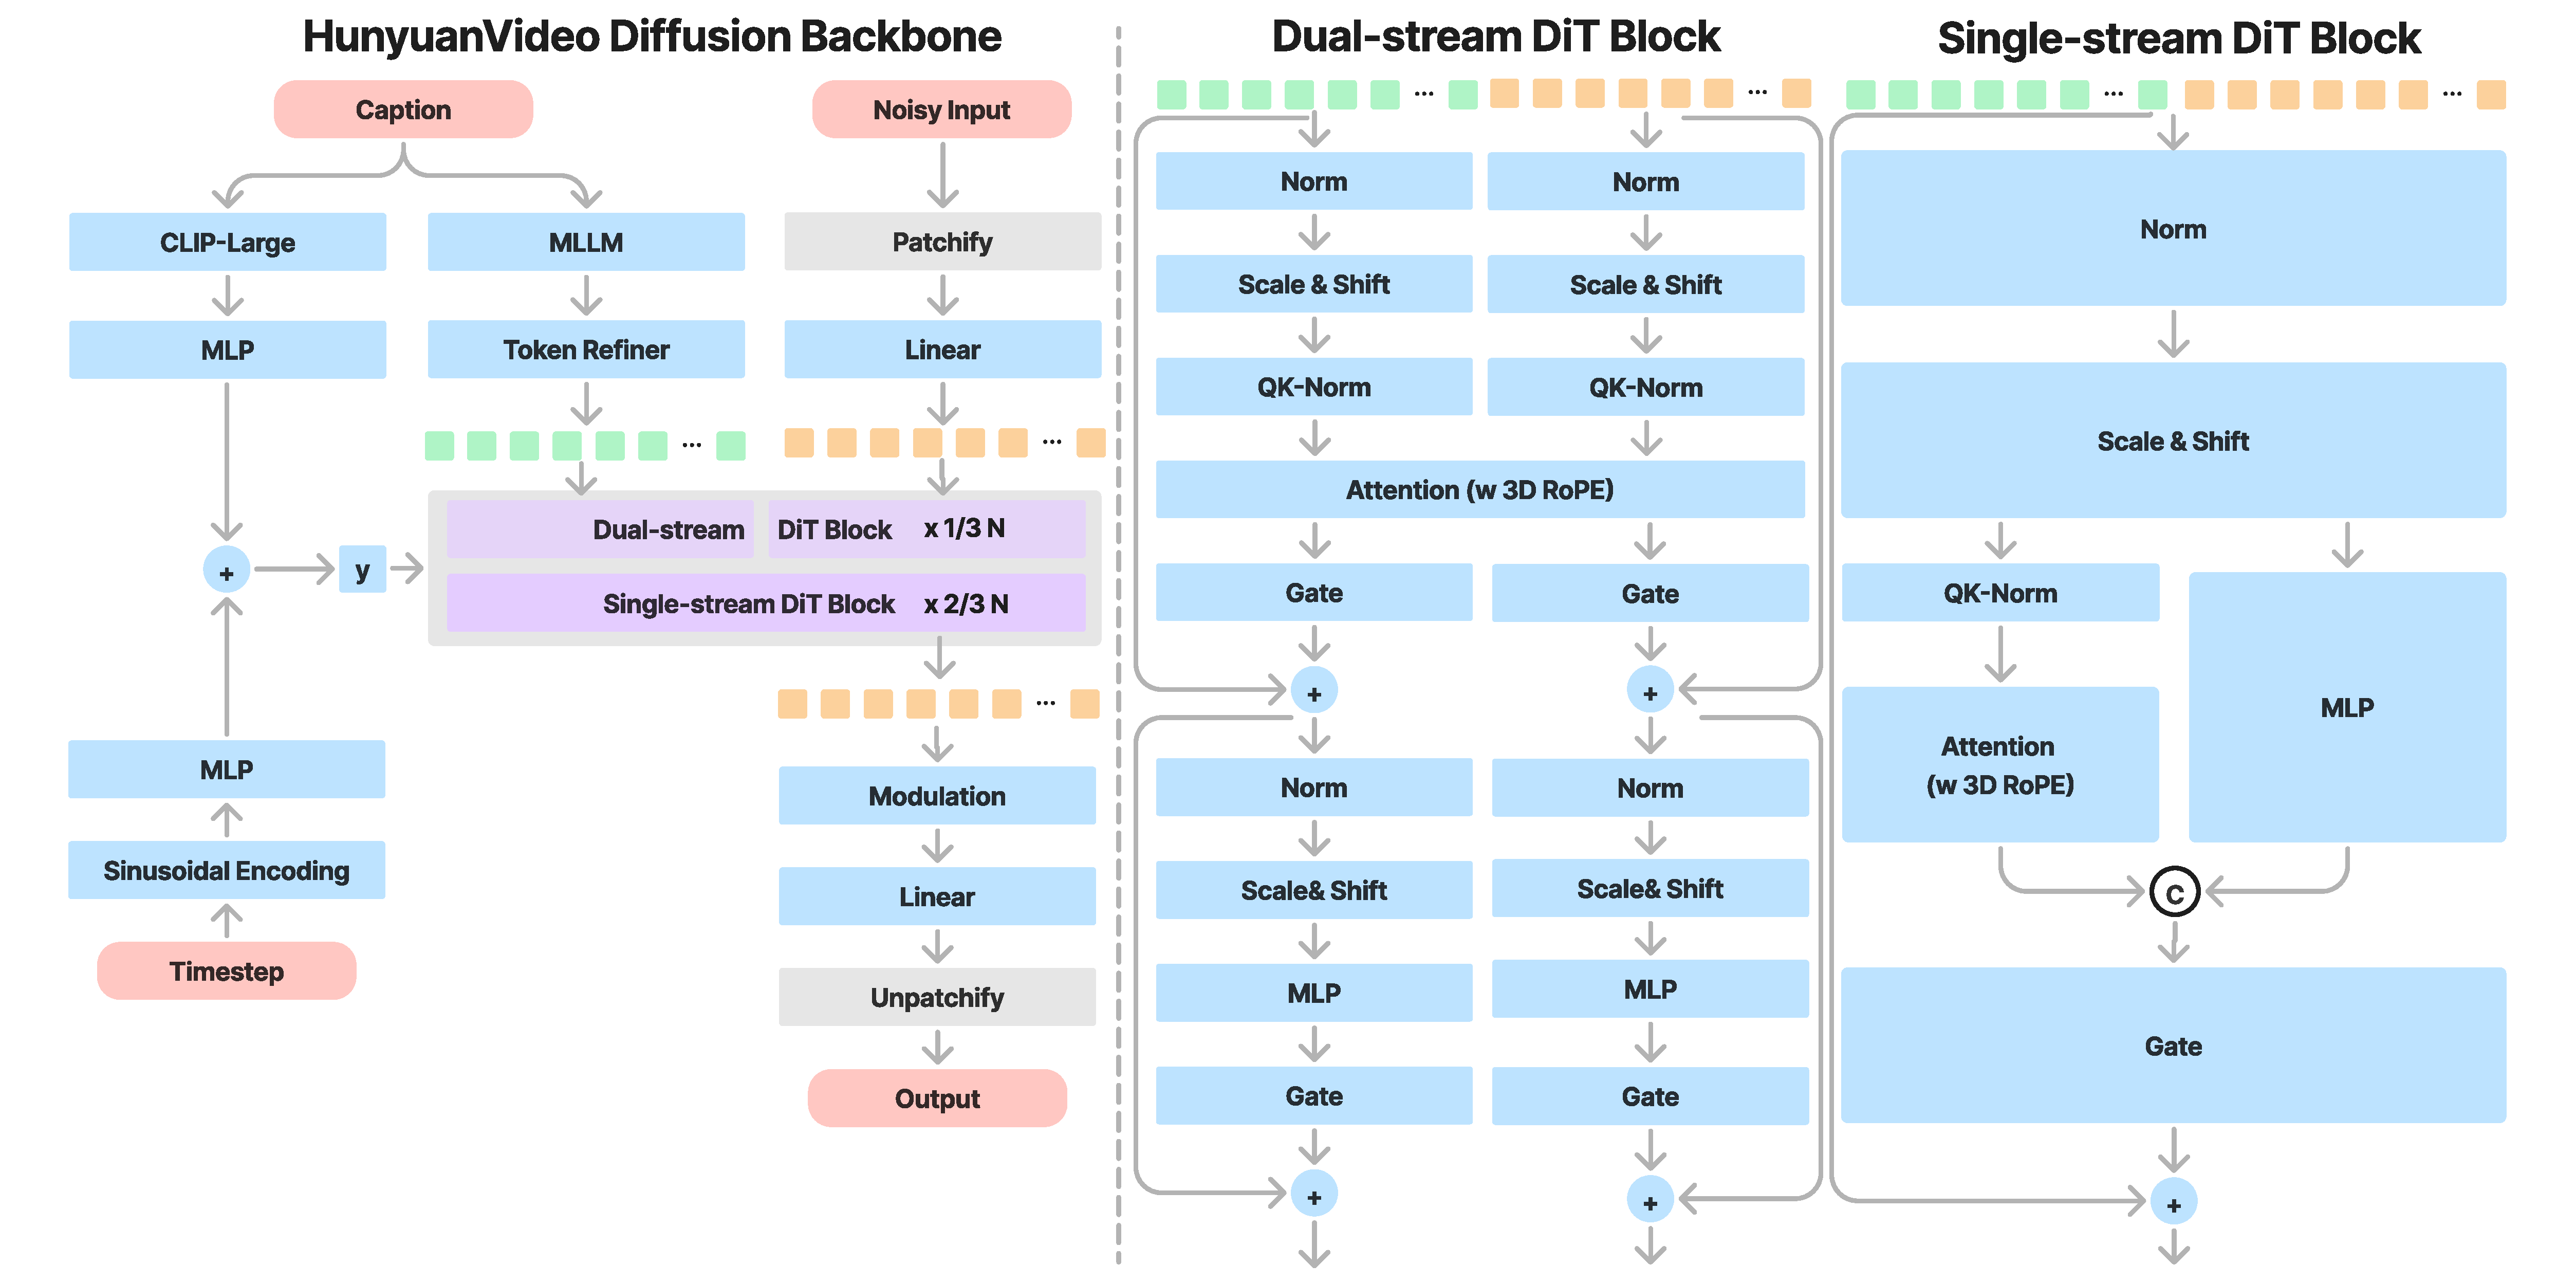
\includegraphics[width=\linewidth]{figures/dit_backbone.pdf}
    \caption{ The architecture of our \nameofmethod{} Diffusion Backbone.}
    \label{fig:dit_bnackbone}
\end{figure}

In this section, we introduce the Transformer design in \nameofmethod{}, which employs a unified Full Attention mechanism for three main reasons:
Firstly, it has demonstrated superior performance compared to divided spatiotemporal attention~\cite{videoworldsimulators2024,polyak2024movie,yang2024cogvideox,genmo2024mochi}.
Secondly, it supports unified generation for both images and videos, simplifying the training process and improving model scalability.
Lastly, it leverages existing LLM-related acceleration capabilities more effectively, enhancing both training and inference efficiency.
The model structure is illustrated in Figure \ref{fig:dit_bnackbone}.

\textbf{Inputs.} For a given video-text pair, the model operates within the 3D latent space described in Section \ref{3dVAE}. Specifically, for the video branch, the input is first compressed into latents of shape $T \times C \times H \times W$. To unify input processing, we treat images as single-frame videos. These latents are then patchified and unfolded into a 1D sequence of tokens with a length of $\frac{T}{k_t} \cdot \frac{H}{k_h} \cdot \frac{W}{k_w}$ using a 3D convolution with a kernel size of $k_t \times k_h \times k_w$. For the text branch, we first use an advanced LLM to encode the text into a sequence of embeddings that capture fine-grained semantic information. Concurrently, we employ the CLIP model to extract a pooled text representation containing global information. This representation is then expanded in dimensionality and added to the timestep embedding before being fed into the model.

\textbf{Model Design.}  To integrate textual and visual information effectively, we follow a similar strategy of "Dual-stream to Single-stream" hybrid model design as introduced in \cite{FLUX} for video generation. In the dual-stream phase, video and text tokens are processed independently through multiple Transformer blocks, enabling each modality to learn its own appropriate modulation mechanisms without interference. In the single-stream phase, we concatenate the video and text tokens and feed them into subsequent Transformer blocks for effective multimodal information fusion. This design captures complex interactions between visual and semantic information, enhancing overall model performance.

\textbf{Position Embedding.} To support multi-resolution, multi-aspect ratio, and varying duration generation, we use Rotary Position Embedding (RoPE)~\cite{su2023roformer} in each Transformer block. RoPE applies a rotary frequency matrix to the embeddings, enhancing the model's ability to capture both absolute and relative positional relationships, and demonstrating some extrapolation capability in LLMs. Given the added complexity of the temporal dimension in video data, we extend RoPE to three dimensions. Specifically, we compute the rotary frequency matrix separately for the coordinates of time ($T$), height ($H$), and width ($W$). We then partition the feature channels of the query and key into three segments $(d_t, d_h, d_w)$, multiply each segment by the corresponding coordinate frequencies and concatenate the segments. This process yields position-aware query and key embeddings, which are used for attention computation.

% This extension encodes spatial positions within each video frame and temporal positions across frames, improving the model's understanding and generation capabilities for video content.

For detailed model settings, please refer to Table~\ref{tab:model_settings}.
\begin{table}[t]
  \centering
  \footnotesize
  \caption{Architecture hyperparameters for the \nameofmethod{} 13B parameter foundation model.}
  \begin{tabular}{ccccccc}
  \toprule
  \textbf{\makecell{Dual-stream \\Blocks}} & \textbf{\makecell{Single-stream \\Blocks}} & \textbf{\makecell{Model \\Dimension}} & \textbf{\makecell{FFN \\Dimension}} & \textbf{\makecell{Attention \\Heads}} & \textbf{\makecell{Head dim}} & $(d_t, d_h, d_w)$	\\
  \midrule
  20 & 40 & 3072 & 12288 & 24 & 128 & (16, 56, 56) \\
  \bottomrule
  \end{tabular}%
  \label{tab:model_settings}
\end{table}

% This model architecture exhibits excellent performance and reduces computational complexity. Compared to fully single-stream models[][], visual and semantic tokens are processed separately in the dual-stream stage, resulting in fewer tokens and improved computational efficiency through parallel processing. Although more tokens need to be processed in the single-stream stage, the earlier stages have already extracted more refined features, thereby reducing the overall training complexity.

\subsection{Text encoder}
% \dq{@Zijian, Jianwei, Weijie, Tianqi}

In generation tasks like text-to-image and text-to-video, the text encoder plays a crucial role by providing guidance information in the latent space. Some representative works~\cite{podell2023sdxl, esser2024scaling, li2024hunyuandit} typically use pre-trained CLIP~\cite{radford2021learning} and T5-XXL~\cite{raffel2020exploring} as text encoders where CLIP uses Transformer Encoder and T5 uses an Encoder-Decoder structure. In contrast, we utilize a pre-trained Multimodal Large Language Model~(MLLM) with a Decoder-Only structure as our text encoder, which has following advantages: (i) Compared with T5, MLLM after visual instruction finetuning has better image-text alignment in the feature space, which alleviates the difficulty of instruction following in diffusion models; (ii) Compared with CLIP, MLLM has been demonstrated superior ability in image detail description and complex reasoning~\cite{liu2024visual}; (iii) MLLM can play as a zero-shot learner~\cite{brown2020language} by following system instructions prepended to user prompts, helping text features pay more attention to key information. In addition, as shown in Fig.~\ref{fig:text-encoder}, MLLM is based on causal attention while T5-XXL utilizes bidirectional attention that produces better text guidance for diffusion models. Therefore, we follow~\cite{ma2024exploring} to introduce an extra bidirectional token refiner for enhancing text features.
%
We have configured \nameofmethod{} with a series of MLLMs~\cite{sun2024hunyuanlargeopensourcemoemodel,2023xtuner,glm2024chatglm} for different purposes. Under each setting, MLLMs have shown superior performance over conventional text encoder.
% With extensive experiments, we have demonstrated the effectiveness of MLLM as the text encoder on smaller \nameofmethod{} by integrating various open-source MLLMs~\cite{sun2024hunyuanlargeopensourcemoemodel,2023xtuner,glm2024chatglm}.

In addition, CLIP text features are also valuable as the summary of the text information. As shown in Fig.~\ref{fig:dit_bnackbone} We adopt the final non-padded token of CLIP-Large text features as a global guidance, integrating into the dual-stream and single-stream DiT blocks. 

\begin{figure}[t]
    \centering
    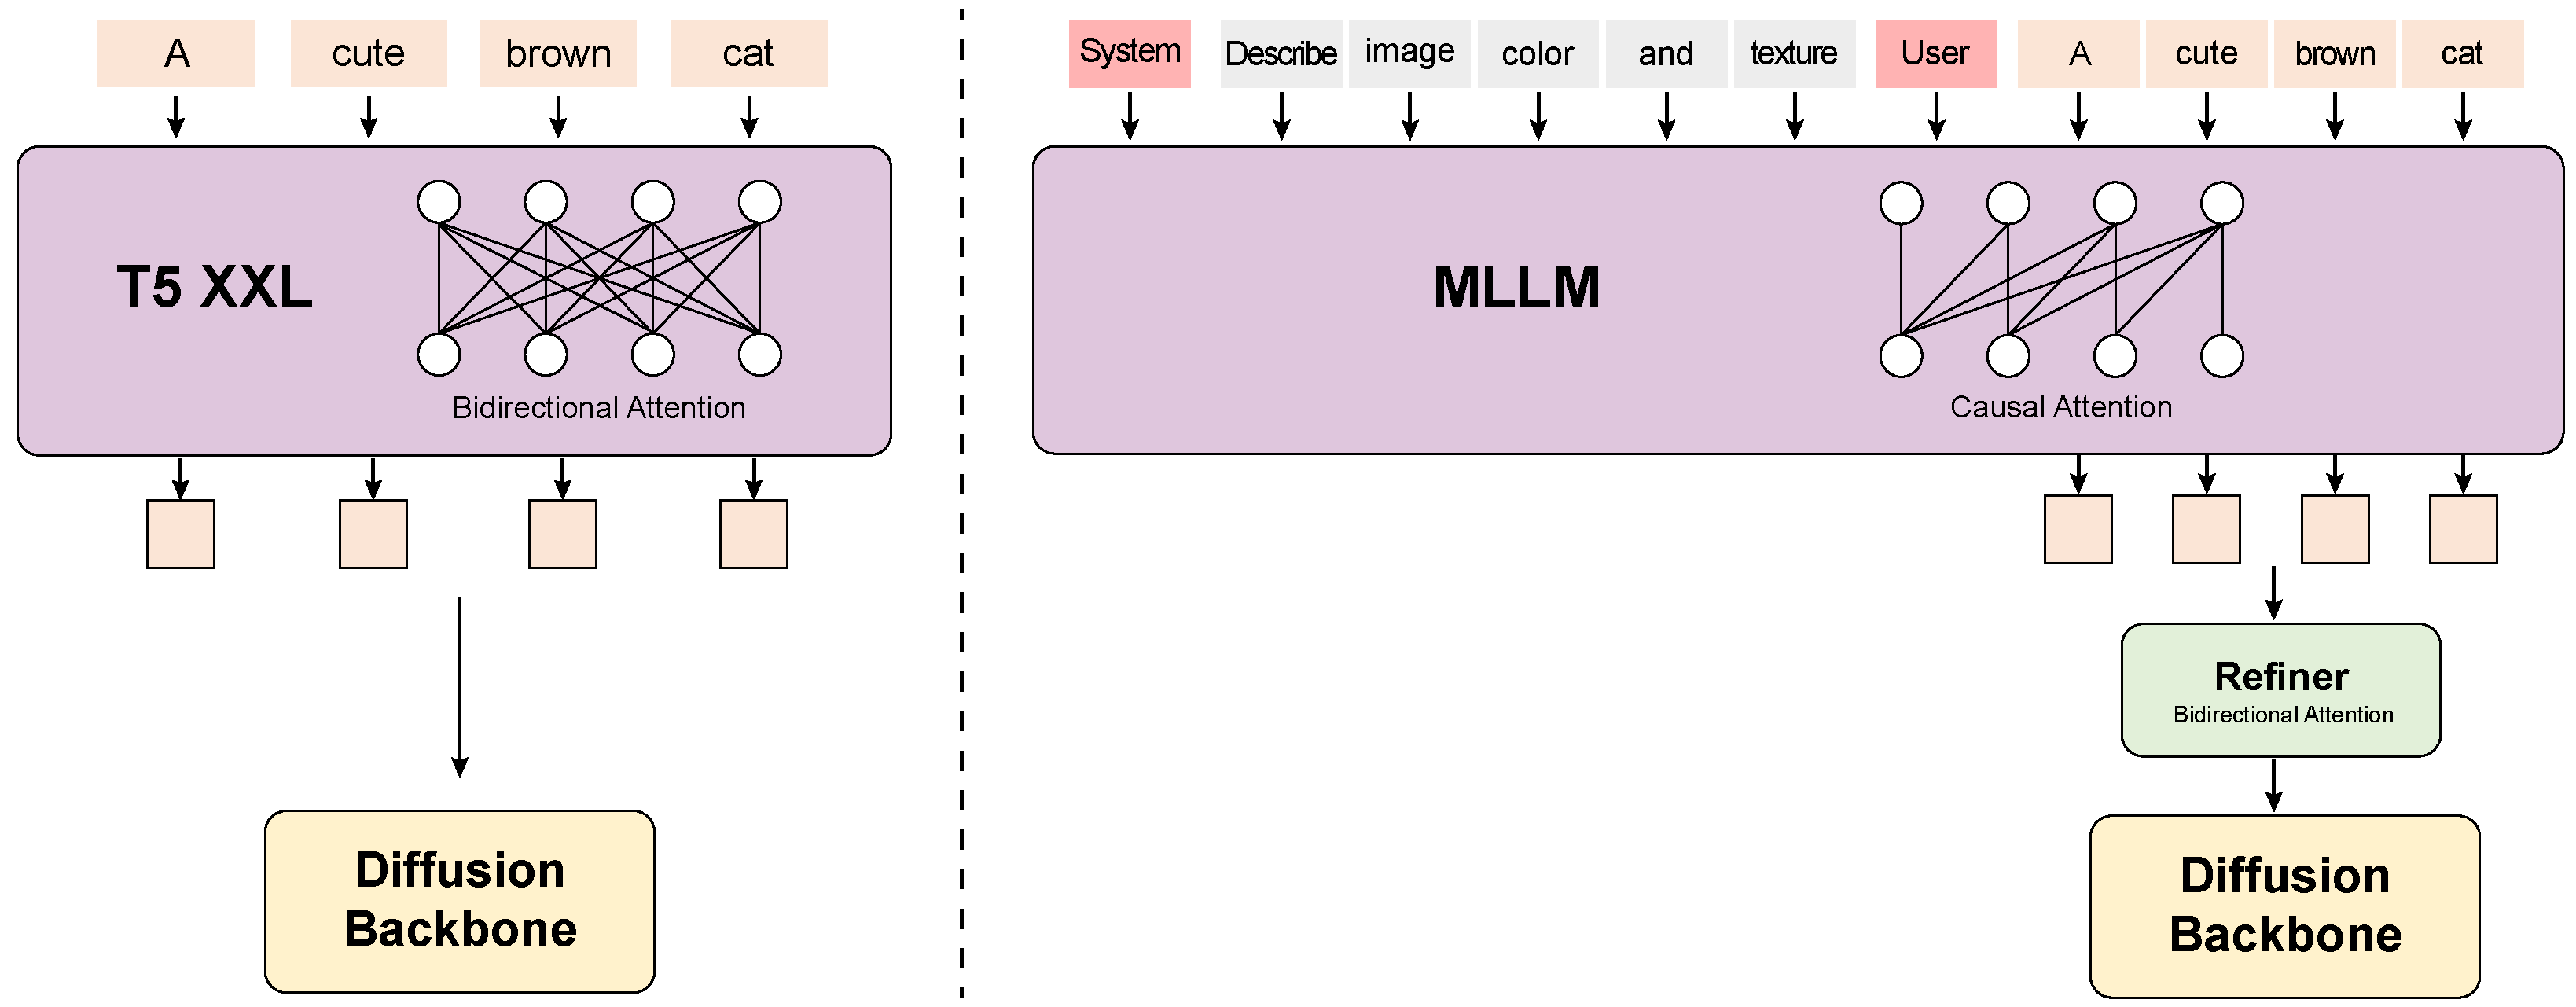
\includegraphics[width=0.9\linewidth]{figures/text_encoder_en.pdf}
    \caption{Text encoder comparison between T5 XXL and the instruction-guided MLLM introduced by \nameofmethod{}.}
    \label{fig:text-encoder}
\end{figure}


\subsection{Model Scaling}
Neural scaling laws~\cite{kaplan2020scaling,hoffmann2022training} in language model training offer a powerful tool for understanding and optimizing the performance of machine learning models. By elucidating the relationships between model size ($N$), dataset size ($D$), and computational resources ($C$), these laws help drive the development of more effective and efficient models, ultimately advancing the success of large model training.

\begin{figure}[t]
    \centering
    \begin{subfigure}{0.325\textwidth}
        \centering
        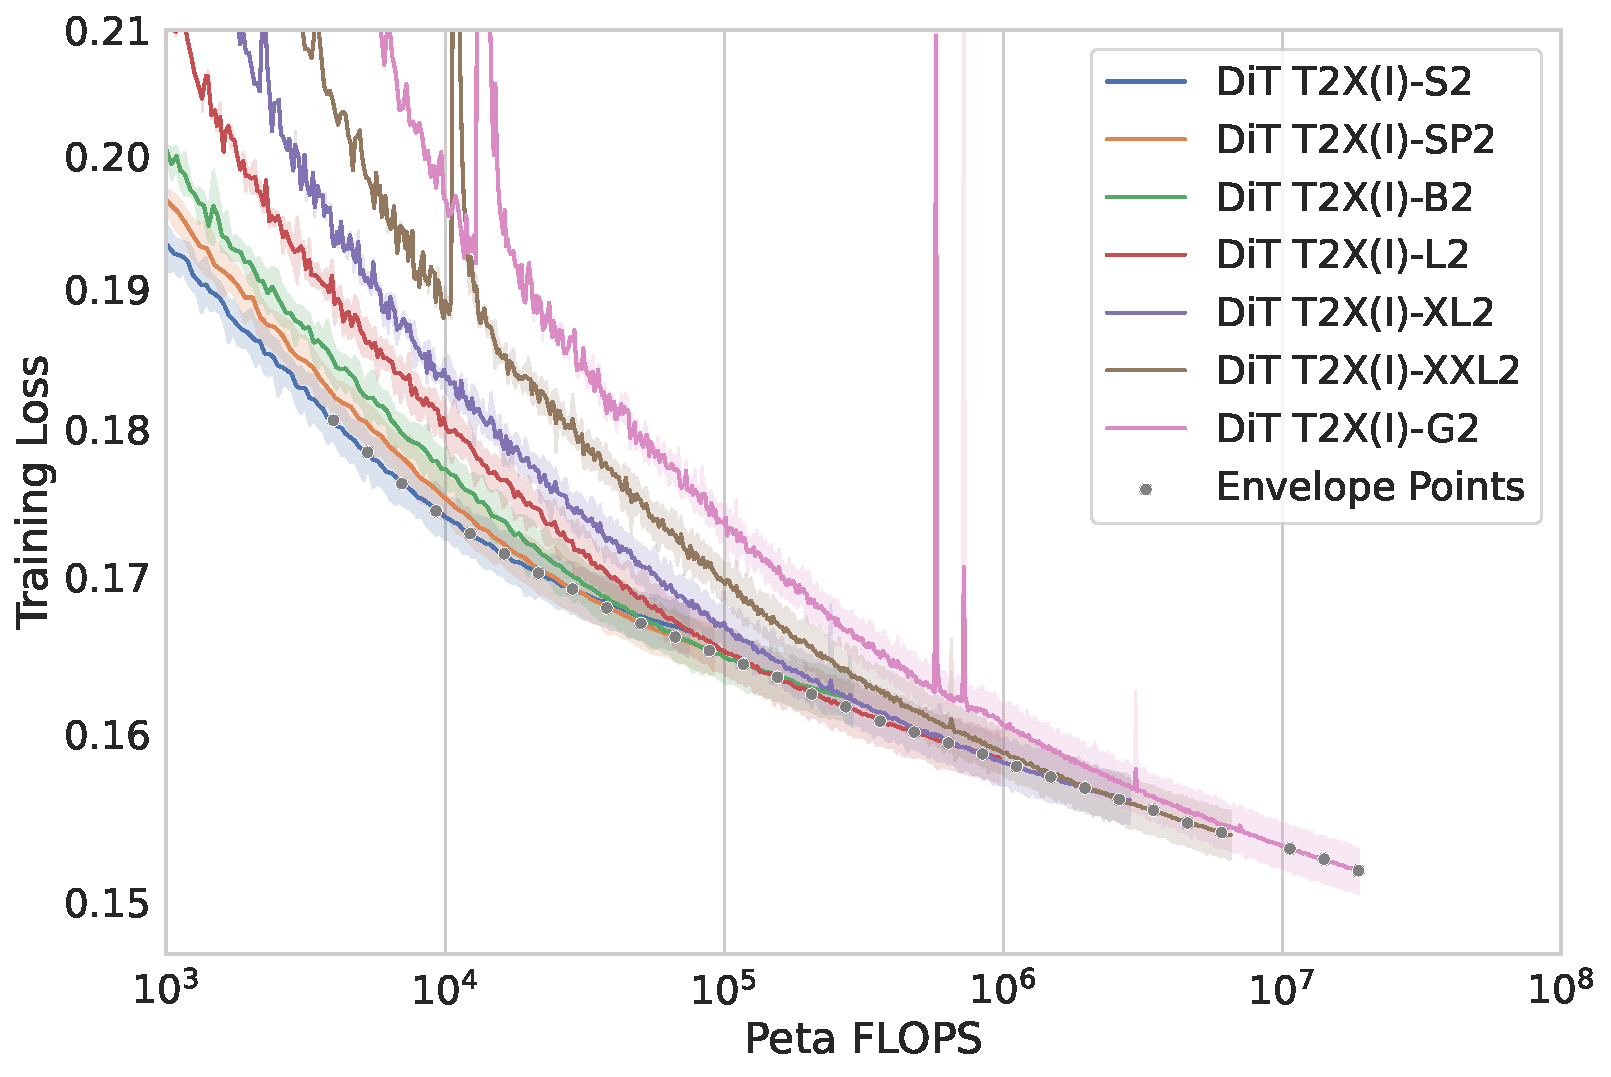
\includegraphics[width=\textwidth]{figures/scaling_law.pdf}
        \caption{T2X(I) Loss curve and envelope}
        \label{fig:scaling-laws}
    \end{subfigure}
    \hfill
    \begin{subfigure}{0.325\textwidth}
        \centering
        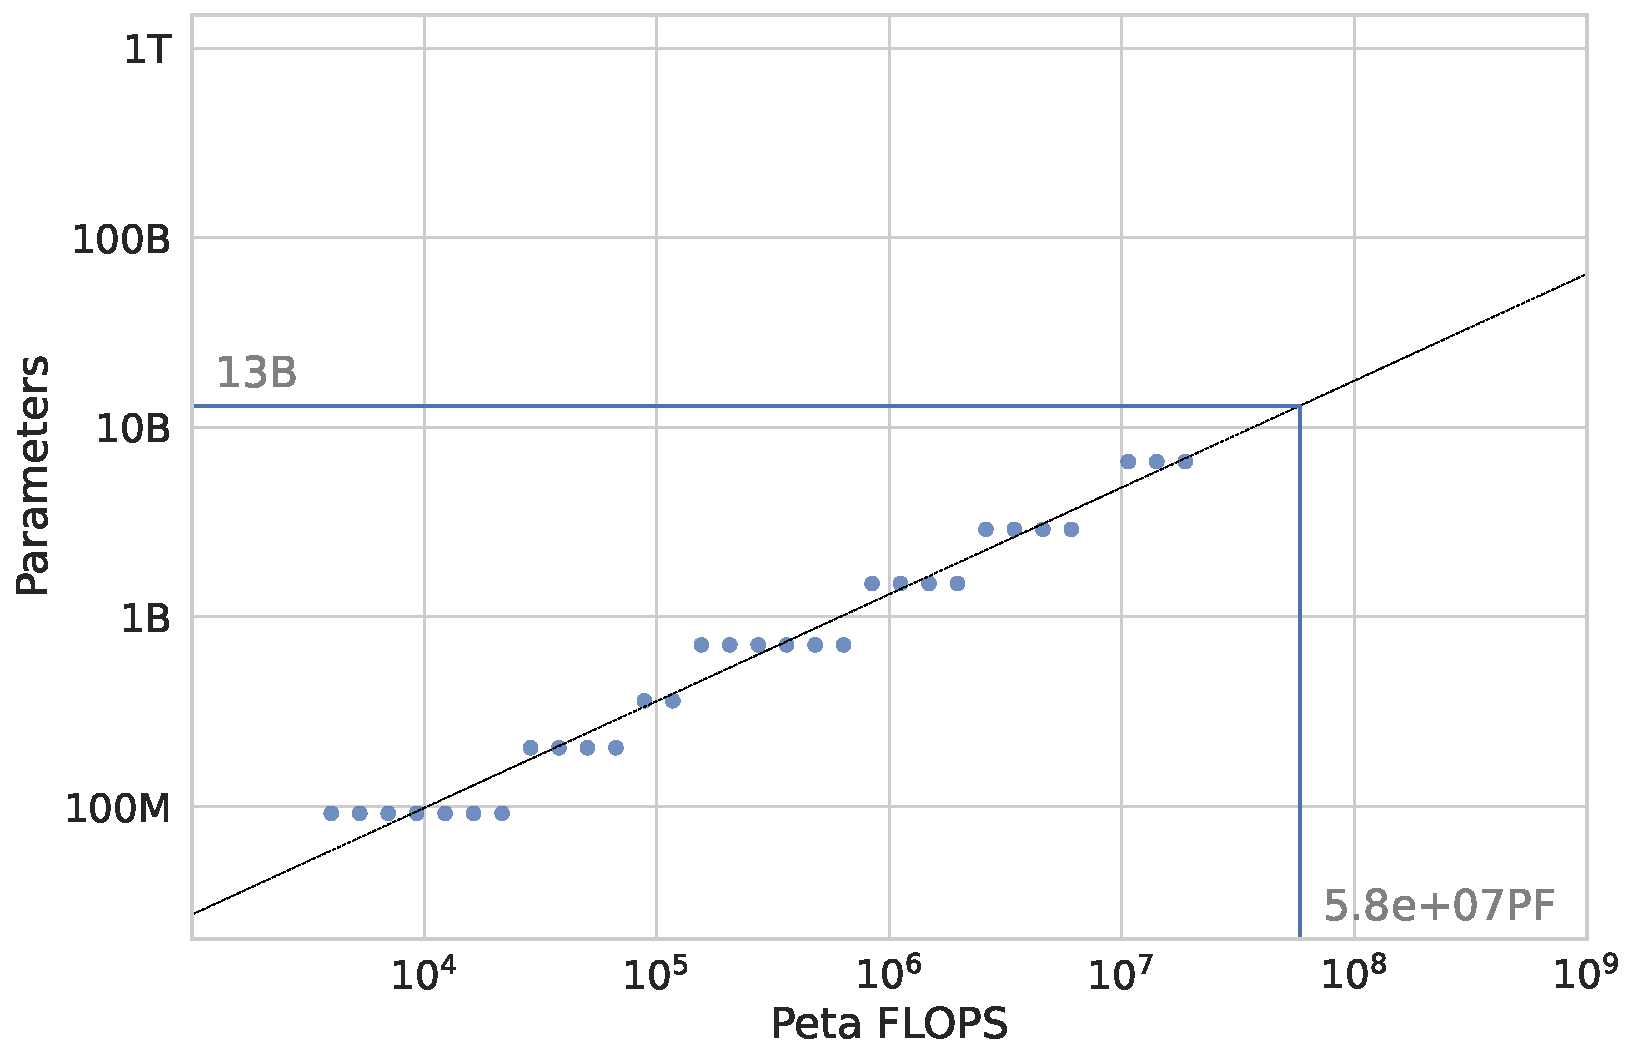
\includegraphics[width=\textwidth]{figures/computation_vs_parameter.pdf}
        \caption{T2X(I) Power law of $C$ and $N$}
        \label{fig:computation-vs-parameter}
    \end{subfigure}
    \hfill
    \begin{subfigure}{0.325\textwidth}
        \centering
        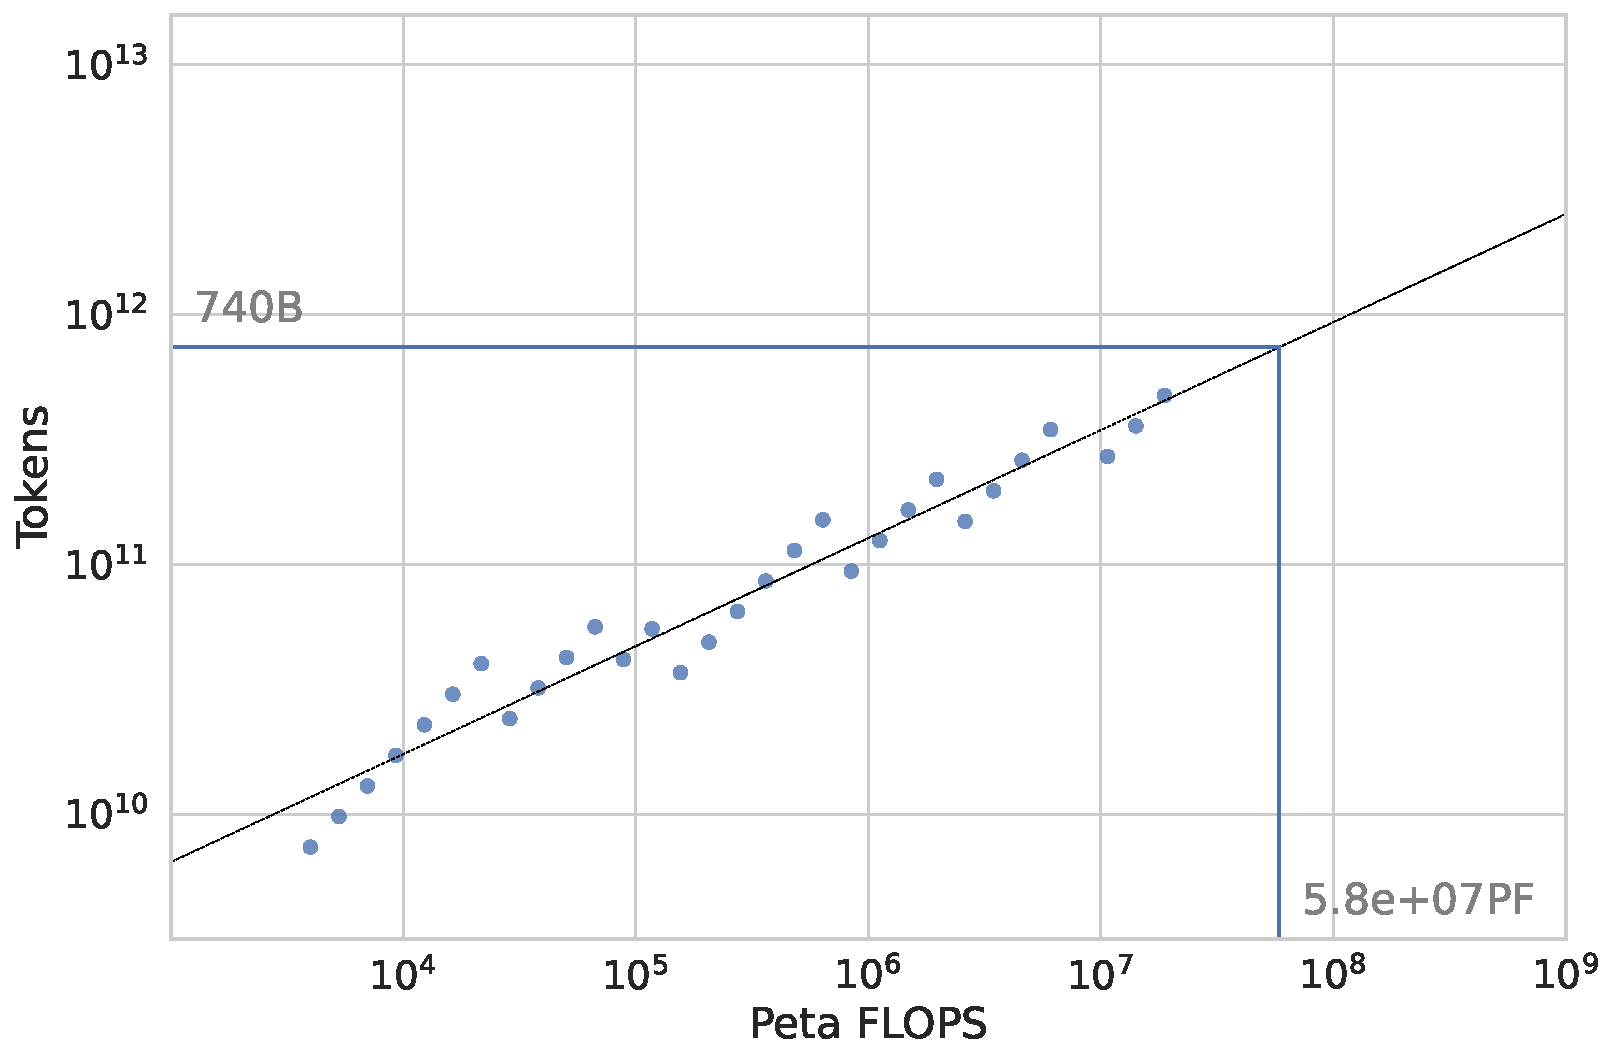
\includegraphics[width=\textwidth]{figures/computation_vs_token.pdf}
        \caption{T2X(I) Power law of $C$ and $D$}
        \label{fig:computation-vs-token}
    \end{subfigure}
    \hfill
    \begin{subfigure}{0.325\textwidth}
        \centering
        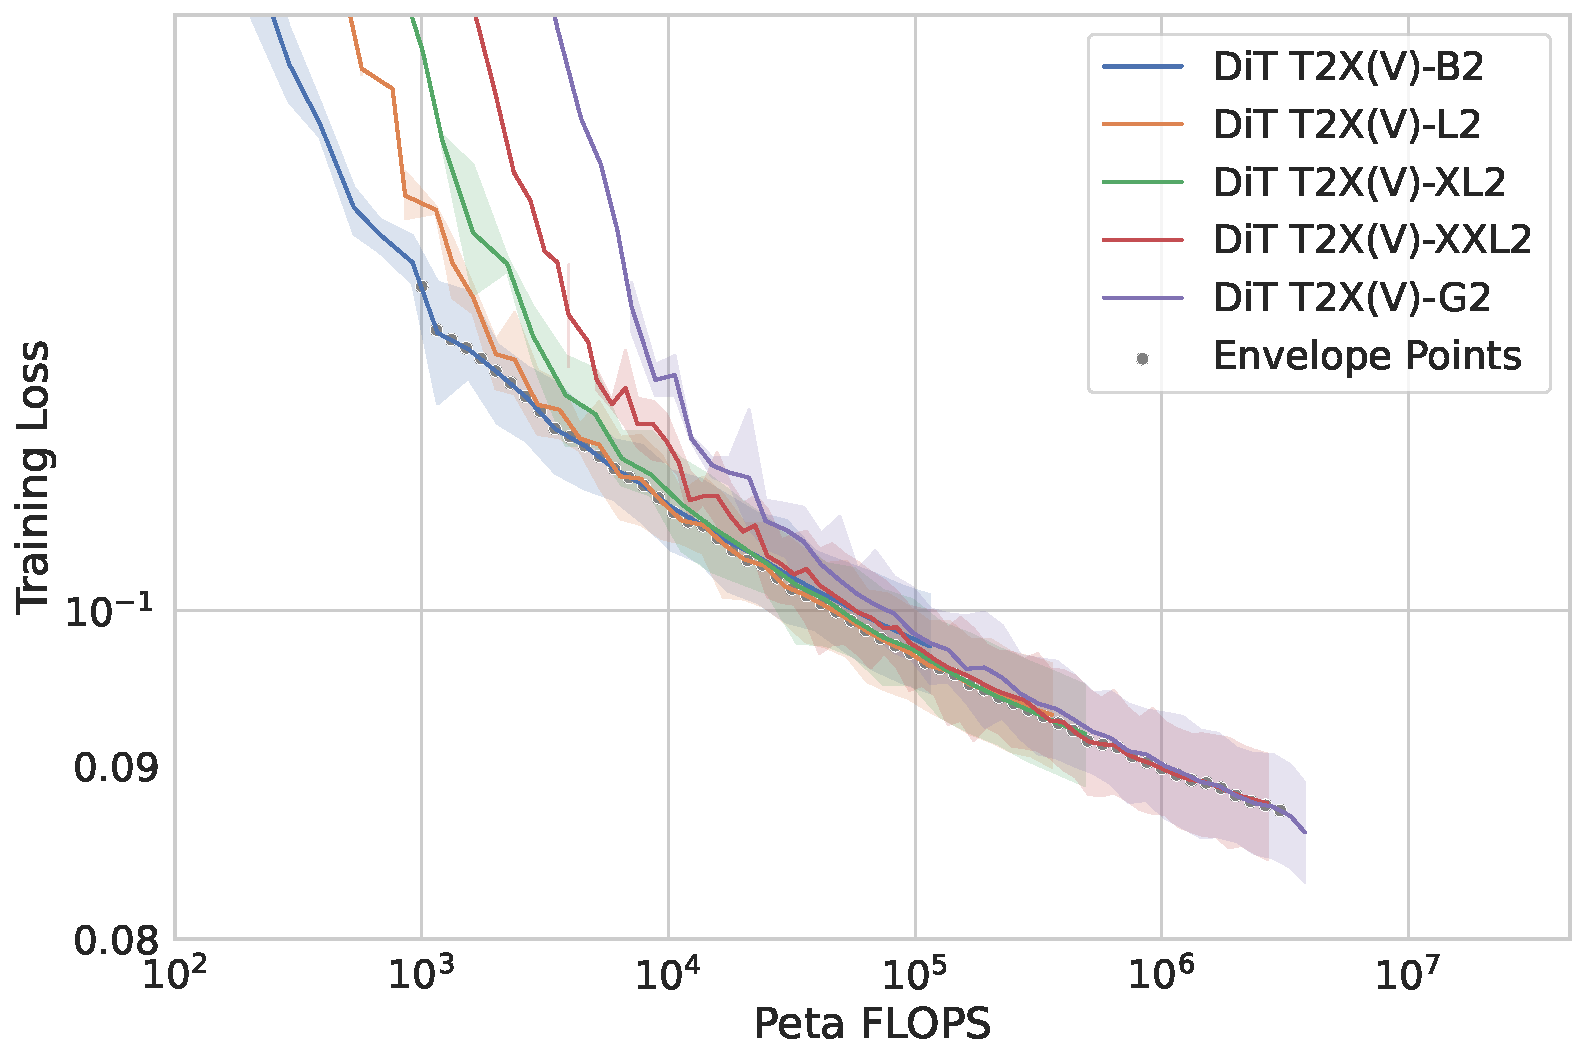
\includegraphics[width=\textwidth]{figures/video_scaling_law.pdf}
        \caption{T2X(V) Loss curve and envelope}
        \label{fig:video-scaling-laws}
    \end{subfigure}
    \hfill
    \begin{subfigure}{0.325\textwidth}
        \centering
        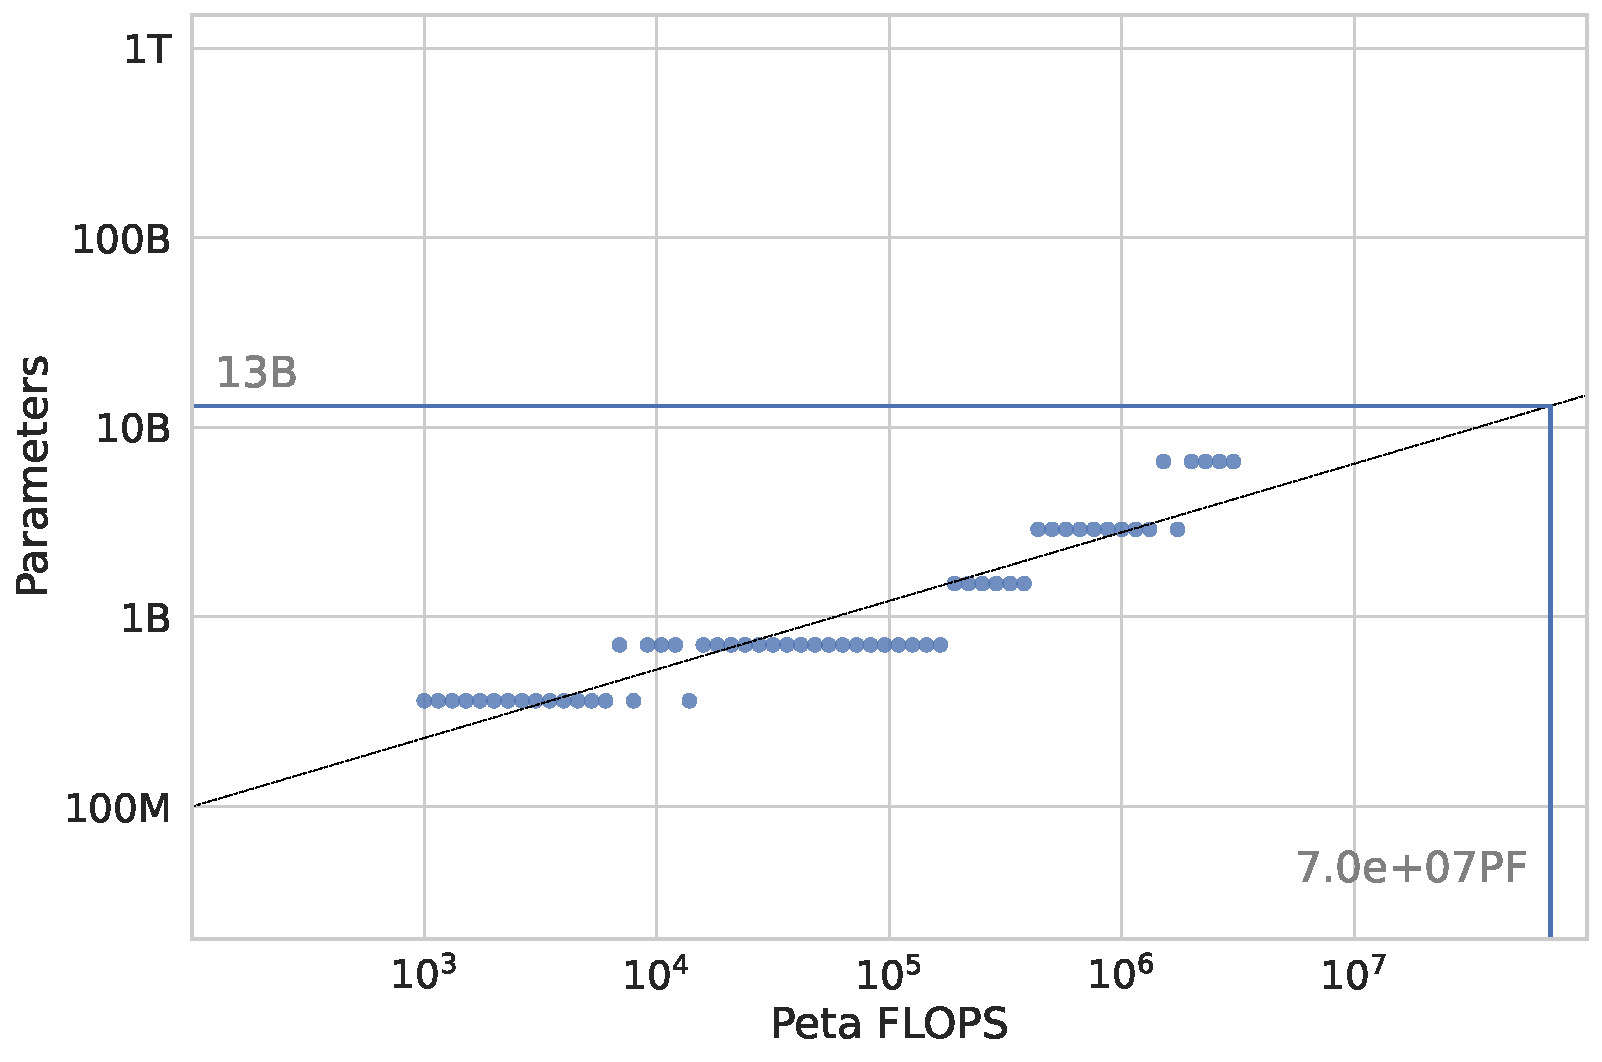
\includegraphics[width=\textwidth]{figures/video_computation_vs_parameter.pdf}
        \caption{T2X(V) Power law of $C$ and $N$}
        \label{fig:video-computation-vs-parameter}
    \end{subfigure}
    \hfill
    \begin{subfigure}{0.325\textwidth}
        \centering
        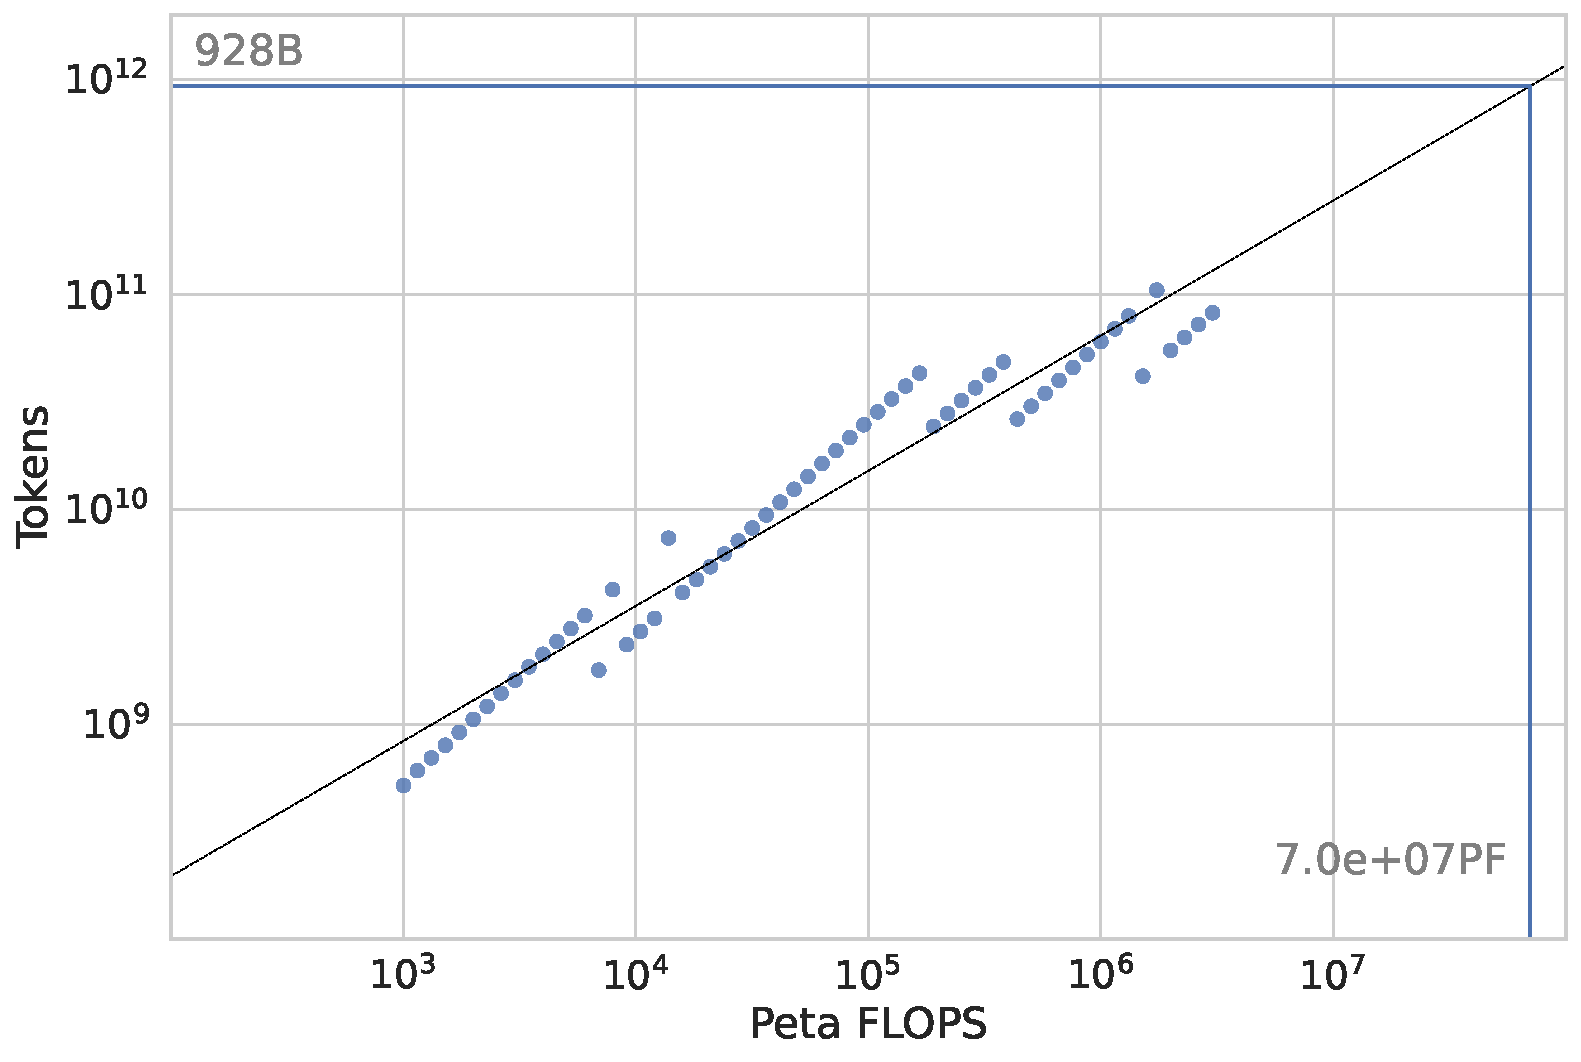
\includegraphics[width=\textwidth]{figures/video_computation_vs_token.pdf}
        \caption{T2X(V) Power law of $C$ and $D$}
        \label{fig:video-computation-vs-token}
    \end{subfigure}
    \caption{Scaling laws of DiT-T2X model family. On the top-left (a) we show the loss curves of the T2X(I) model on a log-log scale for a range of model sizes from 92M to 6.6B. We follow~\cite{hoffmann2022training} to plot the envelope in gray points, which are used to estimate the power-law coefficients of the amount of computation ($C$) vs model parameters ($N$) (b) and the computation vs tokens ($D$) (c). Based on the scaling law of the T2X(I) model, we plot the scaling law of the corresponding T2X(V) model in (d), (e), and (f).}
    \label{fig:image_scaling_laws}
\end{figure}

In contrast to prior scaling laws on large language models~\cite{kaplan2020scaling,hoffmann2022training,touvron2023llama,achiam2023gpt,anil2023palm} and image generation models~\cite{li2024scalability,kilian2024computational}, video generation models typically rely on pre-trained image models. Consequently, our initial step involved establishing the foundational scaling laws pertinent to text-to-image. Building upon these foundational scaling laws, we subsequently derived the scaling laws applicable to the text-to-video model. By integrating these two sets of scaling laws, we were able to systematically determine the appropriate model and data configuration for video generation tasks. 

% Specifically, we developed a series of models with sizes ranging from 92M to 6.6B. Each model was trained on up to 500 billion tokens, using consistent hyperparameters and the same dataset with 256p resolution. By examining the final loss of these models, we refer to \cite{hoffmann2022training} to establish the relationship between training FLOPs $C$ and model parameters $N$ as $ N = a\cdot C^{b}$, where $a$ and $b$ denotes the coefficient to be fitted.

\subsubsection{Image model scaling law}
% \dq{@Zijian, Jianwei}

Kaplan et.al~\cite{kaplan2020scaling} and Hoffmann et.al~\cite{hoffmann2022training} explored emperical scaling laws for language models on cross-entropy loss. In the field of diffusion based visual generation, Li et.al~\cite{li2024scalability} study the scaling properties on UNet, while transformer based works such as DiT~\cite{peebles2023scalable}, U-ViT~\cite{bao2023all}, Lumina-T2X~\cite{gao2024lumina}, and SD3~\cite{esser2024scaling} only study the scaling behavior between sample quality and network complexity, leaving the power-laws about the computation resources and MSE loss used by diffusion models unexplored.

In order to fill the gap, we develop a family of DiT-like models, named as DiT-T2X to distinguish from the original DiT, where X can be the image (I) or the video (V).
DiT-T2X applies T5-XXL~\cite{raffel2020exploring} as the text encoder and the aformentioned 3D VAE as the image encoder. The text information is injected to the model according to cross-attention layers. The DiT-T2X family has seven sizes ranging from 92M to 6.6B. The models were trained using DDPM~\cite{ho2020denoising} and v-prediction~\cite{salimans2022progressive} with consistent hyperparameters and the same dataset with 256px resolution. We follow the experiment method introduced by~\cite{hoffmann2022training} and build the neural scaling laws to fit 
\begin{equation}\label{eq:scaling_law}
N_{opt}=a_1C^{b_1},\quad D_{opt}=a_2C^{b_2}.    
\end{equation}

As shown in Fig.~\ref{fig:image_scaling_laws} (a), the loss curve of each model decreases from top left to bottom right, and it always passes through the loss curve of the larger size model adjacent to it. It means that each curve will form two intersections with curves of the larger and the smaller models. Under the corresponding computation resources between the two intersections, the middle-sized model is optimal (with the lowest loss). After obtaining the envelope of lowest losses across all the x-axis values, we fill the Equation ~\eqref{eq:scaling_law} to find out that $a_1=5.48\times10^{-4}, b_1=0.5634, a_2=0.324$ and $b_2=0.4325$, where the units of $a_1, a_2, N_{opt}, D_{opt}$ are billions while $C$ has a unit of Peta FLOPs. The Fig.~\ref{fig:image_scaling_laws} (b) and Fig.~\ref{fig:image_scaling_laws} (c) show that DiT-T2X(I) family fits the power law quite well. Finally, given computation budgets, we can calculate the optimal model size and dataset size. 

\subsubsection{Video model scaling law}
Based on the scaling law of the T2X(I) model, we select the optimal image checkpoint (\textit{i.e.,} the model on the envelope) corresponding to each size model to serve as the initialization model for the video scaling law experiment. Fig.~\ref{fig:image_scaling_laws} (d), Fig.~\ref{fig:image_scaling_laws} (e), and Fig.~\ref{fig:image_scaling_laws} (f) illustrate the scaling law results of the T2X(V) model, where $a_1=0.0189, b_1=0.3618, a_2=0.0108$ and $b_2=0.6289$.
Based on the results of Fig.~\ref{fig:image_scaling_laws} (b) and Fig.~\ref{fig:image_scaling_laws} (e), and taking into account the training consumption and inference cost, we finally set the model size to 13B. Then the number of tokens for image and video training can be calculated as shown in Fig.~\ref{fig:image_scaling_laws} (c) and Fig.~\ref{fig:image_scaling_laws} (f). It is worth noting that the amount of training tokens calculated by image and video scaling laws is only related to the first stage of training for images and videos respectively. The scaling property of progressive training from low-resolution to high-resolution will be left explored in future work.

% \dq{@Tianqi, Weijie}





\subsection{Model-pretraining}\label{model-pretrain}
% \subsubsection{Overview}
We use Flow Matching~\cite{lipman2022flow} for model training and split the training process into multiple stages. We first pretrain our model on 256px and 512px images, then conduct joint training on images and videos from 256px to 960px. 
% Our training is composed of multiple stages. We first pretrain our model on 256px $\rightarrow$ 512px images, then conduct joint training on images and videos from 256px to 720px. 


\subsubsection{Training Objective}
% \kathy{better move this  }
In this work, we employ the Flow Matching framework~\cite{lipman2022flow,esser2024scaling,chen2018neural} to train our image and video generation model. Flow Matching transforms a complex probability distribution into a simple probability distribution through a series of variable transformations of the probability density function, and generates new data samples through inverse transformations.

During the training process, given an image or video latent representation ${\rm \bf{x}}_1$ in the training set. We first sample $t\in [0,1]$  from a logit-normal distribution~\cite{esser2024scaling} and initialize a noise ${\rm \bf{x}}_0 \sim \mathcal{N}({\rm \bf{0}}, {\rm \bf{I}})$ following Gaussion distribution. The training sample ${\rm \bf{x}}_t$ is then constructed using a linear interpolation method~\cite{lipman2022flow}. The model is trained to predict the velocity ${\rm \bf{u}}_t=d {\rm \bf{x}}_t/dt$, which guides the sample ${\rm \bf{x}}_t$ towards the sample ${\rm \bf{x}}_1$. The model parameters are optimized by minimizing the mean squared error between the predicted velocity ${\rm \bf{v}}_t$ and the ground truth velocity ${\rm \bf{u}}_t$, expressed as the loss function
\begin{equation}
  \label{eq:fm}
  \mathcal{L}_{{\rm generation}}=\mathbb{E}_{t,{\rm \bf{x}}_0,{\rm \bf{x}}_1}\|{\rm \bf{v}}_t - {\rm \bf{u}}_t  \|^2.
\end{equation}

During the inference process, a noise sample ${\rm \bf{x}}_0 \sim \mathcal{N}({\rm \bf{0}}, {\rm \bf{I}})$ is drawn initially. The first-order Euler ordinary differential equation (ODE) solver is then used to compute ${\rm \bf{x}}_1$ by integrating the model's estimated values for $d{\rm \bf{x}}_t/dt$. This process ultimately generates the final sample ${\rm \bf{x}}_1$.
% which reflects the characteristics of the target distribution. 
% These processes enable the model to learn the transformation from a simple distribution to a complex one during training and to generate new samples from the learned distribution during inference.

\subsubsection{Image Pre-training}
% \myPara{Image Pre-training}
% \dq{@Jian Wei, Zijian, Wuyue, Yanxin}
% We have validated the optimal network structure through detailed experiments including modulation module design, architecture of DiT block, different denosier scheme and text encoders. The overview of our network is shown in Fig.[]. 

At our early experiments, we found that a well pretrained model significantly accelerates the convergence of video training and improves video generation performance. Therefore, we introduce a two-stage progressive image pretraining strategy to serve as a warmup for video training. 

\textbf{Image stage 1 (256px training).} The model is first pretrained with low-resolution 256px images. Specifically, we follow previous work~\cite{podell2023sdxl} to enable multi-aspect training based on 256px, which helps the model learn to generate images with a wide range of aspect ratios while avoiding the text-image misalignments caused by the crop operation in image preprocessing. Meanwhile, pretraining with low resolution samples allows the model to learn more low-frequency concepts from a larger amount of samples. 

\textbf{Image stage 2 (mix-scale training).} We introduce a second image-pretraining stage to further facilitate the model ability on higher resolutions, such as 512px. A trivial solution is to directly funetuning on images based on 512px. However, we found that the model performance finetuned on 512px images will degrade severely on 256px image generation, which may affect the following video pretraining on 256px videos. Therefore, we propose \textit{mix-scale training}, where two or more scales of multi-aspect buckets are included for each training global batch. Each scale have an anchor size, and then the multi-aspect buckets are built based on the anchor size. We train the model on a two-scale dataset with anchor sizes 256px and 512px for learning higher resolution images while maintaining the ability on low resolutions. We also introduce dynamic batch sizes for micro batches with different image scales, maximaizing the GPU memory and computation utilization.


\subsubsection{Video-Image joint training}
% \myPara{Video-Image Joint-training}
% \dq{@Weijie, Tianqi, Daquan}

\textbf{Multiple aspect ratios and durations bucketization.}  After the data filtering process described in Section \ref{data_filtering}, the videos have different aspect ratios and durations. To effectively utilize the data, we categorize the training data into buckets based on duration and aspect ratio. We create $B_T$ duration buckets and $B_{AR}$ aspect ratio buckets, resulting in a total of $B_T \times B_{AR}$ buckets. As the number of tokens varies across buckets, we assign each bucket a maximum batch size that can prevent out-of-memory (OOM) errors, to optimize GPU resource utilization. Before training, all data is allocated to the nearest bucket. During training, each rank randomly pre-fetches batch data from a bucket. This random selection ensures the model is trained on varying data sizes at each step, which helps maintain model generalization by avoiding the limitations of training on a single size.

\textbf{Progressive Video-Image Joint Training.} Generating high-quality, long-duration video sequences directly from text often leads to difficulties in model convergence and suboptimal results. Therefore, progressive curriculum learning has become a widely adopted strategy for training text-to-video models. In \nameofmethod{}, we designed a comprehensive curriculum learning strategy, starting with model initialization using T2I parameters and progressively increasing video duration and resolution.

\begin{itemize}
\item \textbf{Low-resolution, short video stage.} The model establishes the basic mapping between text and visual content, ensuring consistency and coherence in short-term actions.

\item \textbf{Low-resolution, long video stage.} The model learns more complex temporal dynamics and scene changes, ensuring temporal and spatial consistency over a longer duration.

\item \textbf{High-resolution, long video stage.} The model enhances video resolution and detail quality while maintaining temporal coherence and managing complex temporal dynamics.
\end{itemize}

Additionally, at each stage, we incorporate images in varying proportions for video-image joint training. This approach addresses the scarcity of high-quality video data, enabling the model to learn more extensive and diverse world knowledge. It also effectively prevents catastrophic forgetting of image-space semantics due to distributional discrepancies between video and image data.

\subsection{Prompt Rewrite} 
To address the variability in linguistic style and length of user-provided prompts, we employ the Hunyuan-Large model \cite{sun2024hunyuanlargeopensourcemoemodel} as our prompt rewrite model to adapt the original user prompt to the model-preferred prompt. Utilized within a training-free framework, the prompt rewrite model capitalizes on detailed prompt instructions and in-context learning examples to enhance its performance. The key functionalities of this prompt rewrite module are as follows:

\begin{itemize}
    \item \textbf{Multilingual Input Adaptation}: The module is designed to process and comprehend user prompts across various languages, ensuring that meaning and context are preserved.
    \item \textbf{Standardization of Prompt Structure}: The module rephrases prompts to conform to a standardized information architecture, akin to training captions.
    \item \textbf{Simplification of Complex Terminology}: The module simplifies complex user wording into more straightforward expressions, all while maintaining the user's original intent.
\end{itemize}

Furthermore, we implement a self-revision technique \cite{kim2024reex} to refine the final prompt. This involves a comparative analysis between the original prompt and the rewritten version, ensuring that the output is both accurate and aligned with the model's capabilities.

To accelerate and simplify the application process, we also fine-tune a Hunyuan-Large model with LoRA for prompt rewriting. The training data for this LoRA tuning was sourced from the high-quality rewrite pairs collected through the training-free method.


\subsection{High-performance Model Fine-tuning}\label{sft}
In the pre-training stage, we utilized a large dataset for model training. While this dataset is rich in information, it displayed considerable variability in data quality. To create a robust generation model capable of producing high-quality, dynamic videos and improving its proficiency in continuous motion control and character animation, we carefully selected four specific subsets from the full dataset for fine-tuning.
These subsets underwent an initial screening using automated data filtering techniques, followed by manual review. Additionally, we implemented various model optimization strategies to maximize generation performance.

% The fine-tuning strategy adheres to a sequential process of independent training followed by model merging. Specifically, we first identified the optimal checkpoint in the pre-training stage, and then this checkpoint serves as the initialization parameter for subsequent fine-tuning of the model across the four designated subsets.
% Finally, we employ model merging based on the optimal pre-training model and the four fine-tuned models, and determine the final fusion model by performing a grid search on the fusion coefficient.

% \dq{@Tianqi, Weijie, Daquan}

% \input{tax/t2v}

\section{Model Acceleration}
\label{sec:accelerate}

\begin{figure}[htbp]
    \centering
    \begin{subfigure}[b]{0.28\textwidth} % 左边的子图占60%
        \centering
        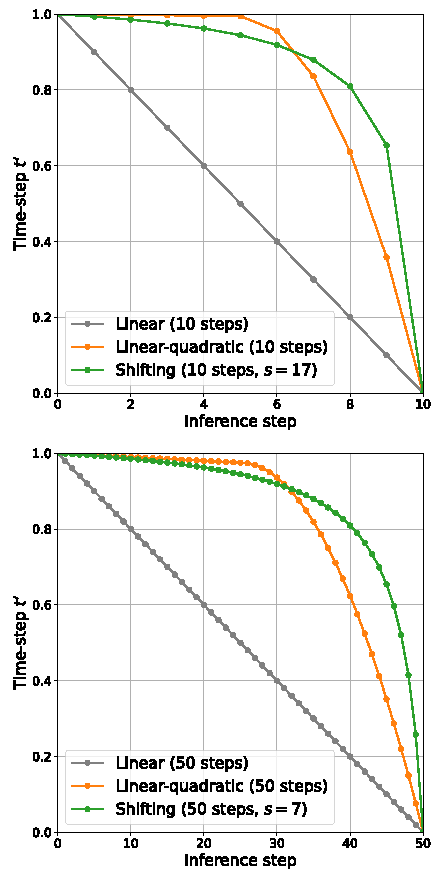
\includegraphics[width=\textwidth]{figures/shifting.pdf}
        \caption{}
        \label{fig:shifting}
    \end{subfigure}
    \hfill
    \begin{subfigure}[b]{0.69\textwidth} % 右边的子图占40%
        \centering
        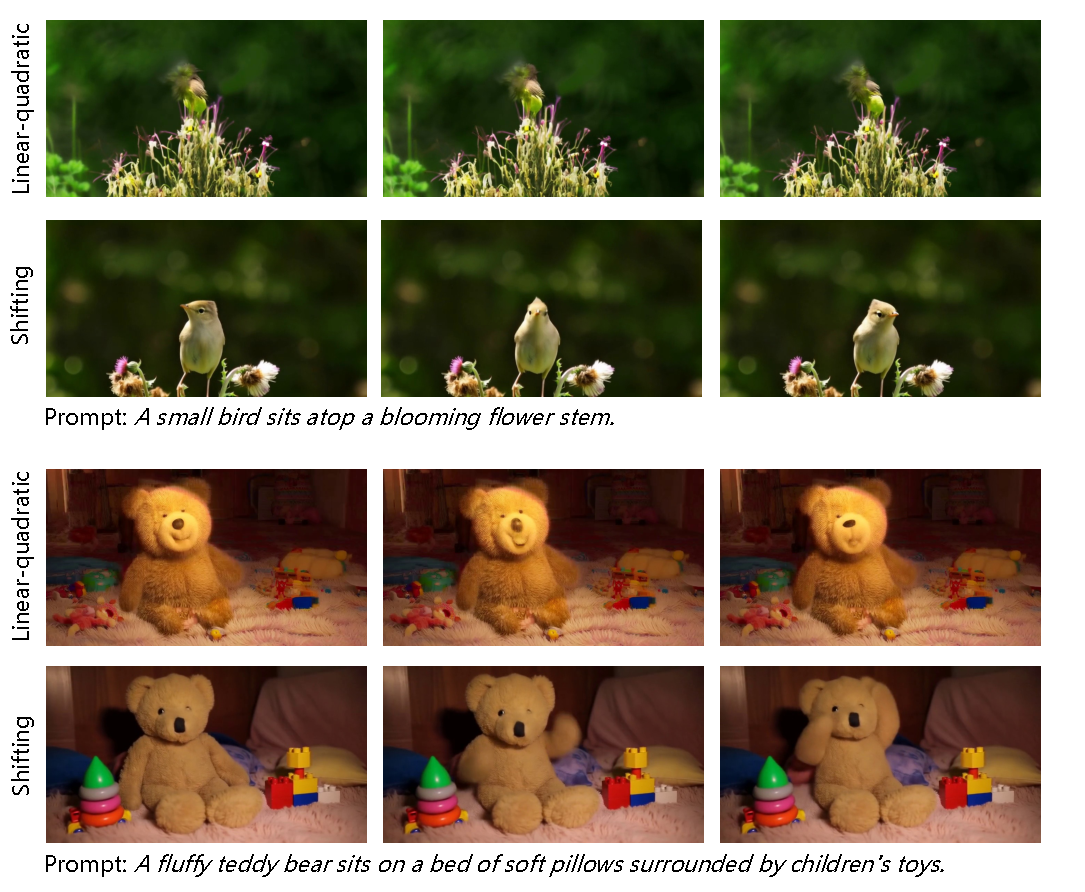
\includegraphics[width=\textwidth]{figures/shifting_example.pdf}
        \caption{}
        \label{fig:shifting_example}
    \end{subfigure}
    \caption{(a) Different time-step schedulers. For our shifting stragty, we set a larger shifting factor $s$ for a lower inference step. (b) Generated videos with only 10 inference steps. The shifting stragty leads to significantly better visual quality.}
    \label{fig:overall}
\end{figure}


\subsection{Inference Step Reduction }
% \dq{@Common Utility Team}

To improve the inference efficiency, we firstly consider reducing the number of inference steps. Compared to image generation, it is more challenging to maintain the spatial and temporal quality of the generated videos with lower inference steps. Inspired by a previous observation that the first time-steps contribute to most changes during the generation process \cite{zhao2024real,polyak2024movie,zhang2022unsupervised,zhang2023shiftddpms}, we utilize the time-step shifting to handle the case of lower inference steps. Specifically, given the inference step $q \in \{1,2,...,Q\}$, $t=1-\frac{q}{Q}$ is the input time condition for the generation model, where the noise is initialized at $t=1$ and the generation process halts at $t=0$. Instead of using $t$ directly, we map $t$ to $t'$ with a shifting function $t'=\frac{s*t}{1+(s-1)*t}$, where $t'$ is the input time condition and $s$ is the shifting factor. If $s>1$, the flow model is conditioned more on early time steps. A critical observation is that a lower inference step requires a larger shifting factor $s$. Empirically, $s$ is set as 7 for 50 inference steps, while $s$ should be increased to 17 when the number of inference steps is smaller than 20. The time-step shifting strategy enables the generation model to match the results of numerous inference steps with a reduced number of steps.

MovieGen \cite{polyak2024movie} applies the linear-quadratic scheduler to achieve a similar goal. The schedulers are visualized in Figure \ref{fig:shifting}. However, we find that our time-step shifting is more effective than the linear-quadratic scheduler in the case of extremely low number of inference steps, $e.g.$, 10 steps. As shown in Figure \ref{fig:shifting_example}, the linear-quadratic scheduler results in worse visual quality. 
 

\subsection{Text-guidance Distillation}
% \dq{@Common Utility Team}

Classifier-free guidance (CFG) \cite{ho2022classifier} significantly improves the sample quality and motion stability of text-conditioned diffusion models.
%However, it increases computational cost and inference latency since it computes the output for the unconditional input except for the conditional one at each inference step.
However, it increases computational cost and inference latency since it requires extra output for the unconditional input at each inference step.
%Generally, the unconditional and conditional inferences are implemented in a single batch in parallel.
Especially for the large video model and high-resolution video generation, the inference burden is extremely expensive when generating text-conditional and text-unconditional videos, simultaneously.
%Due to the great number of parameters and long-context lengths for our video generation model, the need for additional computation and memory becomes more notable. 
To solve this limitation, we distill the combined output for unconditional and conditional inputs into a single student model \cite{meng2023distillation}.
Specifically, the student model is conditioned on a guidance scale and shares the same structures and hyper-parameters as the teacher model.
We initialize the student model with the same parameters as the teacher model and train with the guidance scale randomly sampled from 1 to 8. We experimentally find that text-guidance distillation approximatively brings 1.9x acceleration. 

\subsection{Efficient and Scalable Training}
% \dq{@Infra Team}

% \subsubsection{Overview}
To achieve scalability and efficient training, 
we train \nameofmethod{} on AngelPTM \cite{nie2023angel}, 
the large-scale pretraining framework from Tencent Angel machine learning team.
In this part, we first outline the hardware and infrastructure used for training, and then give a detailed introduction to the model parallel method and its optimization methods, followed by the automatic fault tolerance mechanism.

\subsubsection{Hardware Infrastucture}
% \nameofmethod{} uses NVIDIA GPUs to complete the entire training pipeline.
To ensure efficient communication in large-scale distributed training, we setup a dedicated distributed training framework termed Tencent XingMai network \cite{2024tccl} for highly efficient inter-server communication. 
The GPU scheduling for all training tasks is completed through the Tencent Angel machine learning platform, which provides powerful resource management and scheduling capabilities.

\subsubsection{Parallel Strategy}
\nameofmethod{} training adopts 5D parallel strategies, including tensor parallelism (TP) \cite{2019megatron}, sequence parallelism (SP) \cite{2022sequence-parallelism}, context parallelism (CP) \cite{2024context-parallelism}, and data parallelism combined with Zero optimization (DP + ZeroCache \cite{nie2023angel}).
The tensor parallelism (TP) is based on the principle of block calculation of matrices. The model parameters (tensors) are divided into different GPUs to reduce GPU memory usage and accelerate the calculation. Each GPU is responsible for the calculation of different parts of tensors in the layer.

Sequence parallelism (SP) is based on TP. The input sequence dimension is sliced to reduce the repeated calculation of operators such as LayerNorm and Dropout, and reduce the storage of the same activations, which effectively reduces the waste of computing resources and GPU memory.
In addition, for input data that does not meet the SP requirements, the engineering equivalent SP Padding capability is supported.

Context parallelism (CP) is sliced in the sequence dimension to support long-sequence training. Each GPU is responsible for calculating the Attention of different sequence slices. Specifically, Ring Attention \cite{2023ring-attention} is used to achieve efficient training of long sequences through multiple GPUs, breaking through the GPU memory limitation of a single GPU.

In addition, data parallelism + ZeroCache is leveraged to support horizontal expansion through data parallelism to meet the demand for increasing training data sets. Then, based on data parallelism, the ZeroCache optimization strategy is used to further reduce the redundancy of model states (model parameters, gradients, and optimizer states), and we unify the use of GPU memory to maximize the GPU memory usage efficiency.

\subsubsection{Optimization}
\textbf{Attention optimization.} 
As the sequence length increases, the attention calculation becomes the main bottleneck of training. We accelerated the attention calculation with FusedAttention.

\textbf{Recomputation and activations offload optimization.} Recomputation is a technology that trade calculations for storage. 
It is mainly made up of three parts: a) specifying certain layers or blocks for recalculation, b) releasing the activations in the forward calculation, and c) obtaining the dependent activations through recalculation in the backward calculation, which significantly reduces the use of GPU memory during training.
In addition, considering the PCIe bandwidth and the host memory size, a layer-based activation offload strategy is adopted. Without reducing the training performance, the activations in the GPU memory are offloaded to the host memory, further saving GPU memory.

\subsubsection{Automatic fault tolerance}
In terms of the large-scale training stability of \nameofmethod{}, an automatic fault tolerance mechanism is used to quickly restore training for common hardware failures.
This avoids frequent occurrence of the manual recovery of training tasks.
%, which  due to failure to the recovery of the training task is in minutes.
By automatically detecting errors and quickly replacing healthy nodes to pull up training tasks, the training stability is 99.5\%.



\section{Fundation Model Performance}
\label{sec:exp}

\myPara{Text Alignment}
% \dq{@Tianqi, Weijie, Daquan}
One of the key metrics for video generative models is their ability to follow text prompts accurately. This capability is essential for the effectiveness of these models. However, some open-source models often struggle to capture all subjects or accurately represent the relationships between multiple subjects, particularly when the input text prompt is complex.
%
\nameofmethod{} demonstrates robust capabilities in generating videos that closely adhere to the provided text prompts. As illustrated in Figure \ref{fig:text-align}, it effectively manages multiple subjects within the scene.

\begin{figure}[h]
    \centering
    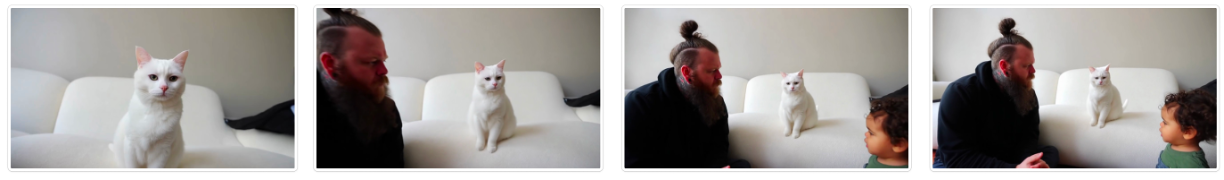
\includegraphics[width=\linewidth]{figures/text_alignment.png}
    \caption{{Prompt: A white cat sits on a white soft sofa like a person, while its long-haired male owner, with his hair tied up in a topknot, sits on the floor, gazing into the cat's eyes. His child stands nearby, observing the interaction between the cat and the man. } }
    \label{fig:text-align}
\end{figure}


\myPara{High-quality}
% \dq{@Jodai}
We also perform a fine-tuning process to enhance the spatial quality of the generated videos. As illustrated in Figure \ref{fig:high_quality}, \nameofmethod{} is capable of producing videos with ultra-detailed content.
\begin{figure}[!htbp]
    \centering
    \begin{subfigure}{\textwidth}
        \centering
        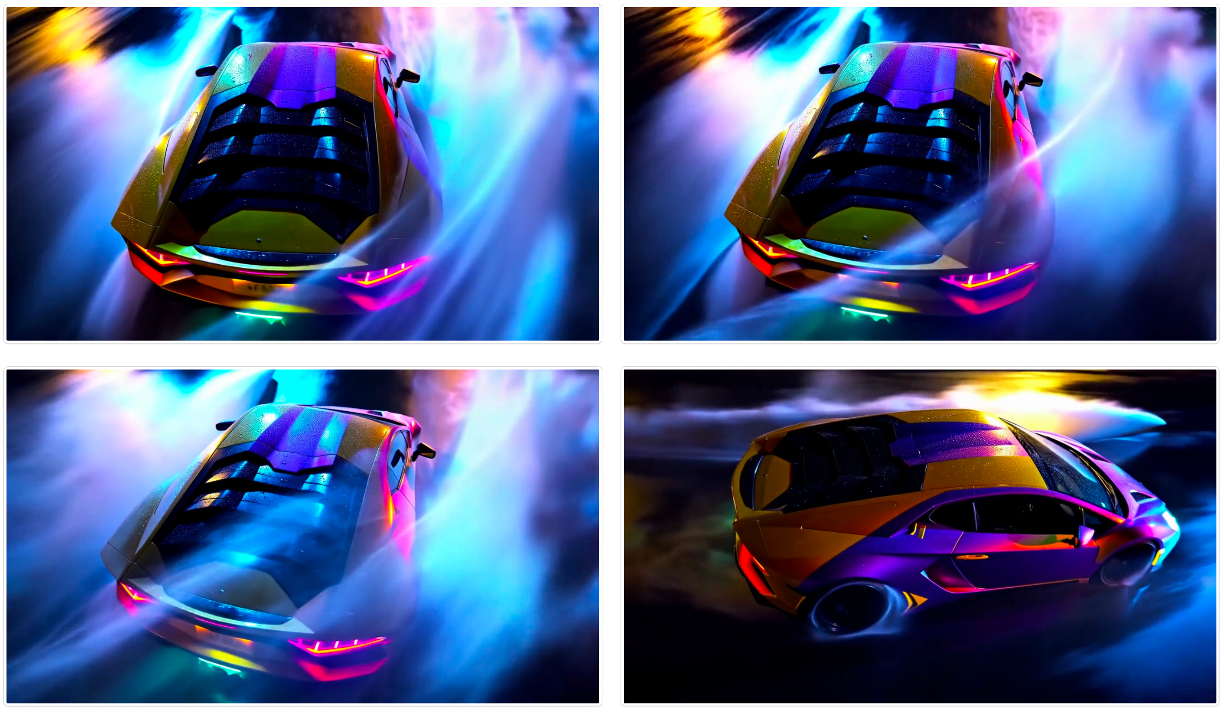
\includegraphics[width=\textwidth]{figures/high-quality-1.png}
        \caption{Prompt: the ultra-wide-angle lens follows closely from the hood, with raindrops continuously splattering against the lens. Ahead, a sports car speeds around a corner, its tires violently skidding against the wet road, creating a mist of water. Neon lights refract in the rain, leaving colorful streaks on the car's surface. The camera swiftly shifts to the side of the car, capturing the wheels spinning at high speed, before finally moving to the rear.}
    \end{subfigure}
    \hfill
    \begin{subfigure}{\textwidth}
        \centering
        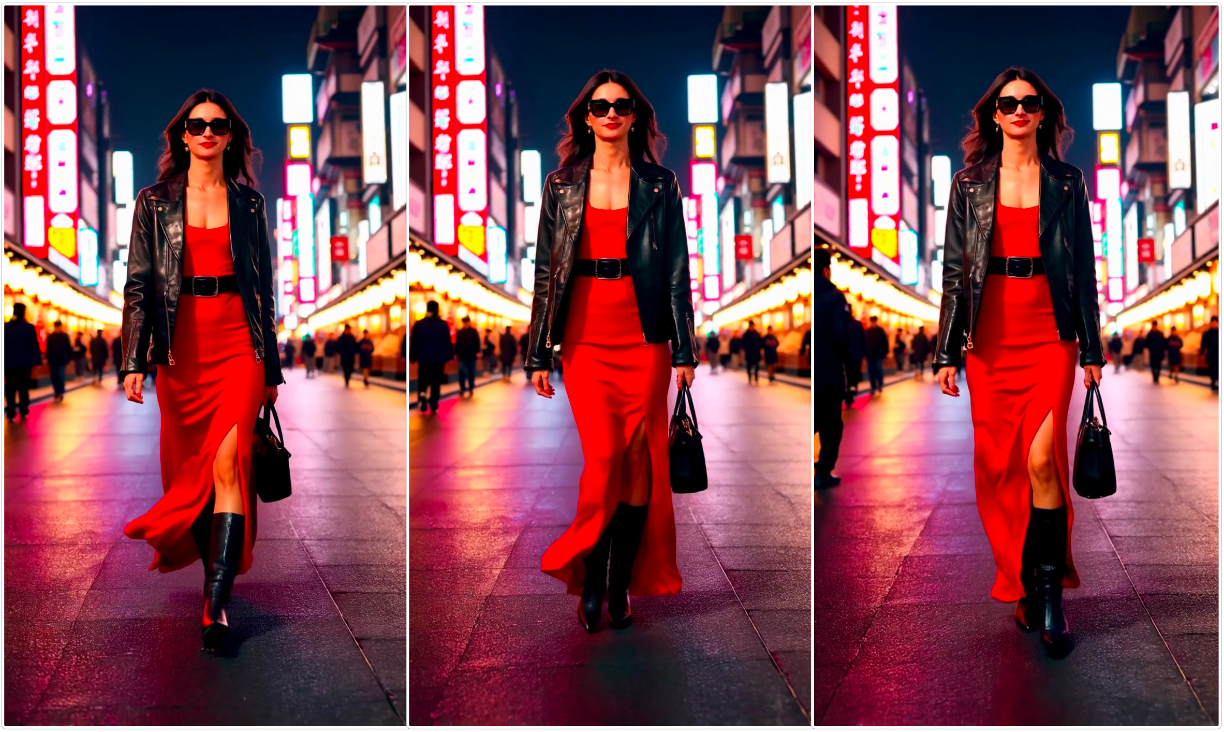
\includegraphics[width=\textwidth]{figures/high-quality-2.png}
        \caption{Prompt: a stylish woman walks down a Tokyo street filled with warm glowing neon and animated city signage. She wears a black leather jacket, a long red dress, and black boots, and carries a black purse. She wears sunglasses and red lipstick. She walks confidently and casually. The street is damp and reflective, creating a mirror effect of the colorful lights. Many pedestrians walk about.}
    \end{subfigure}
    \caption{High-quality videos generated by HunyuanVideo.}
    \label{fig:high_quality}
\end{figure}

\myPara{High-motion Dynamics}
% \dq{@Weijie, Junkun}
In this part, we demonstrate \nameofmethod{}'s capabilities in producing high-dynamic videos based on given prompts. As shown in Figure \ref{fig:high_motion}, our model excels in generating videos that encompass a wide range of scenes and various types of motion.

\begin{figure}[!htbp]
    \centering
    \begin{subfigure}{\textwidth}
        \centering
        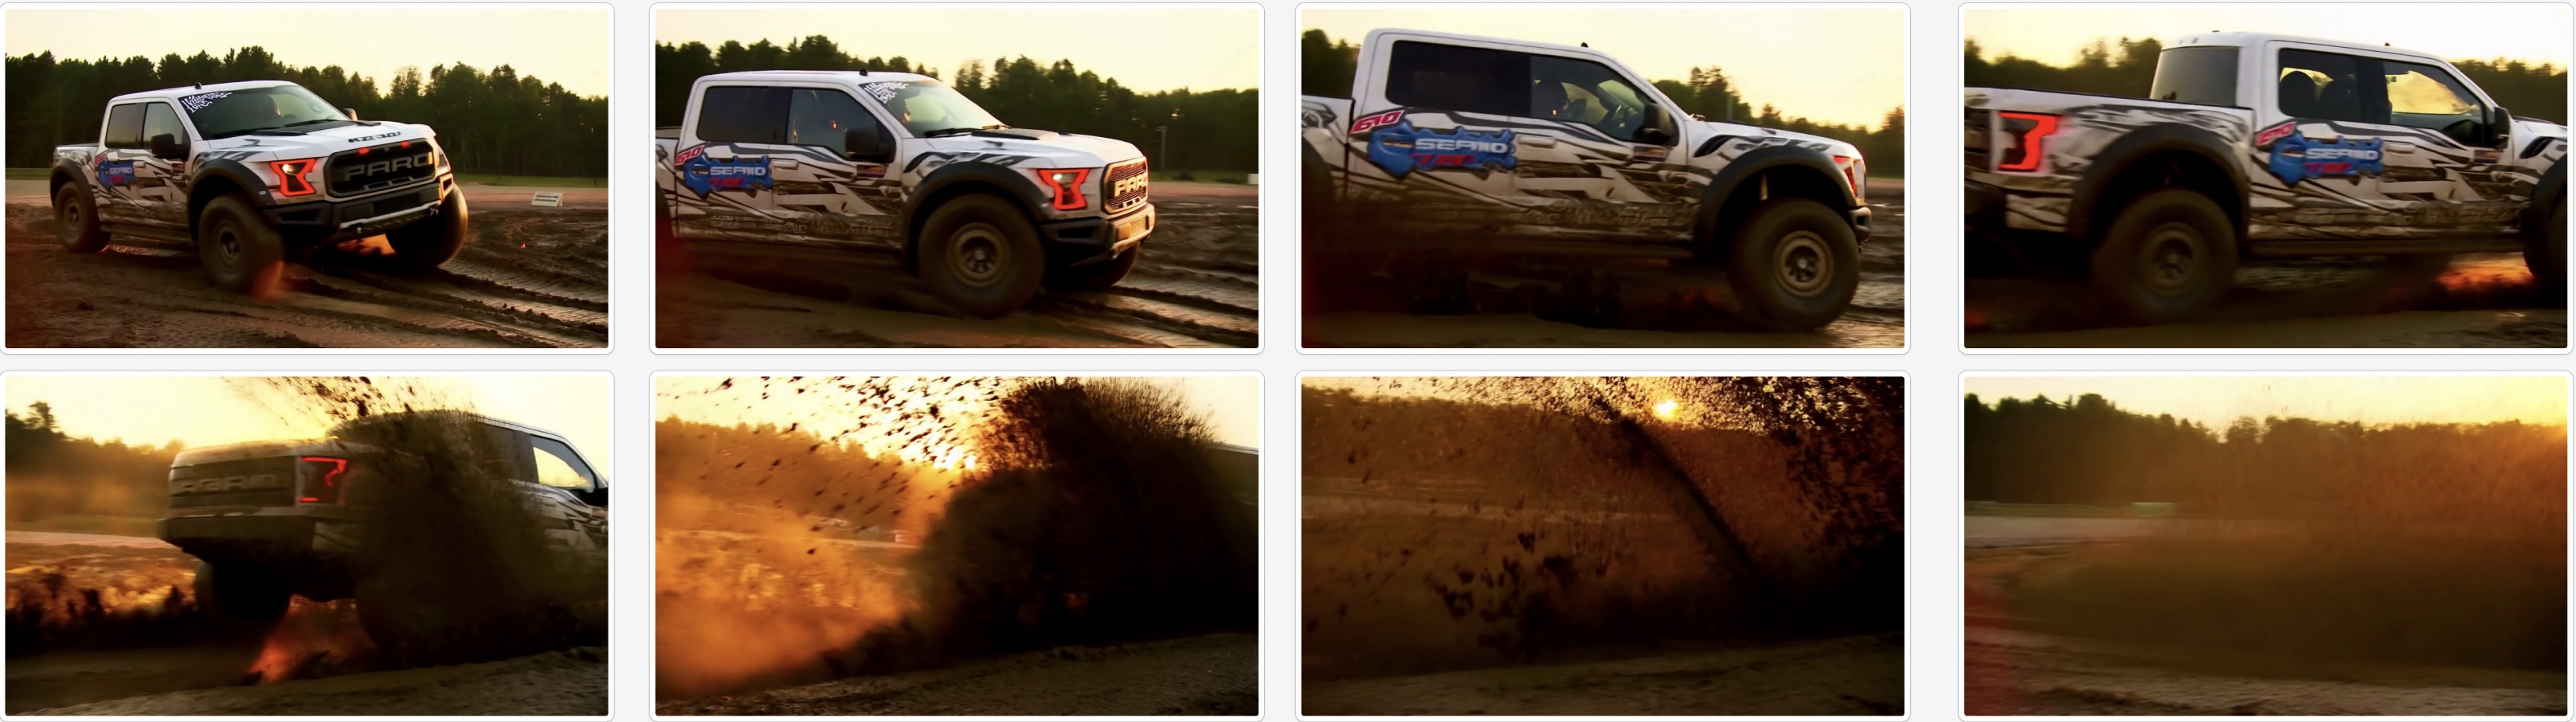
\includegraphics[width=\textwidth]{figures/high_motion_3.jpg}
        \captionsetup{font=small}
        \caption{Prompt: At sunset, a modified Ford F-150 Raptor roared past on the off-road track. The raised suspension allowed the huge explosion-proof tires to flip freely on the mud, and the mud splashed on the roll cage.}
        \label{fig:hm_1}
    \end{subfigure}
    \hfill
    \begin{subfigure}{\textwidth}
        \centering
        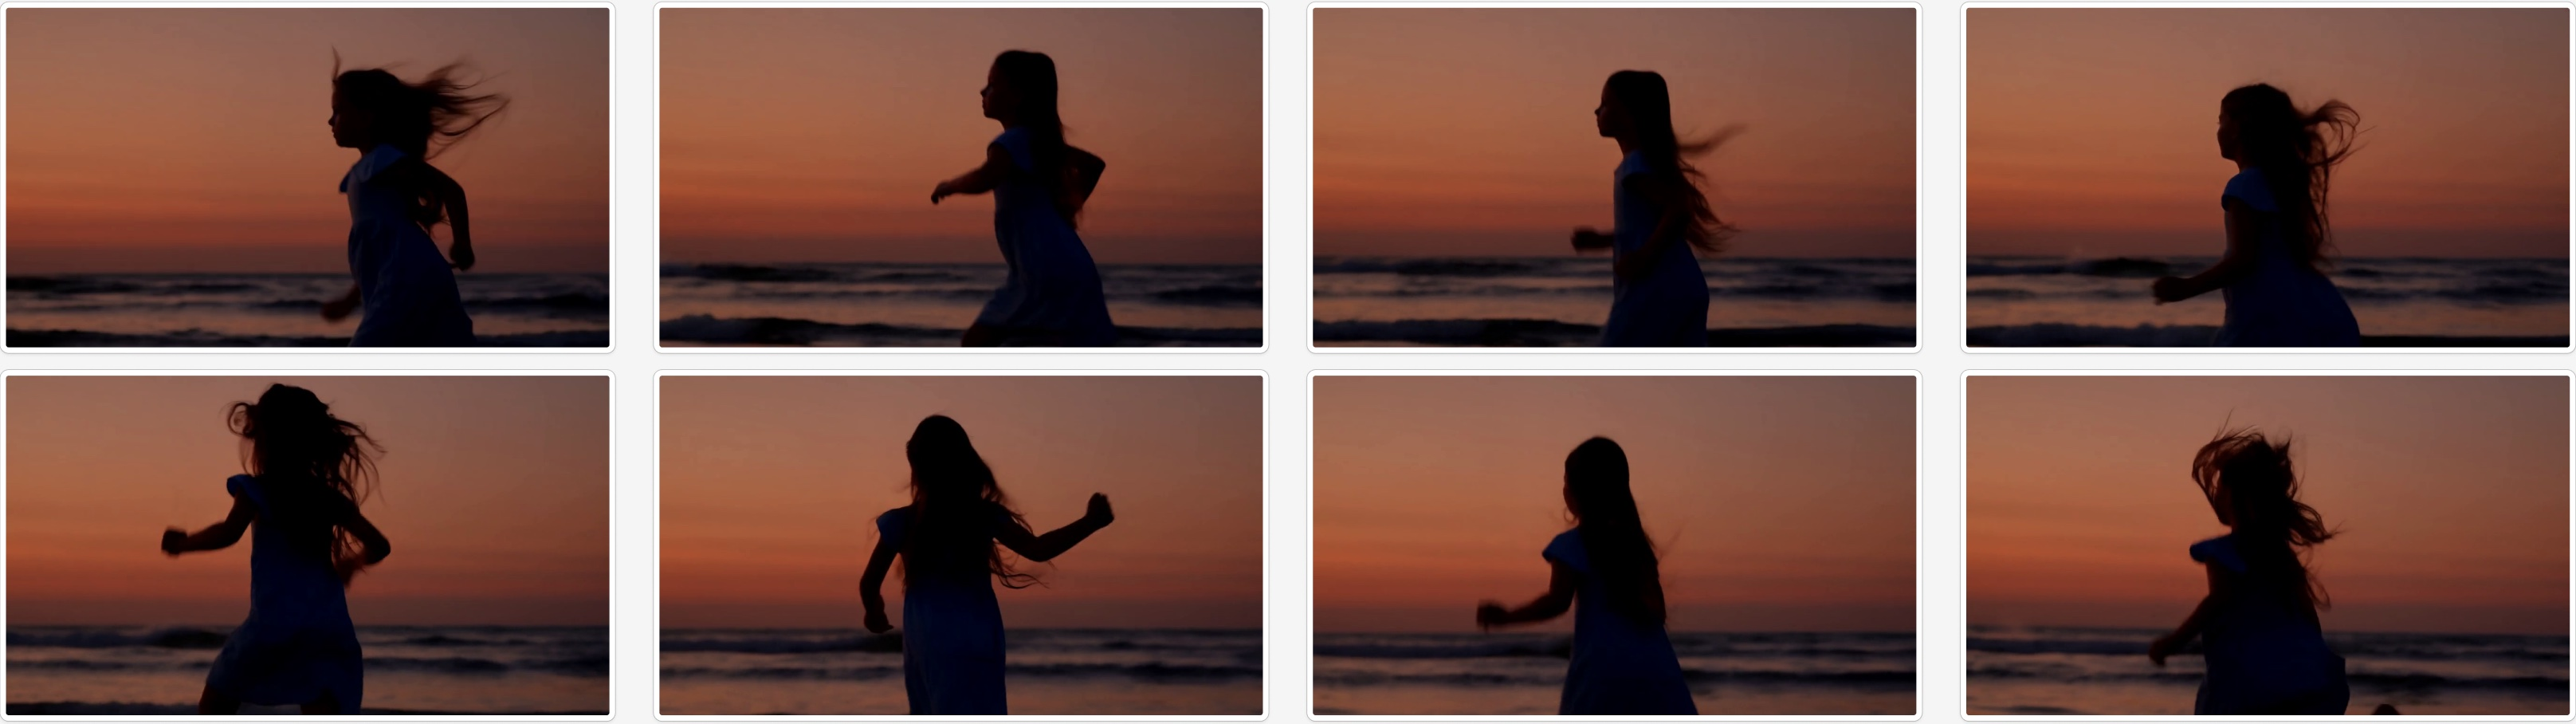
\includegraphics[width=\textwidth]{figures/high_motion_5.jpg}
        \captionsetup{font=small}
        \caption{Prompt: The panning camera moves forward slowly, with a depth of field in the middle focus, and warm sunset light covers the screen. The girl in the picture runs with her skirt fluttering, turns and jumps.}
        \label{fig:hm_2}
    \end{subfigure}
    \hfill
    \begin{subfigure}{\textwidth}
        \centering
        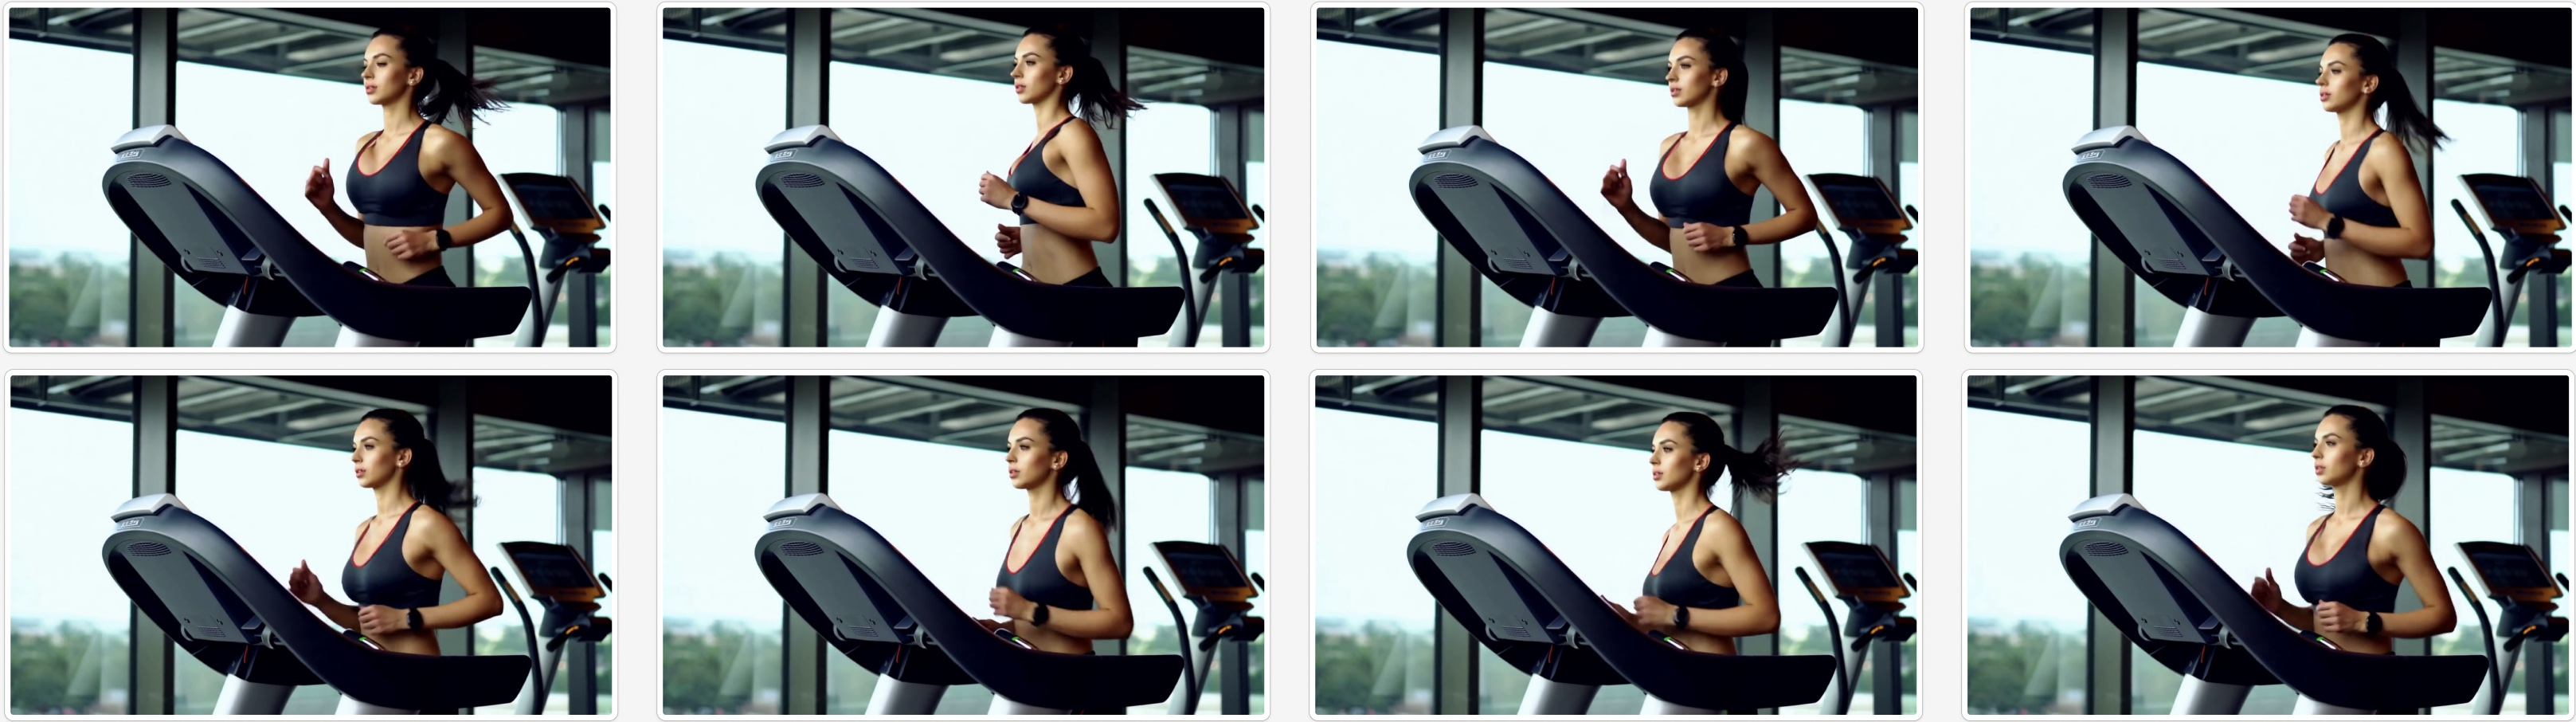
\includegraphics[width=\textwidth]{figures/high_motion_2.jpg}
        \captionsetup{font=small}
        \caption{Prompt: In the gym, a woman in workout clothes runs on a treadmill. Side angle. Realistic, Indoor lighting, Professional.}
        \label{fig:hm_3}
    \end{subfigure}
    \hfill
    \begin{subfigure}{\textwidth}
        \centering
        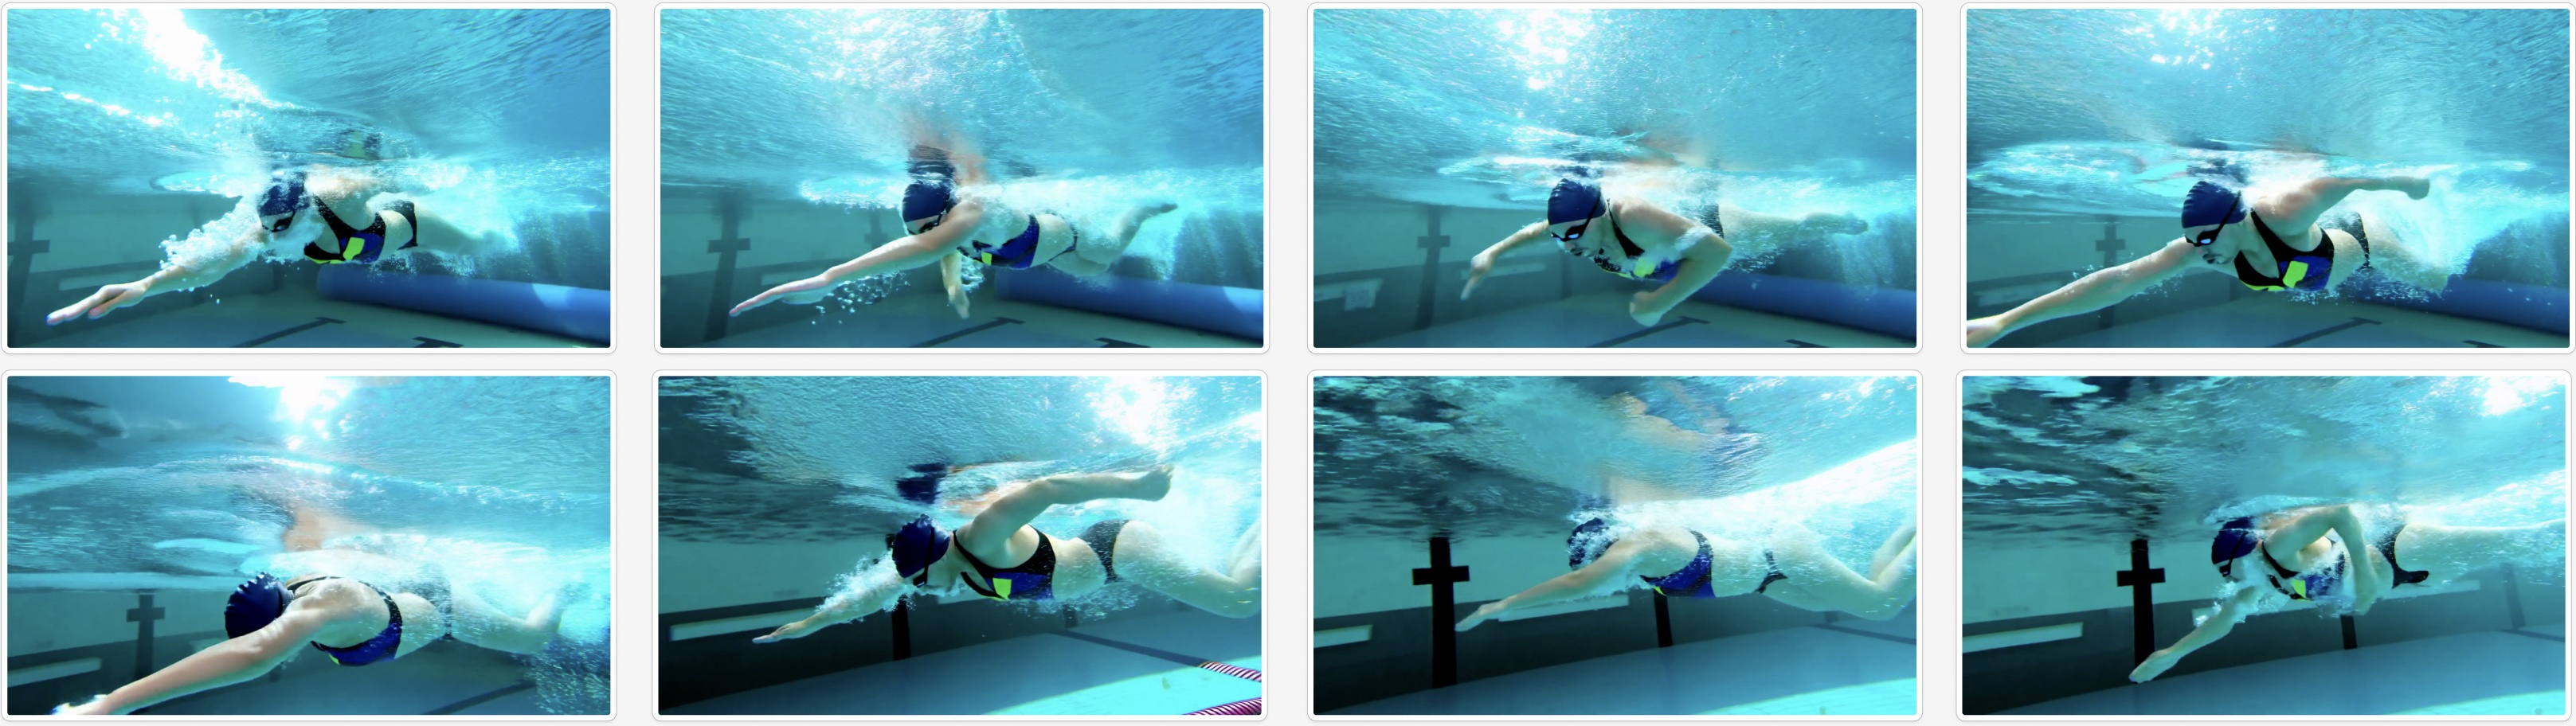
\includegraphics[width=\textwidth]{figures/high_motion_7.jpg}
        \captionsetup{font=small}
        \caption{Prompt: Swimmer swimming underwater, in slow motion. Realistic, Underwater lighting, Peaceful.}
        \label{fig:hm_4}
    \end{subfigure}
    \hfill
    \begin{subfigure}{\textwidth}
        \centering
        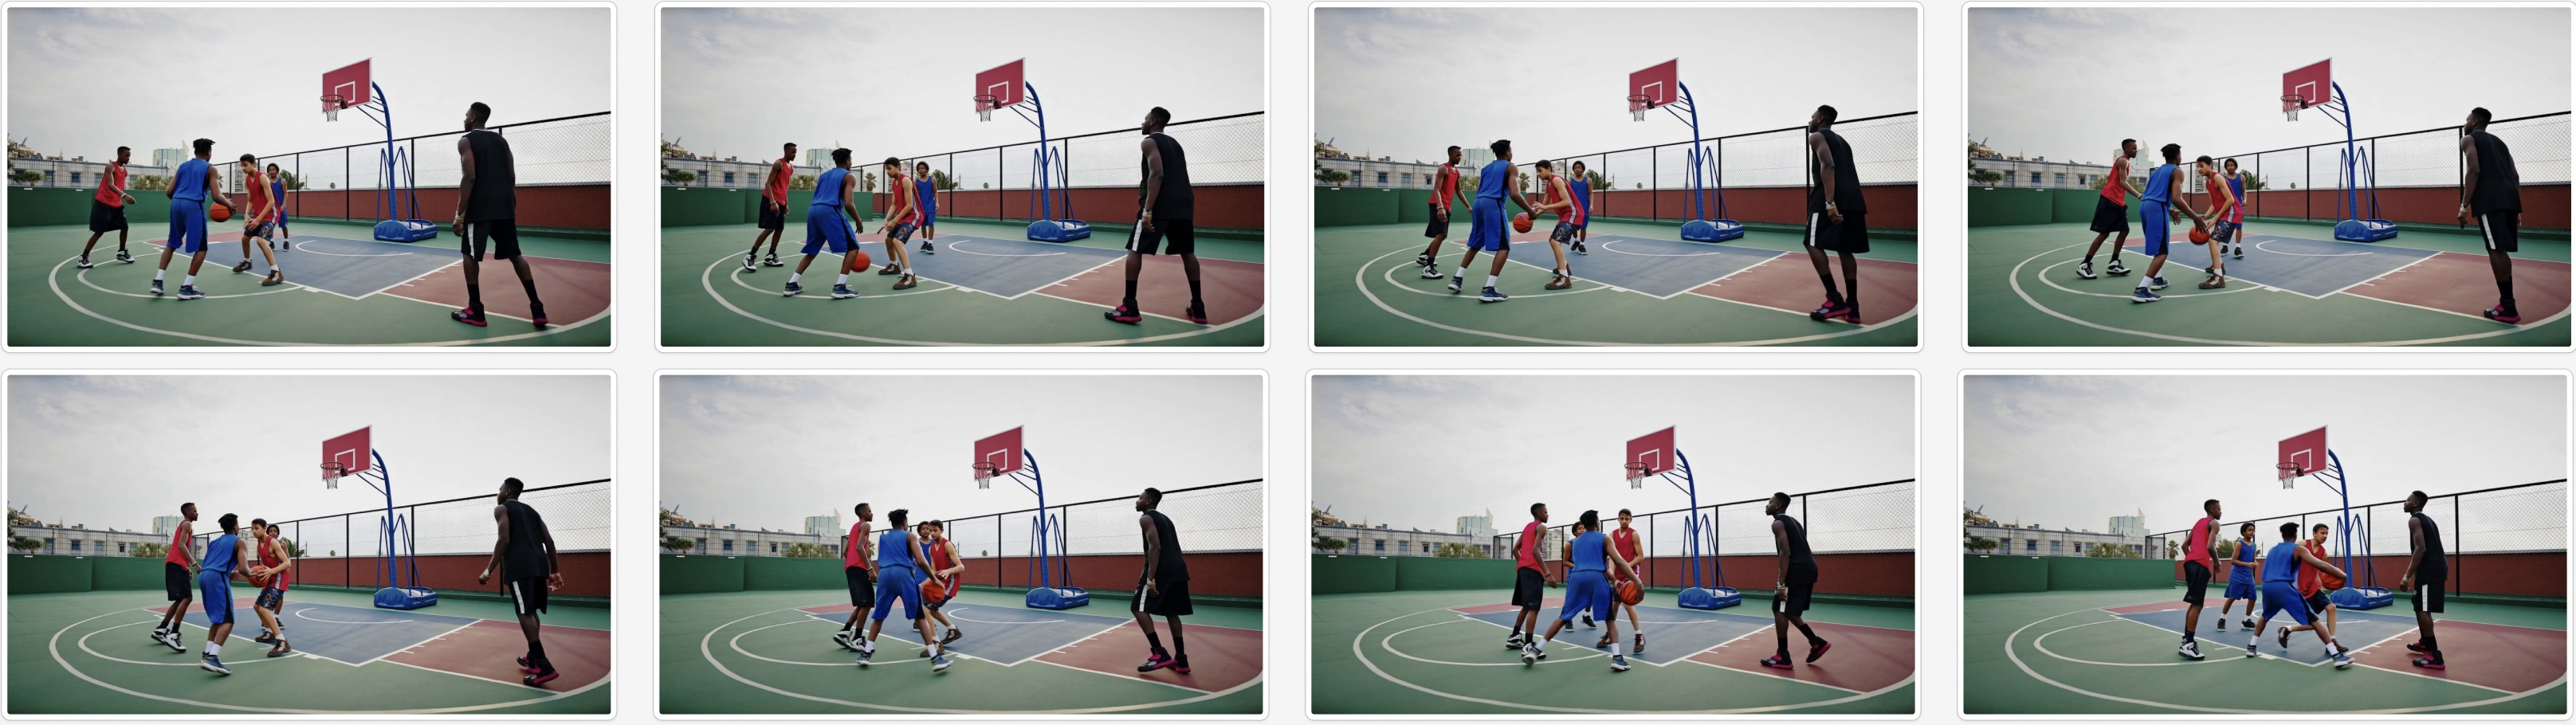
\includegraphics[width=\textwidth]{figures/high_motion_8.jpg}
        \captionsetup{font=small}
        \caption{Prompt: On the rooftop, there is an open-air basketball court, and five male students are playing basketball. Realistic, Natural lighting, Casual.}
        \label{fig:hm_5}
    \end{subfigure}
    \caption{High-motion dynamics videos generated by \nameofmethod{}.}
    \label{fig:high_motion}
\end{figure}


\myPara{Concept Generalization}
% \dq{@Daquan, Zhiyu}
One of the most desirable features of a generative model is its ability to generalize concepts. As illustrated in Figure \ref{fig:concept}, the text prompt describes a scene: "In a distant galaxy, an astronaut floats on a shimmering, pink, gemstone-like lake that reflects the vibrant colors of the surrounding sky, creating a stunning scene. The astronaut gently drifts on the lake's surface, while the soft sounds of water whisper the planet's secrets. He reaches out, his fingertips gliding over the cool, smooth water." Notably, this specific scenario has not been encountered in the training dataset. Furthermore, it is evident that the depicted scene combines several concepts that are also absent from the training data.
\begin{figure}[!htbp]
    \centering
    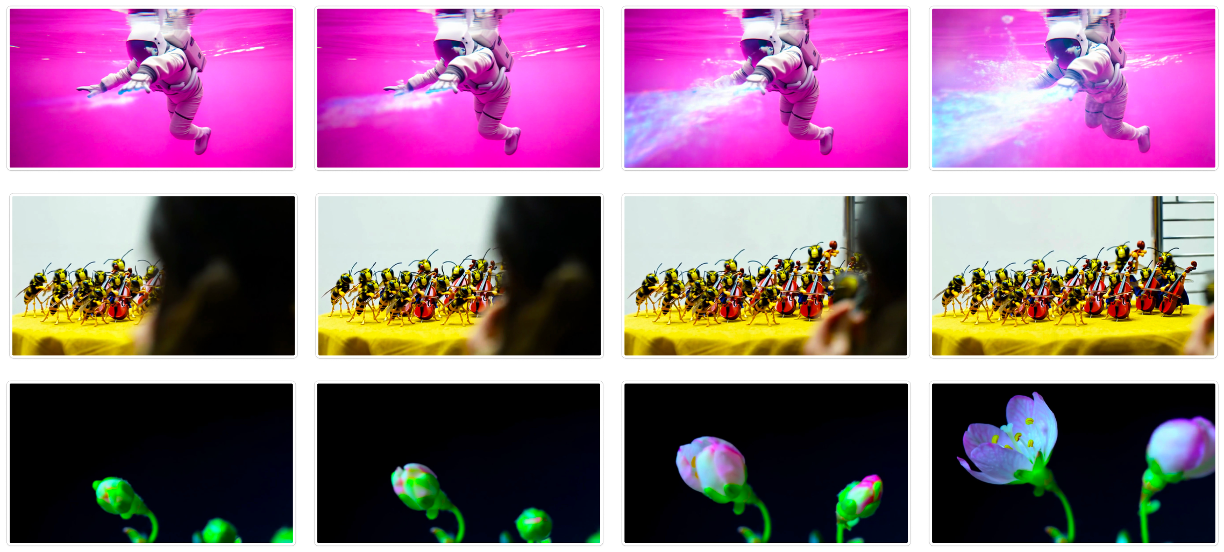
\includegraphics[width=\linewidth]{figures/concept.png}
    \caption{\small {\nameofmethod{}'s performance on concept generalization. The results of the three rows correspond to the text prompts (1) `In a distant galaxy, an astronaut floats on a shimmering, pink, gemstone-like lake that reflects the vibrant colors of the surrounding sky, creating a stunning scene. The astronaut gently drifts on the lake's surface, the soft sounds of water whispering the planet's secrets. He reaches out, his fingertips gliding over the cool, smooth water. ', (2) `A macro lens captures a tiny orchestra of insects playing instruments.' and (3) `The night-blooming cactus flowers in the evening, with a brief, rapid closure. Time-lapse shot, extreme close-up. Realistic, Night lighting, Mysterious.' respectively.} }
    \label{fig:concept}
\end{figure}

\myPara{Action Reasoning and Planning}
% \dq{@Li Xin}
Leveraging the capabilities of large language models, \nameofmethod{} can generate sequential movements based on a provided text prompt. As demonstrated in Figure \ref{fig:sequential-move}, \nameofmethod{} effectively captures all actions in a photorealistic style.
\begin{figure}[ht]
    \centering
    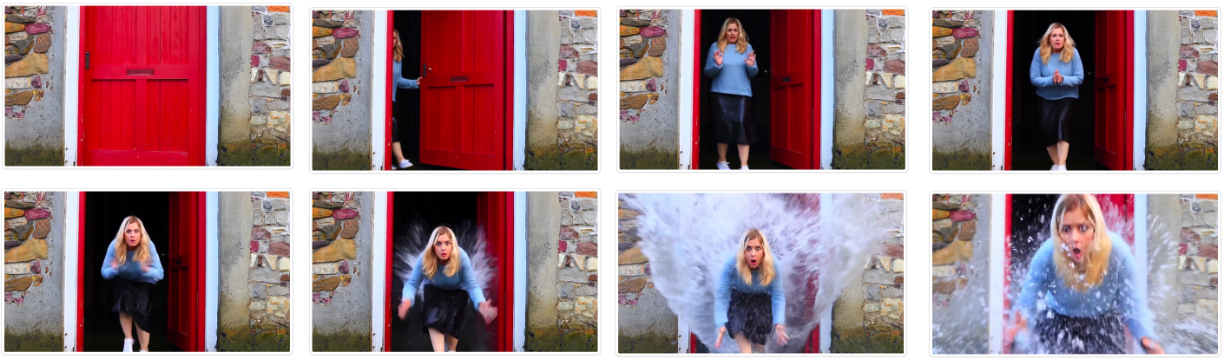
\includegraphics[width=\linewidth]{figures/sequential_motion.png}
    \caption{{Prompt: The woman walks over and opens the red wooden door. As the door swings open, seawater bursts forth, in a realistic style.}}
    \label{fig:sequential-move}
\end{figure}

\myPara{Character Understanding and Writing}
\nameofmethod{} is capable of generating both scene text and gradually appearing handwritten text as shown in Fig.~\ref{fig:ocr}. 



% \dq{@Wuyue}
\begin{figure}[!htbp]
    \centering    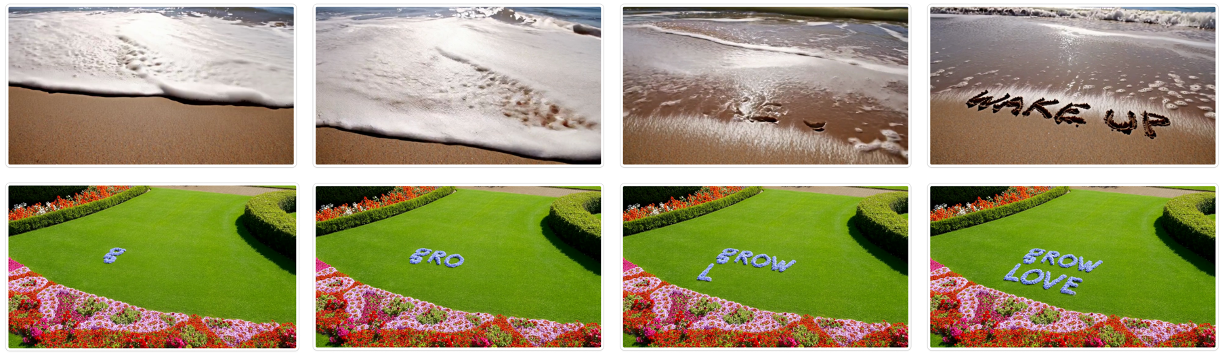
\includegraphics[width=\linewidth]{figures/ocr.png}
    \caption{High text-video alignment videos generated by HunyuanVideo. Top row: Prompt: A close-up of a wave crashing against the beach, the sea foam spells out ``WAKE UP'' on the sand. Bottom row: Prompt: In a garden filled with blooming flowers, ``GROW LOVE'' has been spelled out with colorful petals.}
    \label{fig:ocr}
\end{figure}





\subsection{Comparison with SOTA Models}
To evaluate the performance of \nameofmethod{}, we selected five strong baselines from closed-source video generation models. In total, we utilized 1,533 text prompts, generating an equal number of video samples with \nameofmethod{} in a single run. For a fair comparison, we conducted inference only once, avoiding any cherry-picking of results. When comparing with the baseline methods, we maintained the default settings for all selected models, ensuring consistent video resolution. 60 professional evaluators performed the evaluation and the results are presented in Table \ref{tab:compare}. Videos were assessed based on three criteria: Text Alignment, Motion Quality, and Visual Quality. Notably, \nameofmethod{} demonstrated the best overall performance, particularly excelling in motion quality. We randomly sample 600 videos out of 1533 for public access\footnote{https://github.com/Tencent/HunyuanVideo}.
\begin{table}[h]
    \centering
    \footnotesize
    \caption{Model Performance Evaluation}
    \begin{tabular}{@{}llccccc@{}}
        \toprule
        Model Name                             &  Duration & Text Alignment  & Motion Quality  & Visual Quality  & Overall  & Ranking \\ \midrule
        \nameofmethod{} (Ours)               & 5s       & 61.8\%               & 66.5\%          & 95.7\%          & 41.3\%      & 1              \\
        CNTopA (API)       & 5s       & 62.6\%               & 61.7\%          & 95.6\%          & 37.7\%      & 2              \\
        CNTopB (Web)          & 5s       & 60.1\%               & 62.9\%          & 97.7\%          & 37.5\%      & 3              \\
        GEN-3 alpha (Web)           & 6s       & 47.7\%               & 54.7\%          & 97.5\%          & 27.4\%      & 4              \\
        Luma1.6 (API)                & 5s       & 57.6\%               & 44.2\%          & 94.1\%          & 24.8\%      & 5              \\
        CNTopC (Web)        & 5s       & 48.4\%               & 47.2\%          & 96.3\%          & 24.6\%      & 6              \\
         \bottomrule
    \end{tabular}
    \label{tab:compare}

\end{table}




\section{Applications}
\label{sec:application}

\subsection{Audio Generation based on Video}
% \dq{@yutao, james, miles}

Our video-to-audio(V2A) module is designed to enhance generated video content by incorporating synchronized sound effects and contextually appropriate background music. Within the conventional film production pipeline, Foley sound design constitutes an integral component, significantly contributing to the auditory realism and emotional depth of visual media. However, the creation of Foley audio is both time-intensive and demands a high degree of professional expertise. With the advent of an increasing number of text-to-video (T2V) models, most of them lack the corresponding foley generation capabilities, thereby limiting their ability to produce fully immersive content. Our V2A module addresses this critical gap by autonomously generating cinematic-grade foley audio tailored to the input video and textual prompts, thus enabling the synthesis of a cohesive and holistically engaging multimedia experience.

\subsubsection{Data }
Unlike text-to-video (T2V) models, video-to-audio (V2A) models have different requirements for data. As mentioned above, we constructed a video dataset comprising of video-text pairs. However, not all data in this dataset are suitable for training the V2A model. For example, some videos lack an audio stream, others contain extensive voice-over content or their ambient audio tracks have been removed and replaced with unrelated elements. To address these challenges and ensure data quality, we designed a robust data filtering pipeline specifically tailored for V2A training.

First, we filter out videos without audio streams or those in which the silence ratio exceeds 80\%. Next, we employ a frame-level audio detection model, like \cite{Hung2022}, to detect speech, music, and general sound in the audio stream. Based on this analysis, we classify the data into four distinct categories: \textit{pure sound}, \textit{sound with speech}, \textit{sound with music}, and \textit{pure music}. Subsequently, to prioritize high-quality data, we train a model inspired by CAVP \cite{luo2024diff} to compute a visual-audio consistency score, which quantifies the alignment between the visual and auditory components of each video. Using this scoring system in conjunction with the audio category labels, we systematically sample portions of data from each category, retaining approximately 250,000 hours from the original dataset for pre-training. For the supervised fine-tuning stage, we further refine our selection, curating a subset of millions of high-quality clips~(80,000 hours).

For feature extraction, we use CLIP \cite{clip} to obtain visual features at a temporal resolution of 4 fps and subsequently resample these features to align with the audio frame rate. To generate captions, we employ \cite{haji2024taming} as the sound captioning model and \cite{doh2023lp} as the music captioning model. When both sound and music captions are available, we merge them into a structured caption format, following the approach detailed in \cite{polyak2024movie}.

\subsubsection{Model}
Just like the above-mentioned text-to-video model, our video-to-audio generation model also adopts a flow-matching-based diffusion transformer (DiT) as its architectural backbone. The detailed design of the model is depicted in Figure \ref{fig:audio-gen}, illustrating a transition from a triple-stream structure to a single-stream DiT framework.

The model operates within a latent space encoded by a variational autoencoder (VAE) trained on mel-spectrograms. Specifically, the audio waveform is first converted into a 2D mel-spectrogram representation. This spectrogram is subsequently encoded into a latent space using a pretrained VAE. For feature extraction, we leverage pretrained CLIP \cite{clip} and T5 \cite{raffel2020exploring} encoders to independently extract visual and textual features, respectively. These features are subsequently projected into the DiT-compatible latent space using independent linear projections followed by SwiGLU activation, as depicted in Figure \ref{fig:audio-gen}.

To effectively integrate multimodal information, we incorporate stacked triple-stream transformer blocks, which independently process visual, audio, and textual modalities. These are later followed by single-stream transformer blocks to ensure seamless fusion and alignment across modalities. This design enhances the alignment between audio-video and audio-text representations, facilitating improved multimodal coherence.

Once the latent representation is generated by the diffusion transformer, the VAE decoder reconstructs the corresponding mel-spectrogram. Finally, the mel-spectrogram is converted back into an audio waveform using a pre-trained HifiGAN vocoder \cite{kong2020hifi}. This framework ensures a high-fidelity reconstruction of audio signals while maintaining strong multimodal alignment.

\begin{figure}[t]
    \centering
    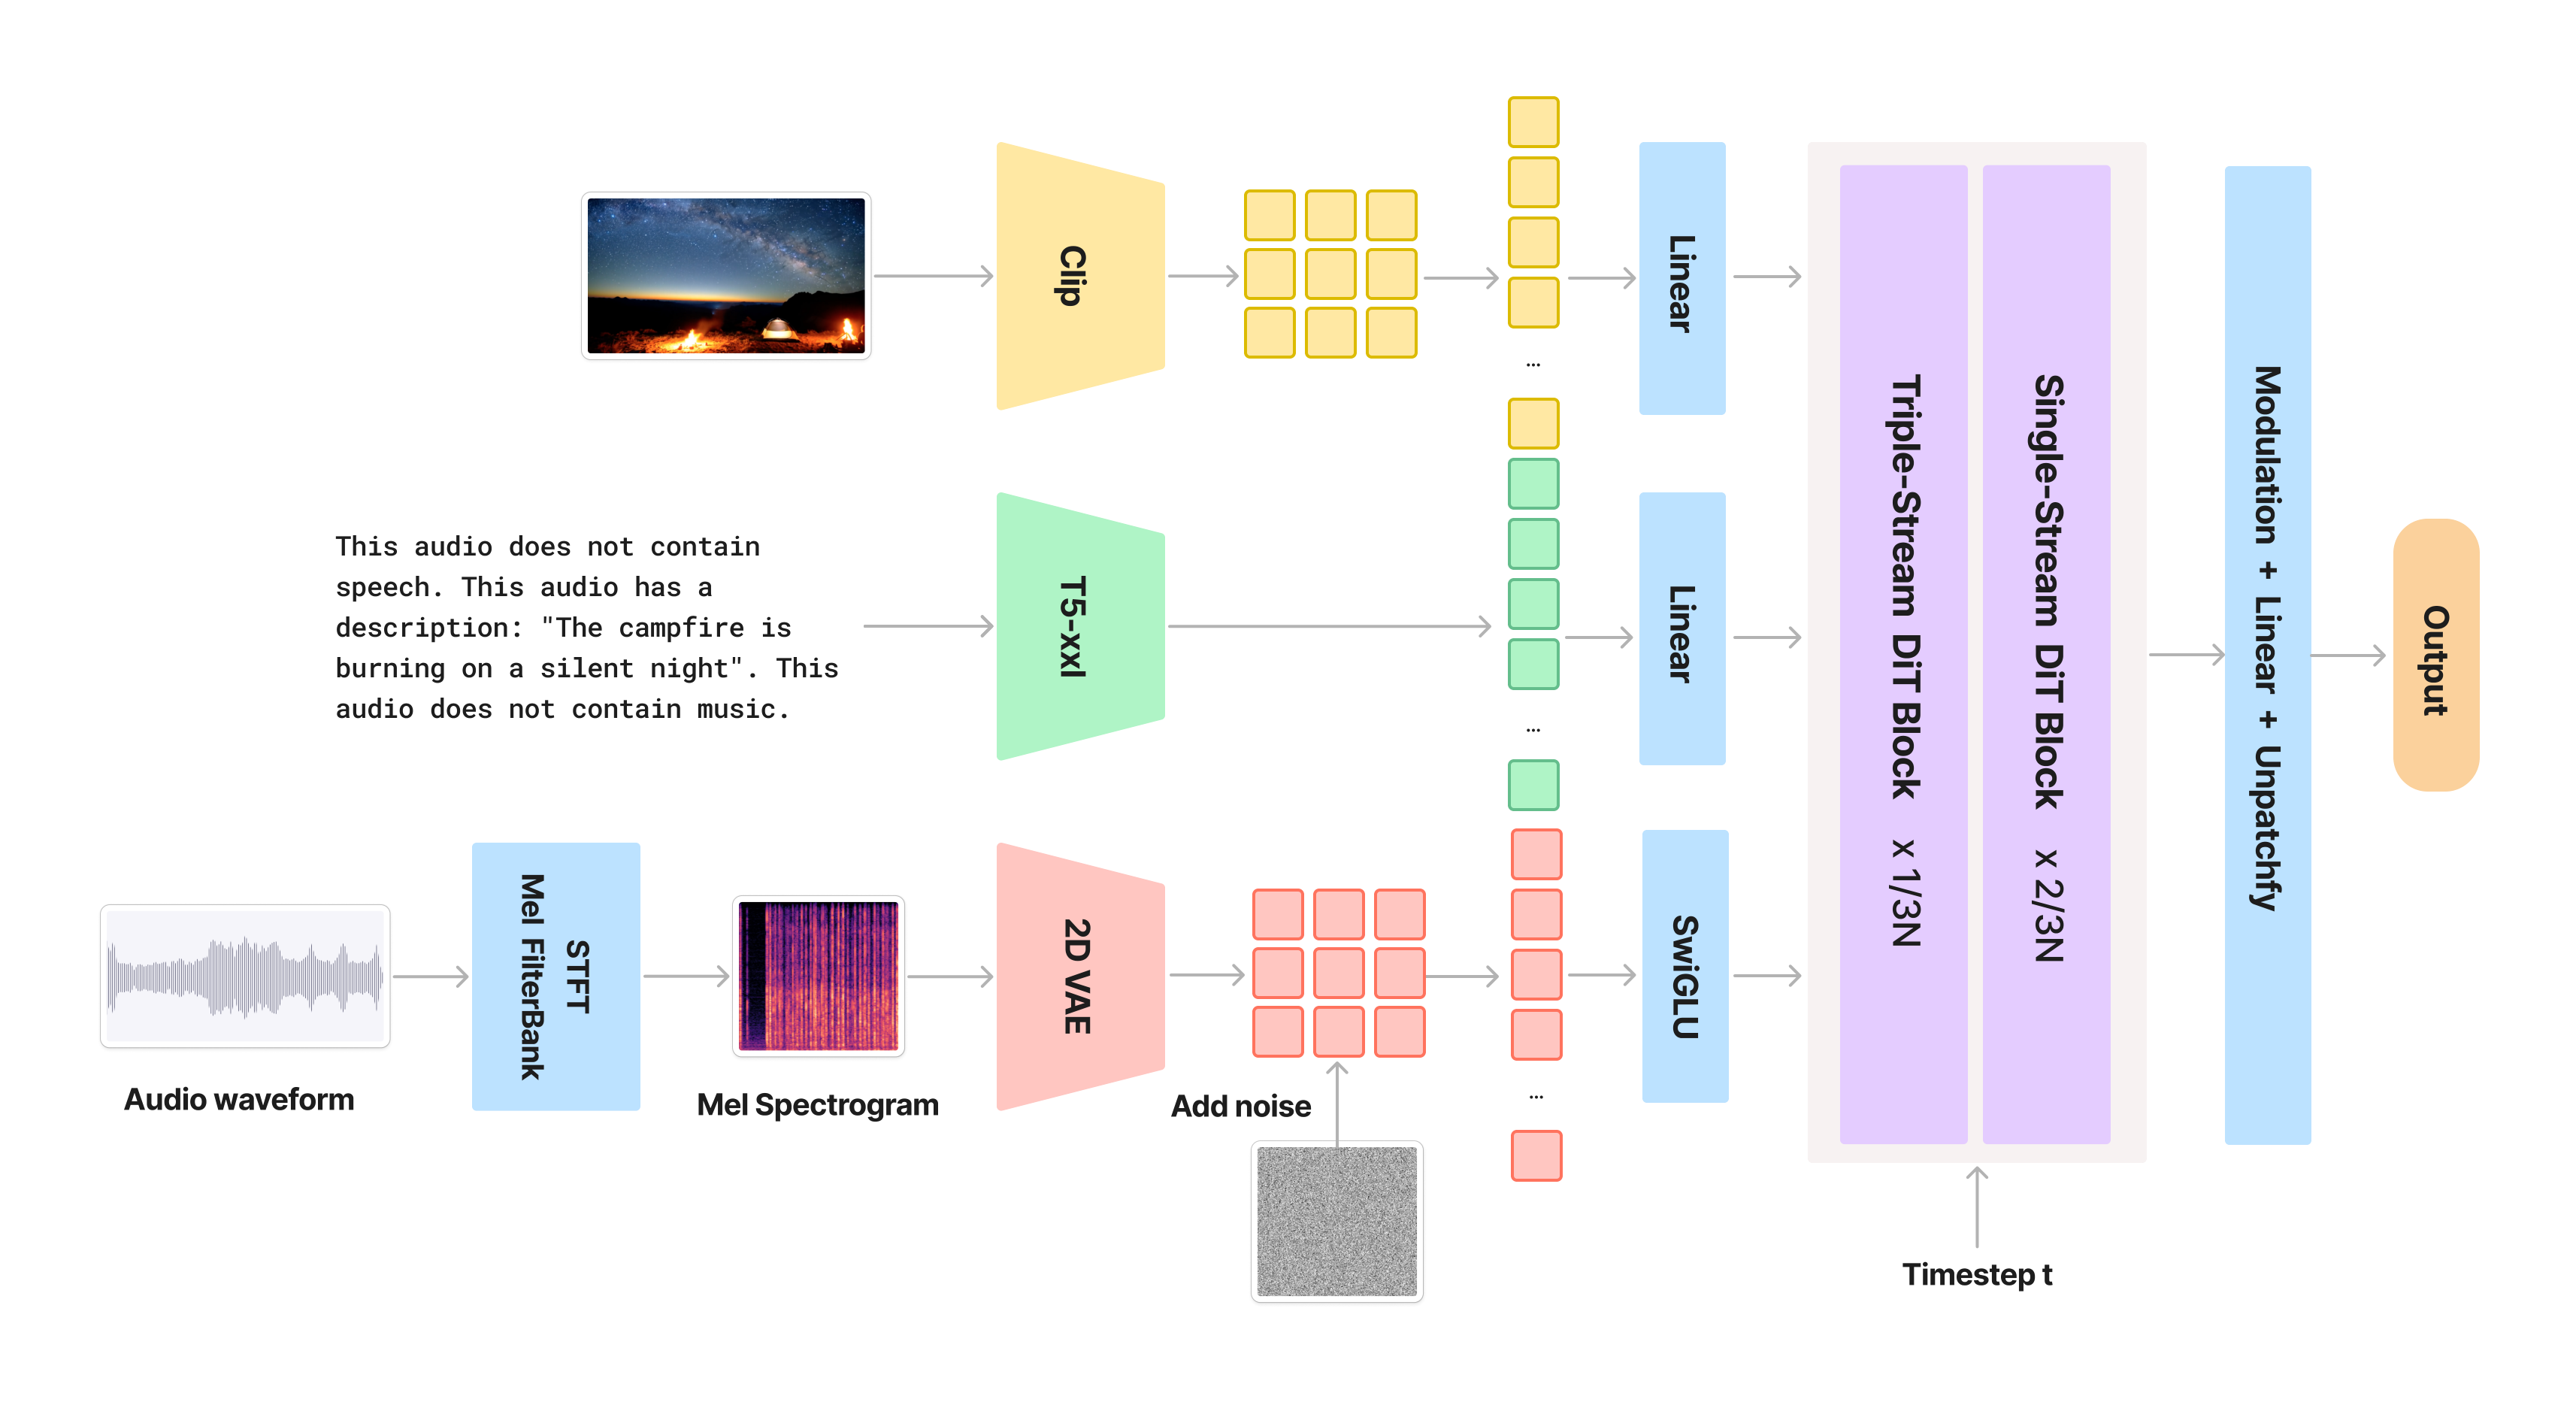
\includegraphics[width=0.9\linewidth]{figures/vt2a_arch.png}
    \caption{The architecture of sound effect and music generation model. }
    \label{fig:audio-gen}
\end{figure}


\subsection{Hunyuan Image-to-Video}
% \dq{Tianqi, Weijie, Daquan}
\subsubsection{Pre-training}
\begin{figure}[t]
    \centering
    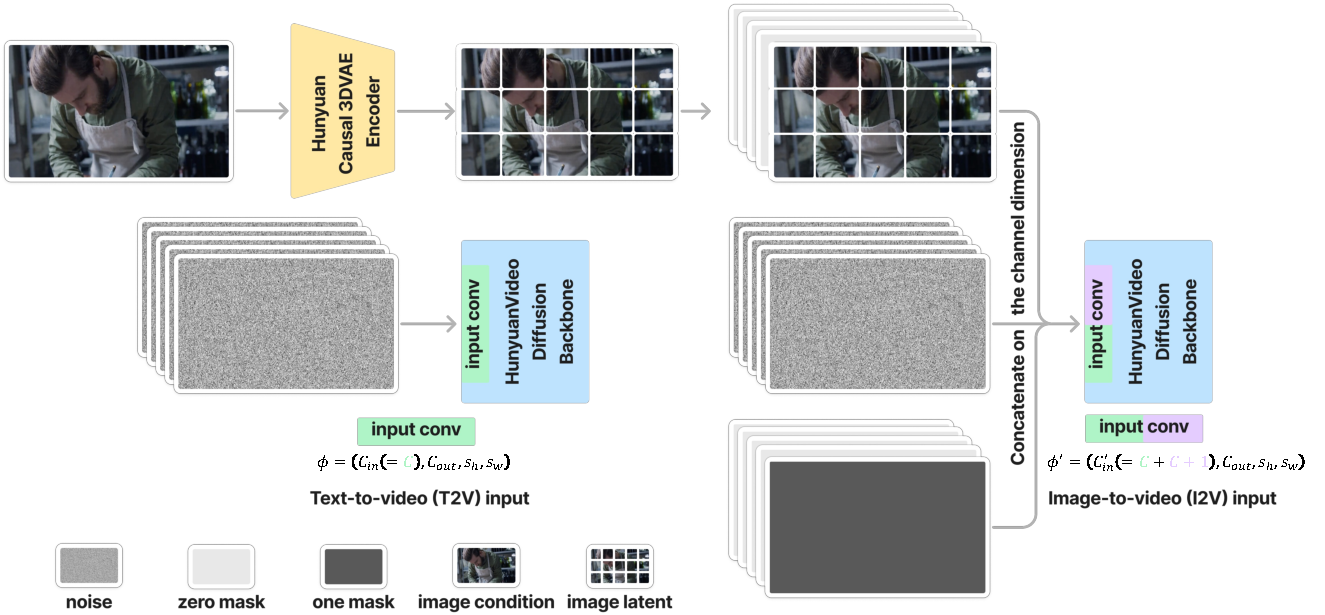
\includegraphics[width=0.9\linewidth]{figures/I2V.pdf}
    \caption{Differences between text-to-video (T2V) model and image-to-video (I2V) model.}
    \label{fig:i2v}
\end{figure}
Image-to-video (I2V) task is a common application in video generation tasks. It usually means that given an image and a caption, the model uses this image as the first frame to generate a video that matches the caption.
Although the naive \nameofmethod{} is a text-to-video (T2V) model, it can be easily extended to an I2V model.
Specifically, as mentioned in Sec. \ref{sec:architecture}, the T2V model's input is a latent $X$ with a shape of $T \times C \times H \times W$, where $T$, $C$, $H$ and $W$ represent the frame, channel, height and width of the compressed video respectively.
Similar to Emu \cite{girdhar2023emu}, in order to introduce image condition $I$, we treat $I$ as the first frame of a video and apply zero-padding to create a $T \times C \times H \times W$ tensor $I_o$, as shown in Fig. \ref{fig:i2v}.
Additionally, we employ a binary mask $m$ with dimensions $T \times 1 \times H \times W$, where the first temporal position is set to 1, and all other positions are set to zero. Then the latent $X$, the tensor $I_o$ and the mask $m$ are concatenated along the channel dimension to form the input for the model.
Note that since the channel of the input tensor has changed from $C$ to $2C+1$, as shown in Fig. \ref{fig:i2v}, we need to adjust the parameters of the first convolutional module of the model from $\phi=(C_{in}(=C), C_{out}, s_h, s_w)$ to $\phi^{\prime}=(C_{in}^{\prime}(=2C+1), C_{out}, s_h, s_w)$, where each component corresponds to the input channel $C_{in}/C_{in}^{\prime}$, output channel $C_{out}$, height of the convolutional kernel $s_h$, and width of the convolutional kernel $s_w$.
In order to retain the representation ability of the T2V model, the first $C$ input channels of $\phi^{\prime}$ are directly copied to $\phi$, and the rest are initialized to zero. We pre-train the I2V model on the same data as T2V model, and the results are shown in Fig. \ref{fig:i2v_result}.
\begin{figure}[t]
    \centering
    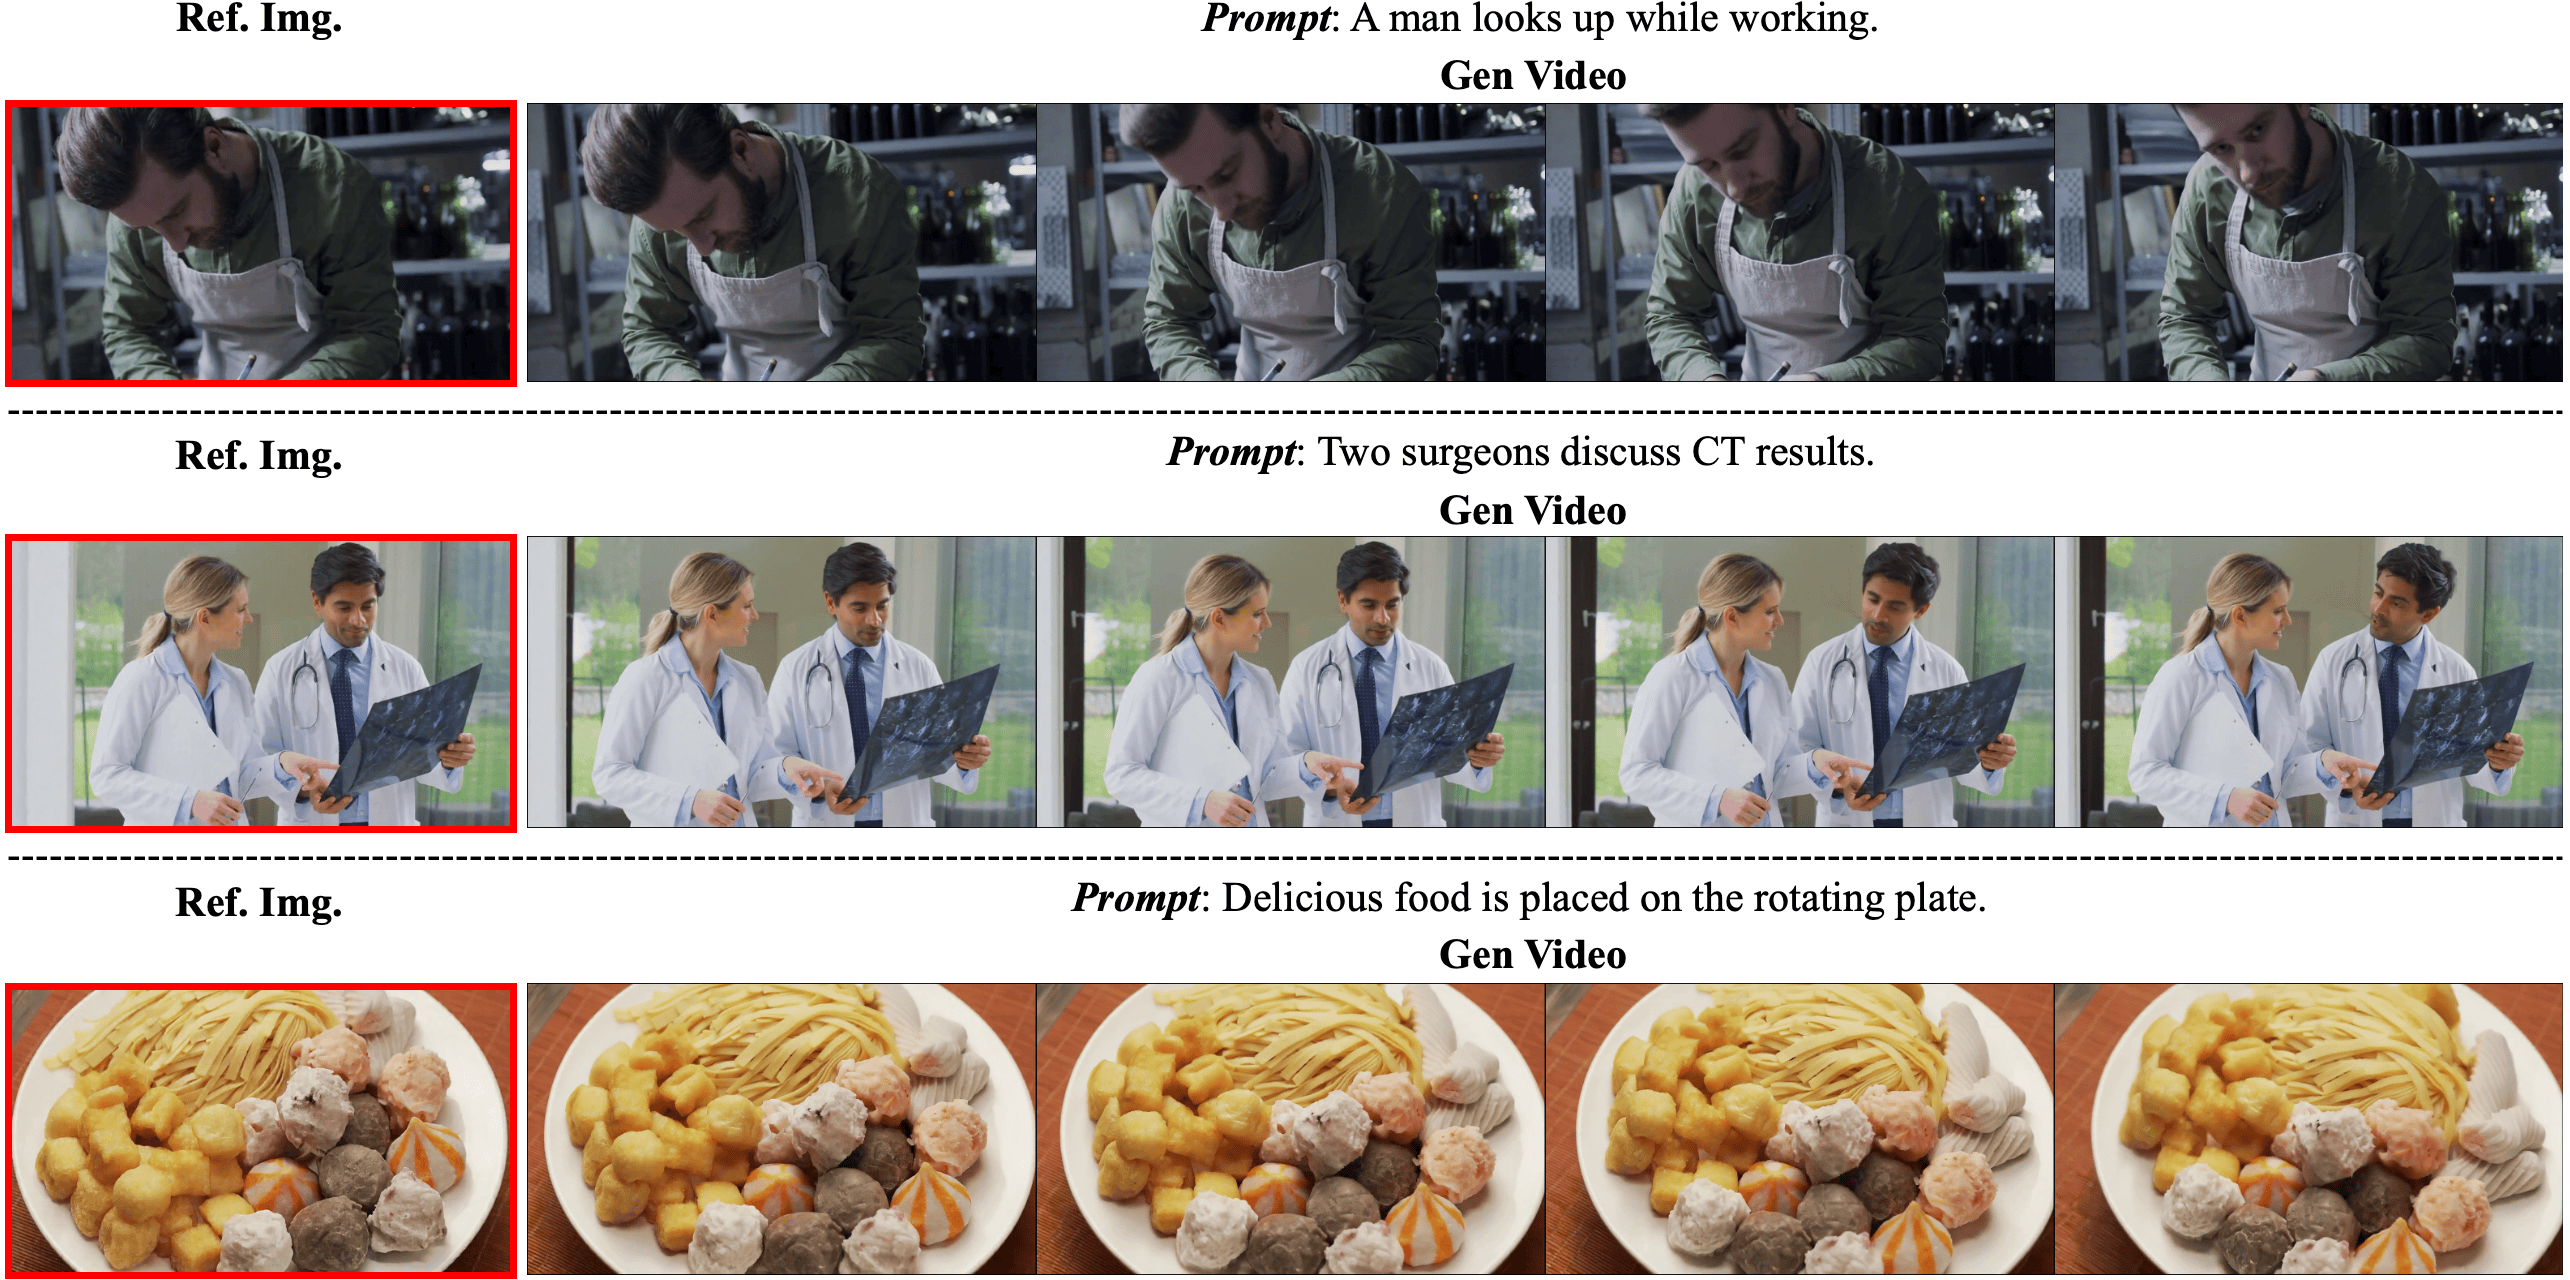
\includegraphics[width=1\linewidth]{figures/i2v_pretraining_result.png}
    \caption{Sample results of the I2V pre-training model.}
    \label{fig:i2v_result}
\end{figure}


\subsubsection{Downstream Task Fine-tuning: Portrait Image-to-Video Generation}
We perform supervised finetuning of our I2V model on two million portrait videos to enhance human's motion and overall aesthetics. In addition to the standard data filtering pipeline described in section \ref{sec:data}, we also apply face and body detectors to filter out the training videos which have more than five persons. We also remove the videos in which the main subjects are small. Finally, the rest videos will be manually inspected to obtain the final high-quality portrait training dataset.

Regarding training, we adopt a progressive fine-tuning strategy, gradually unfreezing the model parameters of the respective layers while keeping the rest frozen during finetuning. This approach allows the model to achieves high performance in the portrait domain without compromising much of its inherent generalization ability, guaranteeing commendable performance in natural landscapes, animals, and plants domains. Moreover, our model also supports video interpolation by using the first and last frames as conditions. We randomly drop the text conditions at certain probability during training to enhance the model's performance. Some demo results are shown in Fig. \ref{fig:portrait_i2v}.

\begin{figure}[h]
    \centering
    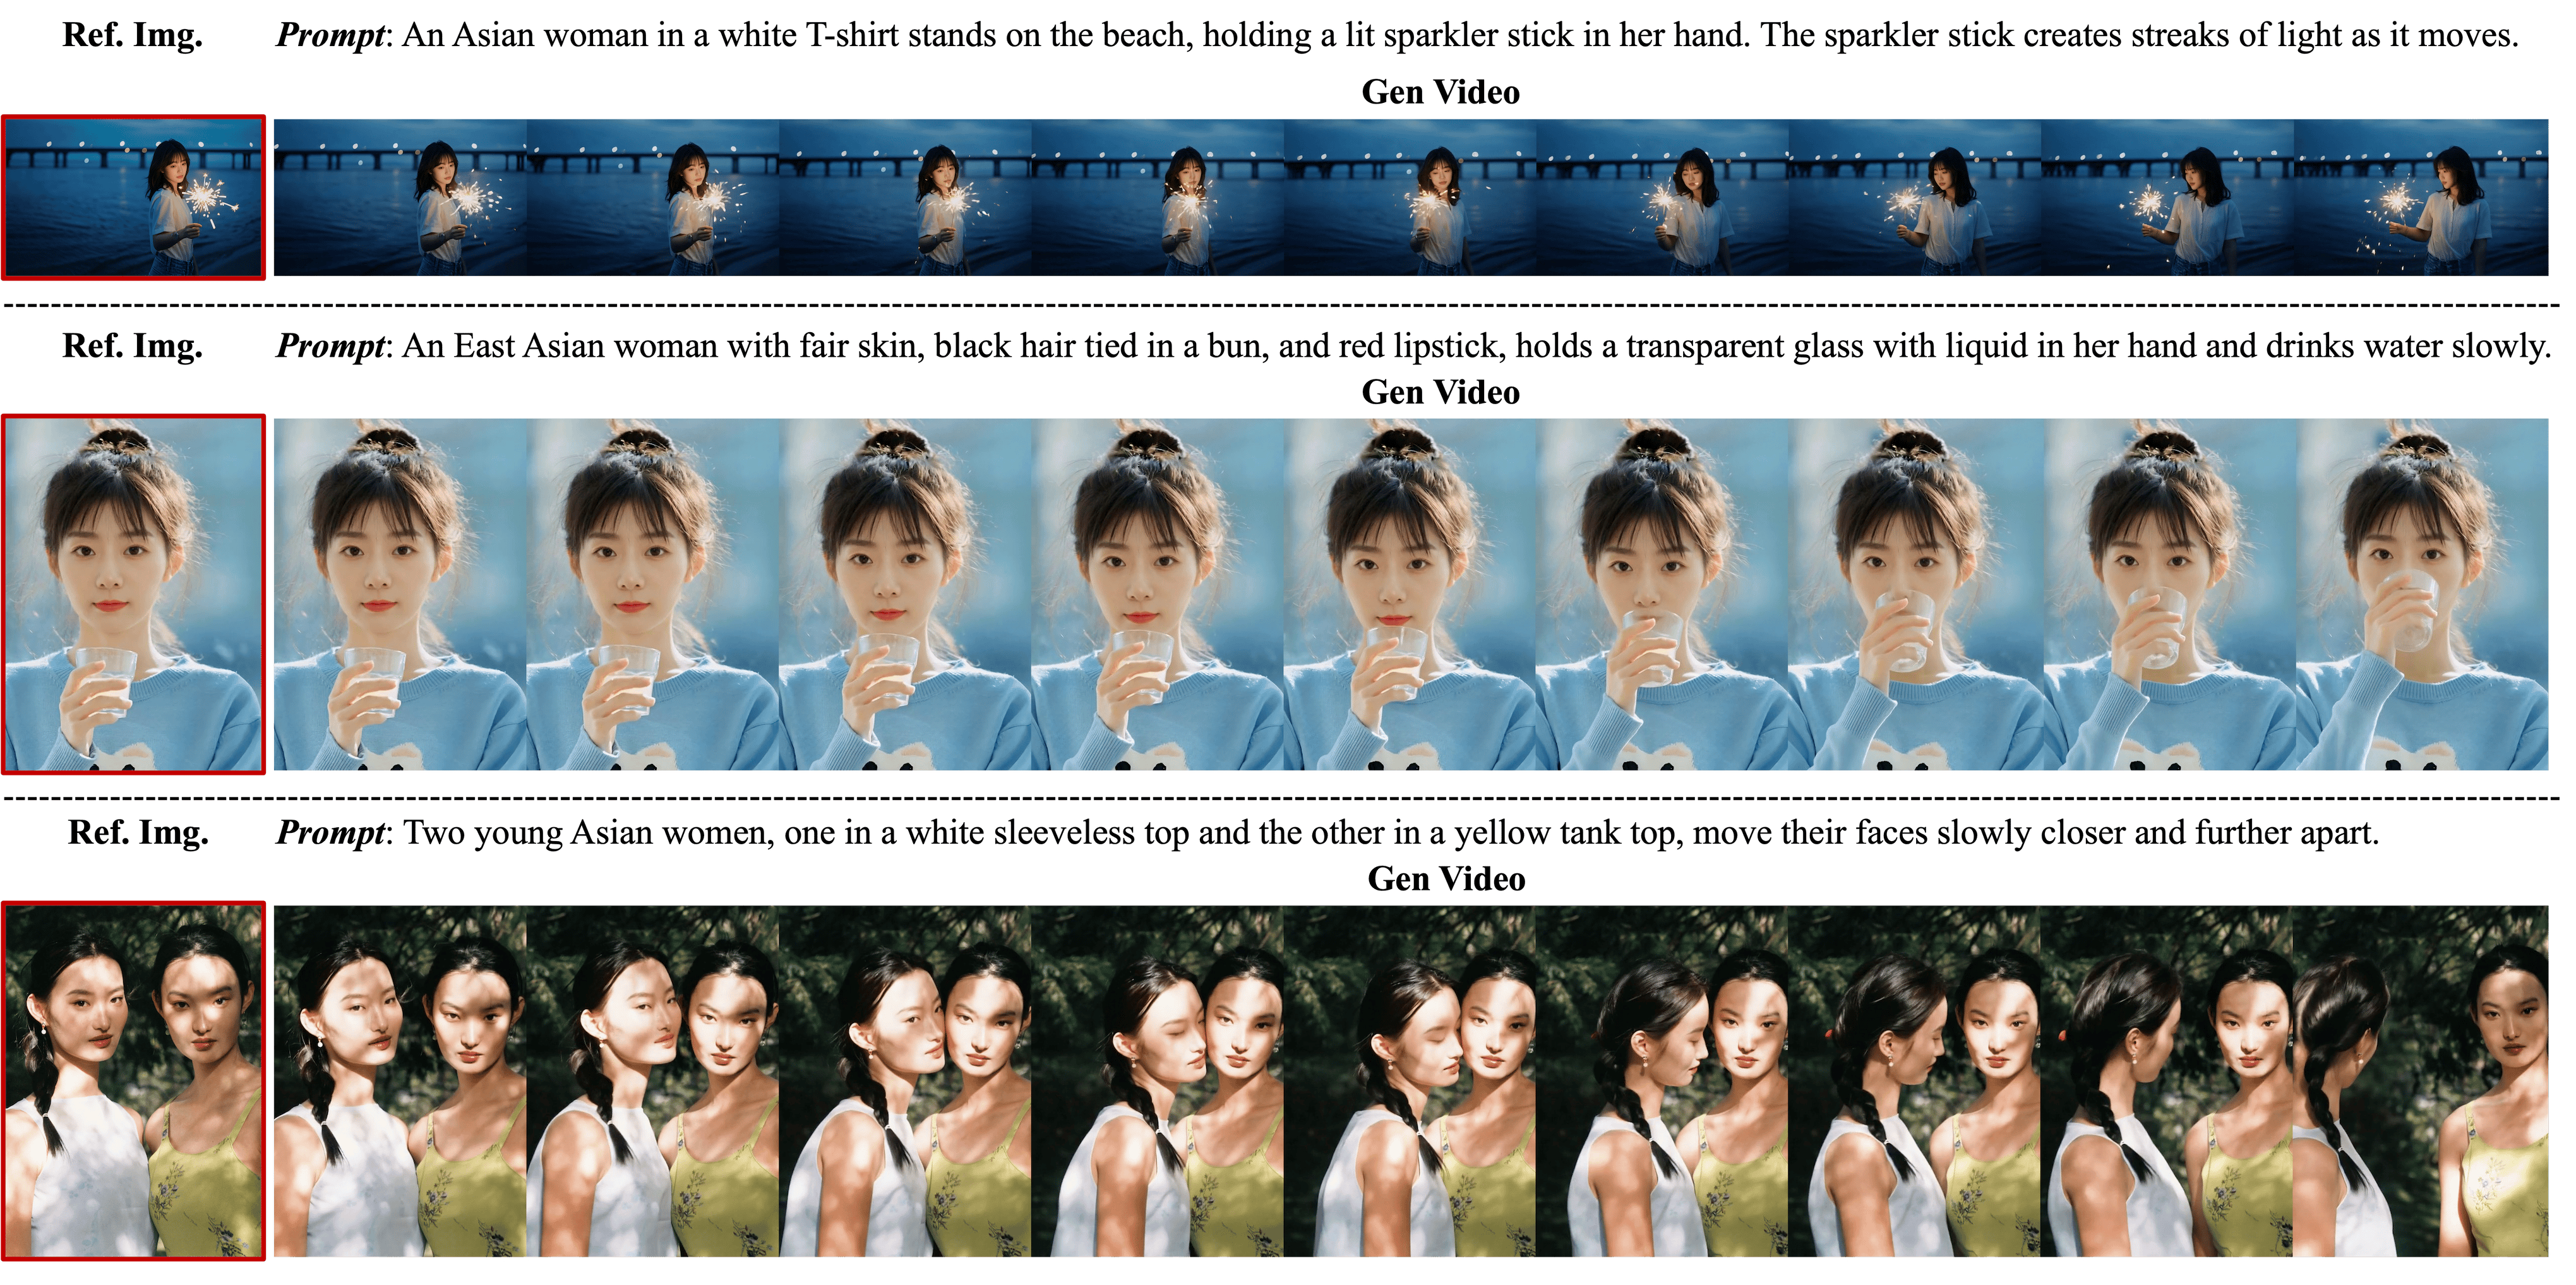
\includegraphics[width=\linewidth]{applications//app_figures/portrait_to_video_new.png}
    \caption{Sample results of our portrait I2V model.}
    \label{fig:portrait_i2v}
\end{figure}

\subsection{Avatar animation}
% \dq{Application Center}

{\nameofmethod} empowers controllable avatar animation in various aspects. It enables animating characters using explicit driving signals(e.g., speech signals, expression templates, and pose templates). In addition, it also integrates the implicit driving paradigm using text prompts. Fig. \ref{fig:application-method} shows how we leverage the power of {\nameofmethod} to animate characters from multi-modal conditions. To maintain strict appearance consistency, we modify the {\nameofmethod} architecture by inserting latent of reference image as strong guidance. As shown in Fig. \ref{fig:application-method} (b, c), we encode reference image using 3DVAE obaining $z_{\rm ref} \in \mathbb{R}^{1 \times c \times h \times w}$, where $c = 16$. Then we repeat it $t$ times along temporal dimension and concatenate with $z_t$ in channel dimension to get the modified noise input $\hat{z}_t \in \mathbb{R}^{t \times 2c \times h \times w}$. To achieve controllable animation, various adapters are employed. We describe them in following.

\begin{figure}[h]
    \centering
    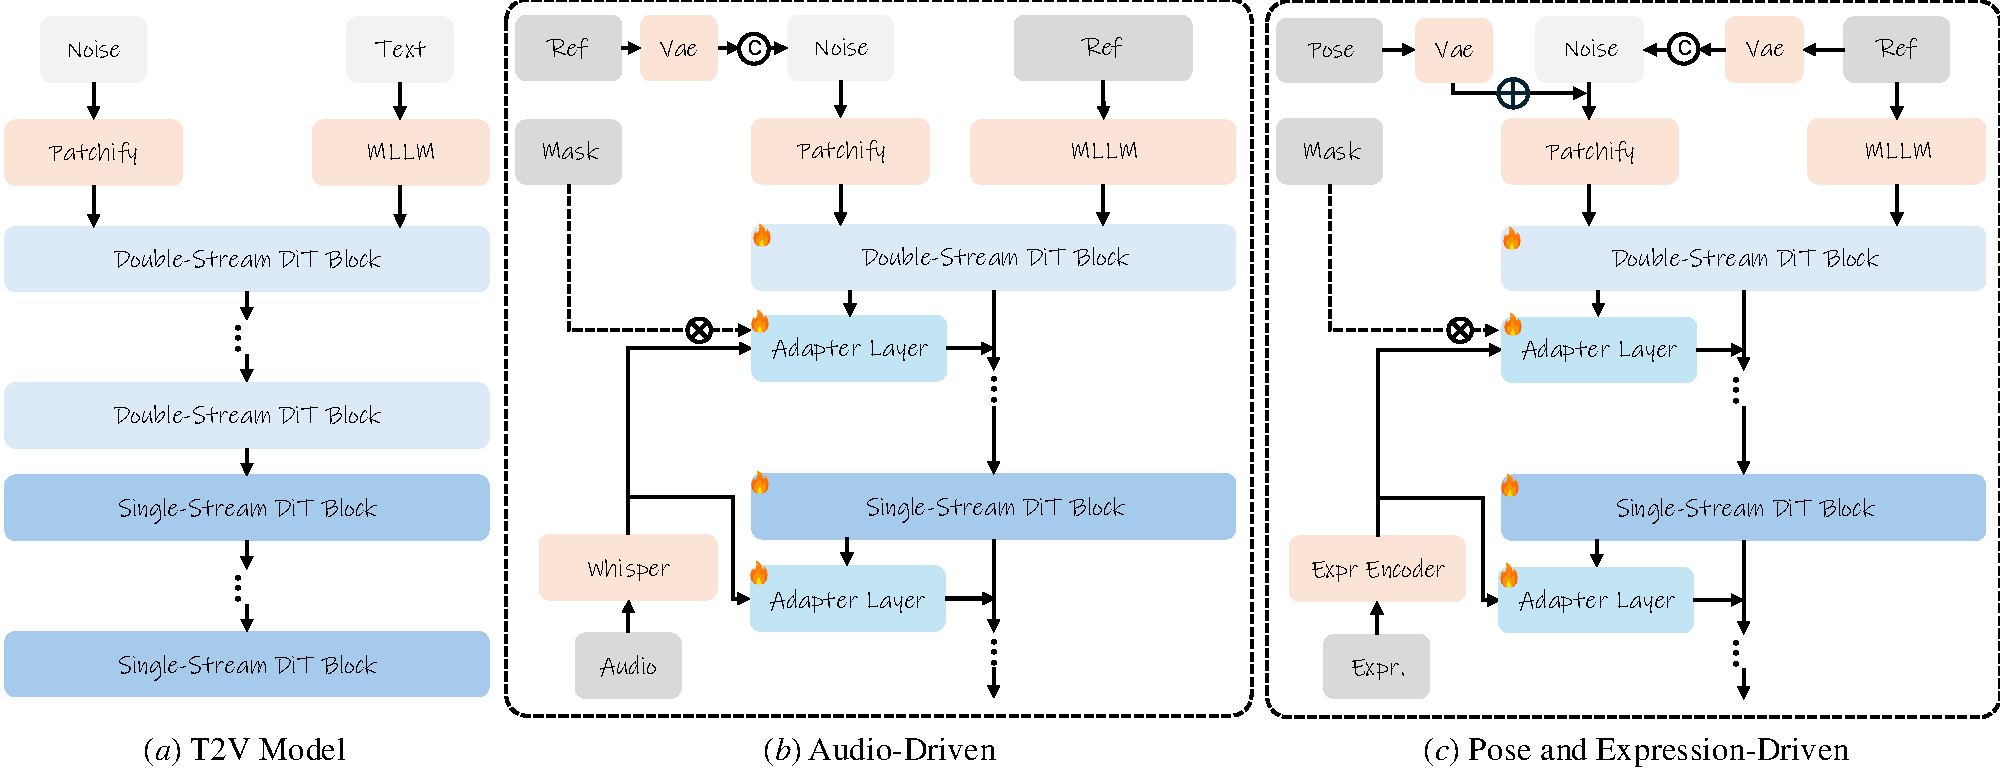
\includegraphics[width=\linewidth]{applications/app_figures/method.pdf}
    \caption{\textbf{Overview of Avatar Animation built on top of \nameofmethod}. We adopt 3D VAE to encode and inject reference and pose condition, and use additional cross-attention layers to inject audio and expression signals. Masks are employed to explicitly guide where they are affecting.}
    \label{fig:application-method}
\end{figure}

\subsubsection{Upper-Body Talking Avatar Generation}

In recent years, audio-driven digital human algorithms have made significant progress, especially in the performance of the talking head. Early algorithms, such as loopy~\cite{ye2024mimic}, emo~\cite{tian2024emo}, and hallo~\cite{xu2024hallo}, mainly focused on the head area, driving the digital human's facial expressions and lip shapes by analyzing audio signals. Even earlier algorithms, like wav2lip~\cite{prajwal2020lip} and DINet~\cite{zhang2023dinet}, concentrated on modifying the mouth region in the input video to achieve lip shape consistency with the audio. However, these algorithms are usually limited to the head area, neglecting other parts of the body. To achieve a more natural and vivid digital human performance, we propose an audio-driven algorithm extended to the upper body. In this algorithm, the digital human not only synchronizes facial expressions and lip shapes with the audio while speaking but also moves the body rhythmically with the audio.

% \subsubsection{Audio-Driven}
\paragraph{Audio-Driven}
Based on the input audio signal, our model can adaptively predict the digital human's facial expressions and posture action information . This allows the driven character to speak with emotion and expression, enhancing the digital human's expressiveness and realism. 
As shown in  Fig. \ref{fig:application-method} (b), for the single audio signal-driven part, the audio passes through the whisper feature extraction module to obtain audio features, which are then injected into the main network in a cross-attention manner. It should be noted that the injection process will be multiplied by the face-mask to control the audio's effect area. While enhancing the head and shoulder control ability, it will also greatly reduce the probability of body deformation. To obtain more lively head movements, head pose motion parameters and expression motion parameters are introduced and added to the time step in an embedding manner. During training, the head motion parameters are given by the variance of the nose tip keypoint sequence, and the expression parameters are given by the variance of the facial keypoints. 
% During inference, fixed values pose=8 and exp=16 are used for inference.
% However, since there is no strong semantic correlation between audio itself and gestures, for some scenes, single audio-driven may cause the head and shoulder part to move naturally with the audio, but the body part, especially the hands,  tends to move slightly or unnaturally. To solve this problem, we introduce text information.


% \subsubsection{Audio and Text Driven}
% \paragraph{Audio and Text Driven}
% Based on aries' powerful semantic understanding ability, we inject a prompt describing actions as the model's text information. In this way, during video generation, the model can not only use audio signals to drive the digital human's actions but also refer to text information to provide more accurate and natural action information. 

% Unlike audio-driven, when we jointly drive with audio and text, we remove the face-mask, allowing the audio's effect area to be released and enabling the character to have a larger range of motion. Second, we removed the encoding of reference images based on llava. During audio-driven, without text injection, we use reference images for information injection. When there is text information, we prioritize aligning with the model's original input. Additionally, we retain the head pose motion parameters and expression parameters.

% By combining audio and text information, our algorithm can achieve a more natural and lively digital human performance. This method not only improves the realism of the digital human but also enhances its adaptability and expressiveness in different scenarios. 


\begin{figure}
    \centering
    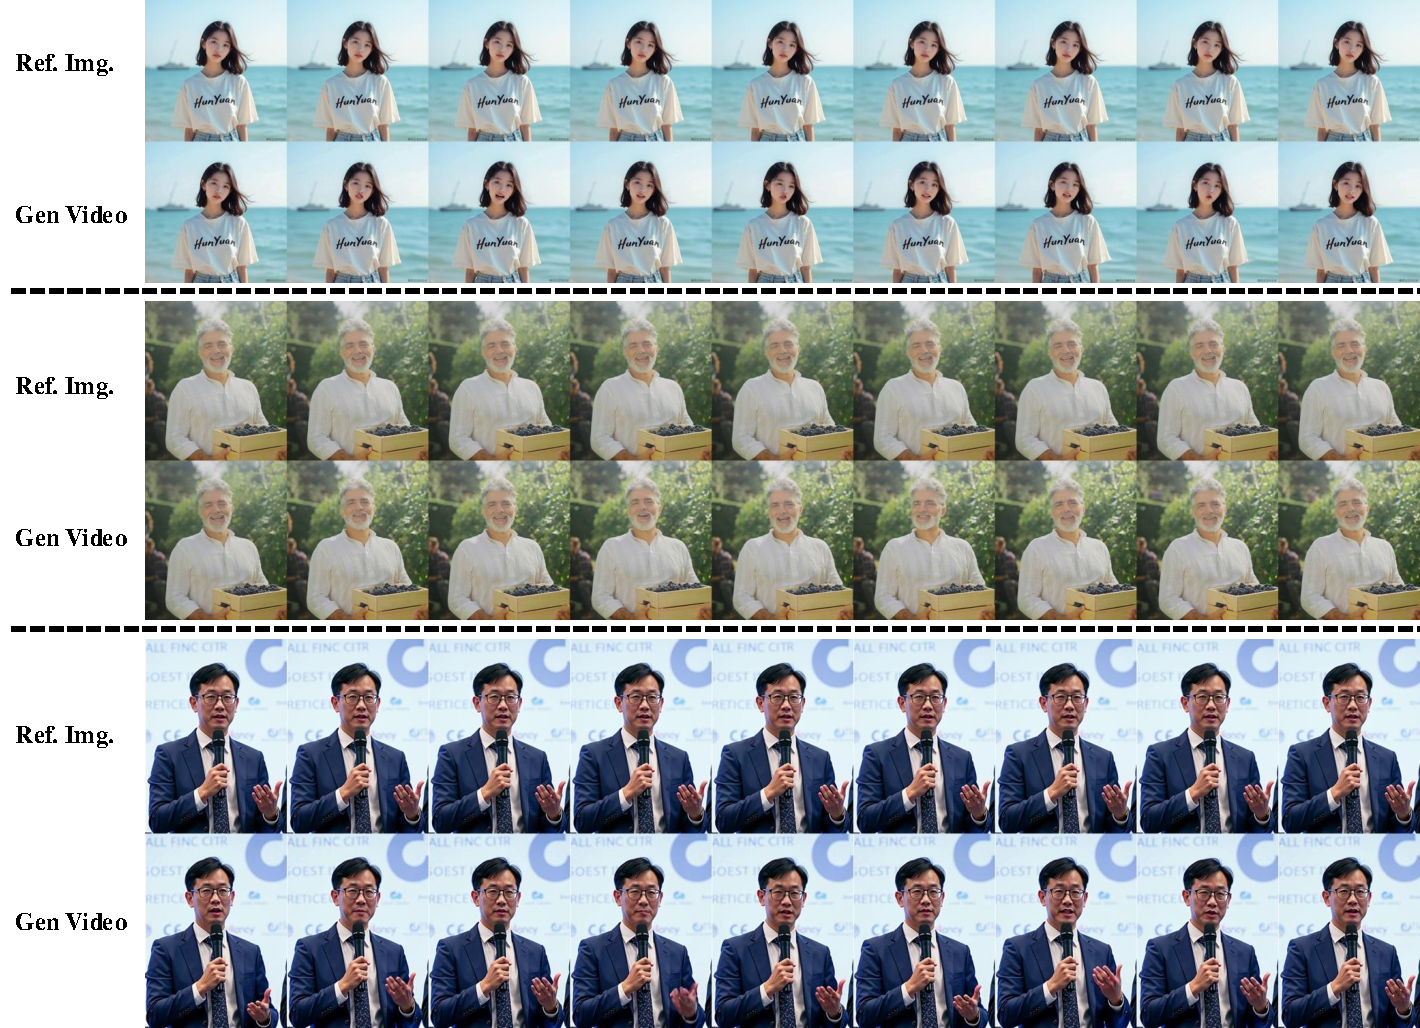
\includegraphics[width=\linewidth]{applications/app_figures/audio-1.pdf}
    \caption{\textbf{Audio-Driven}. {\nameofmethod} can generate vivid talking avatar videos.}
    \label{fig:application-audio}
\end{figure}

\begin{figure}
    \centering
    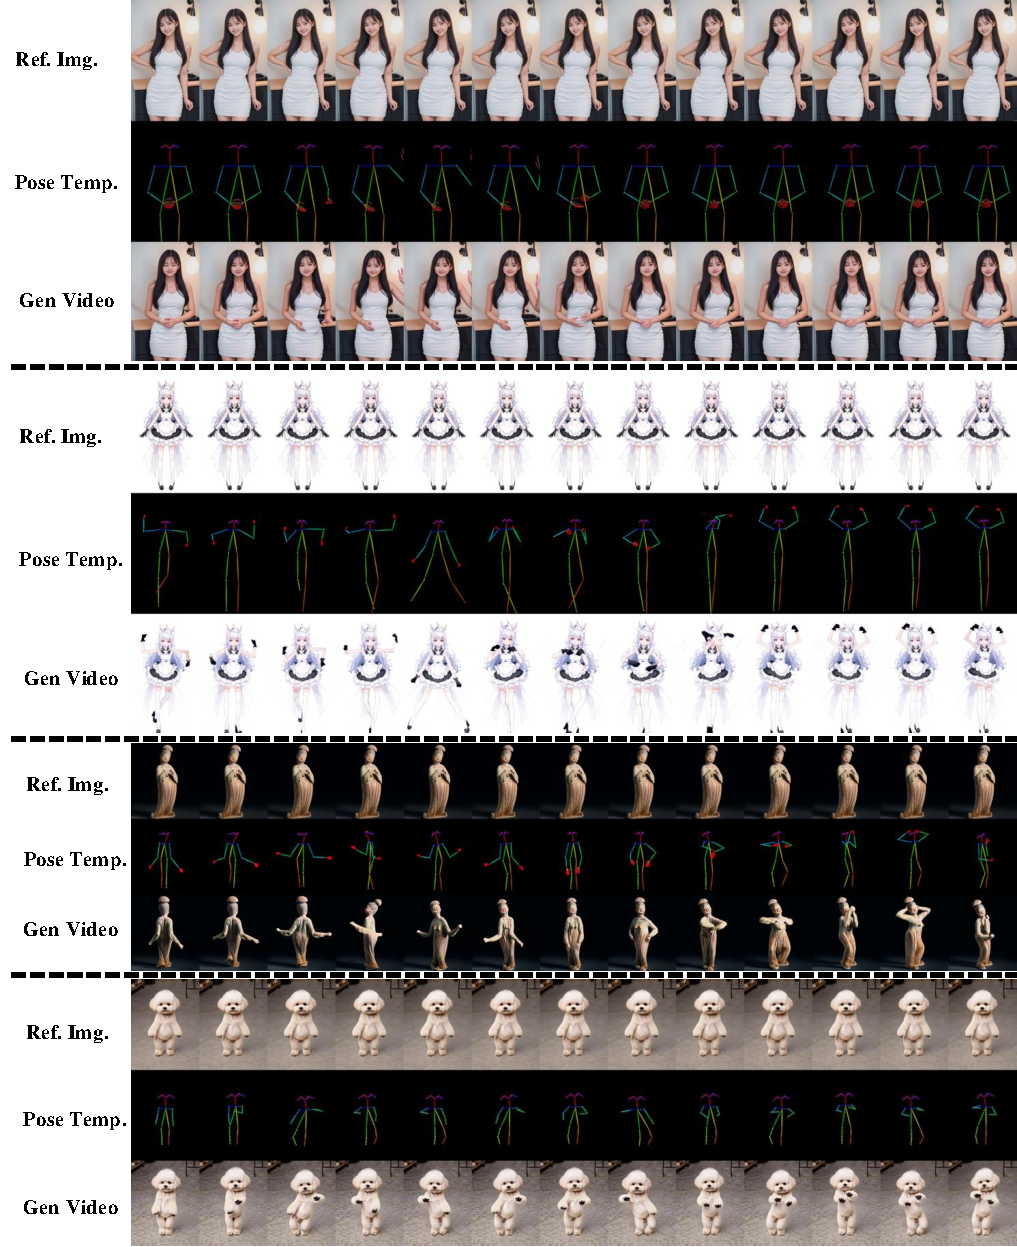
\includegraphics[width=\linewidth]{applications/app_figures/pose.pdf}
    \caption{\textbf{Pose-Driven}. {\nameofmethod} can animate wide variety of characters with high quality and appearance consistency under various poses.}
    \label{fig:application-pose}
\end{figure}


\begin{figure}
    \centering
    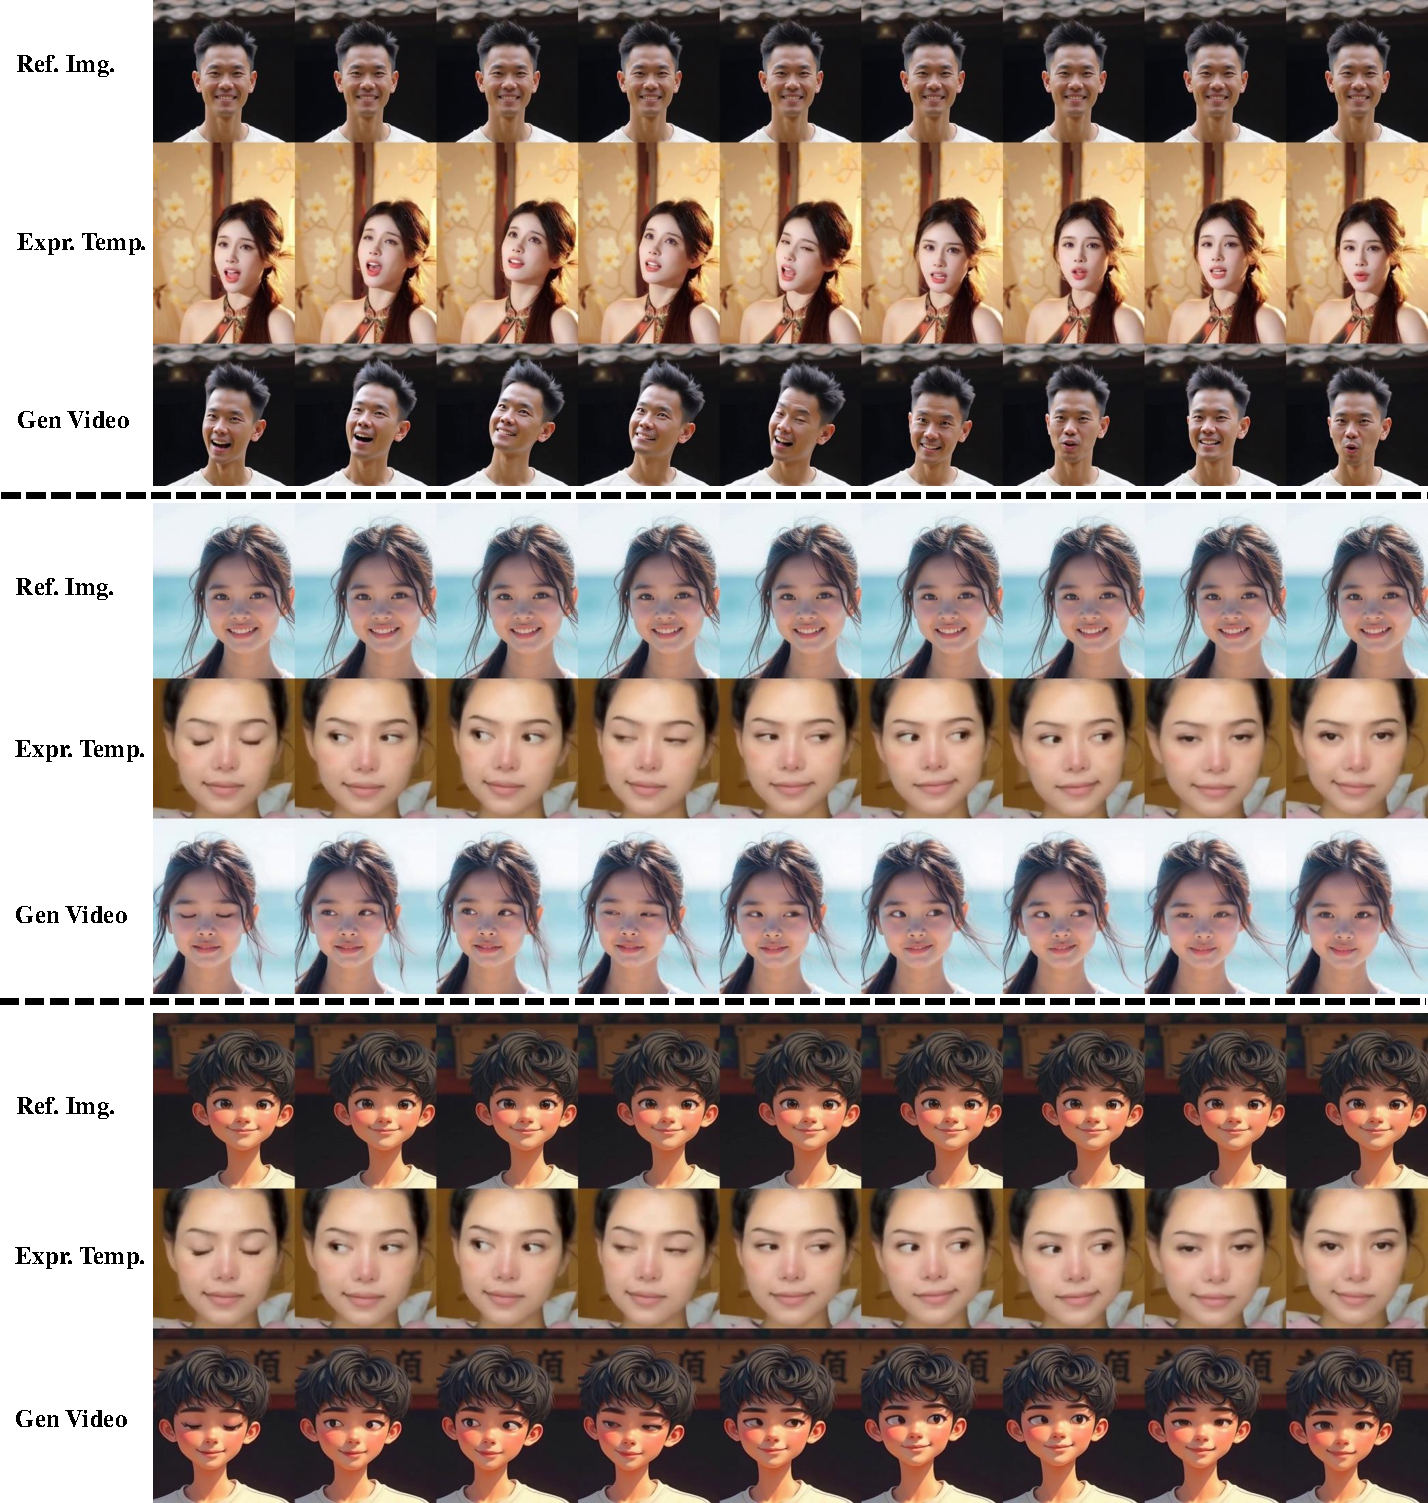
\includegraphics[width=\linewidth]{applications/app_figures/expr-1.pdf}
    \caption{\textbf{Expression-Driven}. {\nameofmethod} can accurately control facial movements of wide-variety of avatar styles.}
    \label{fig:application-expr}
\end{figure}

\begin{figure}[h]
    \centering
    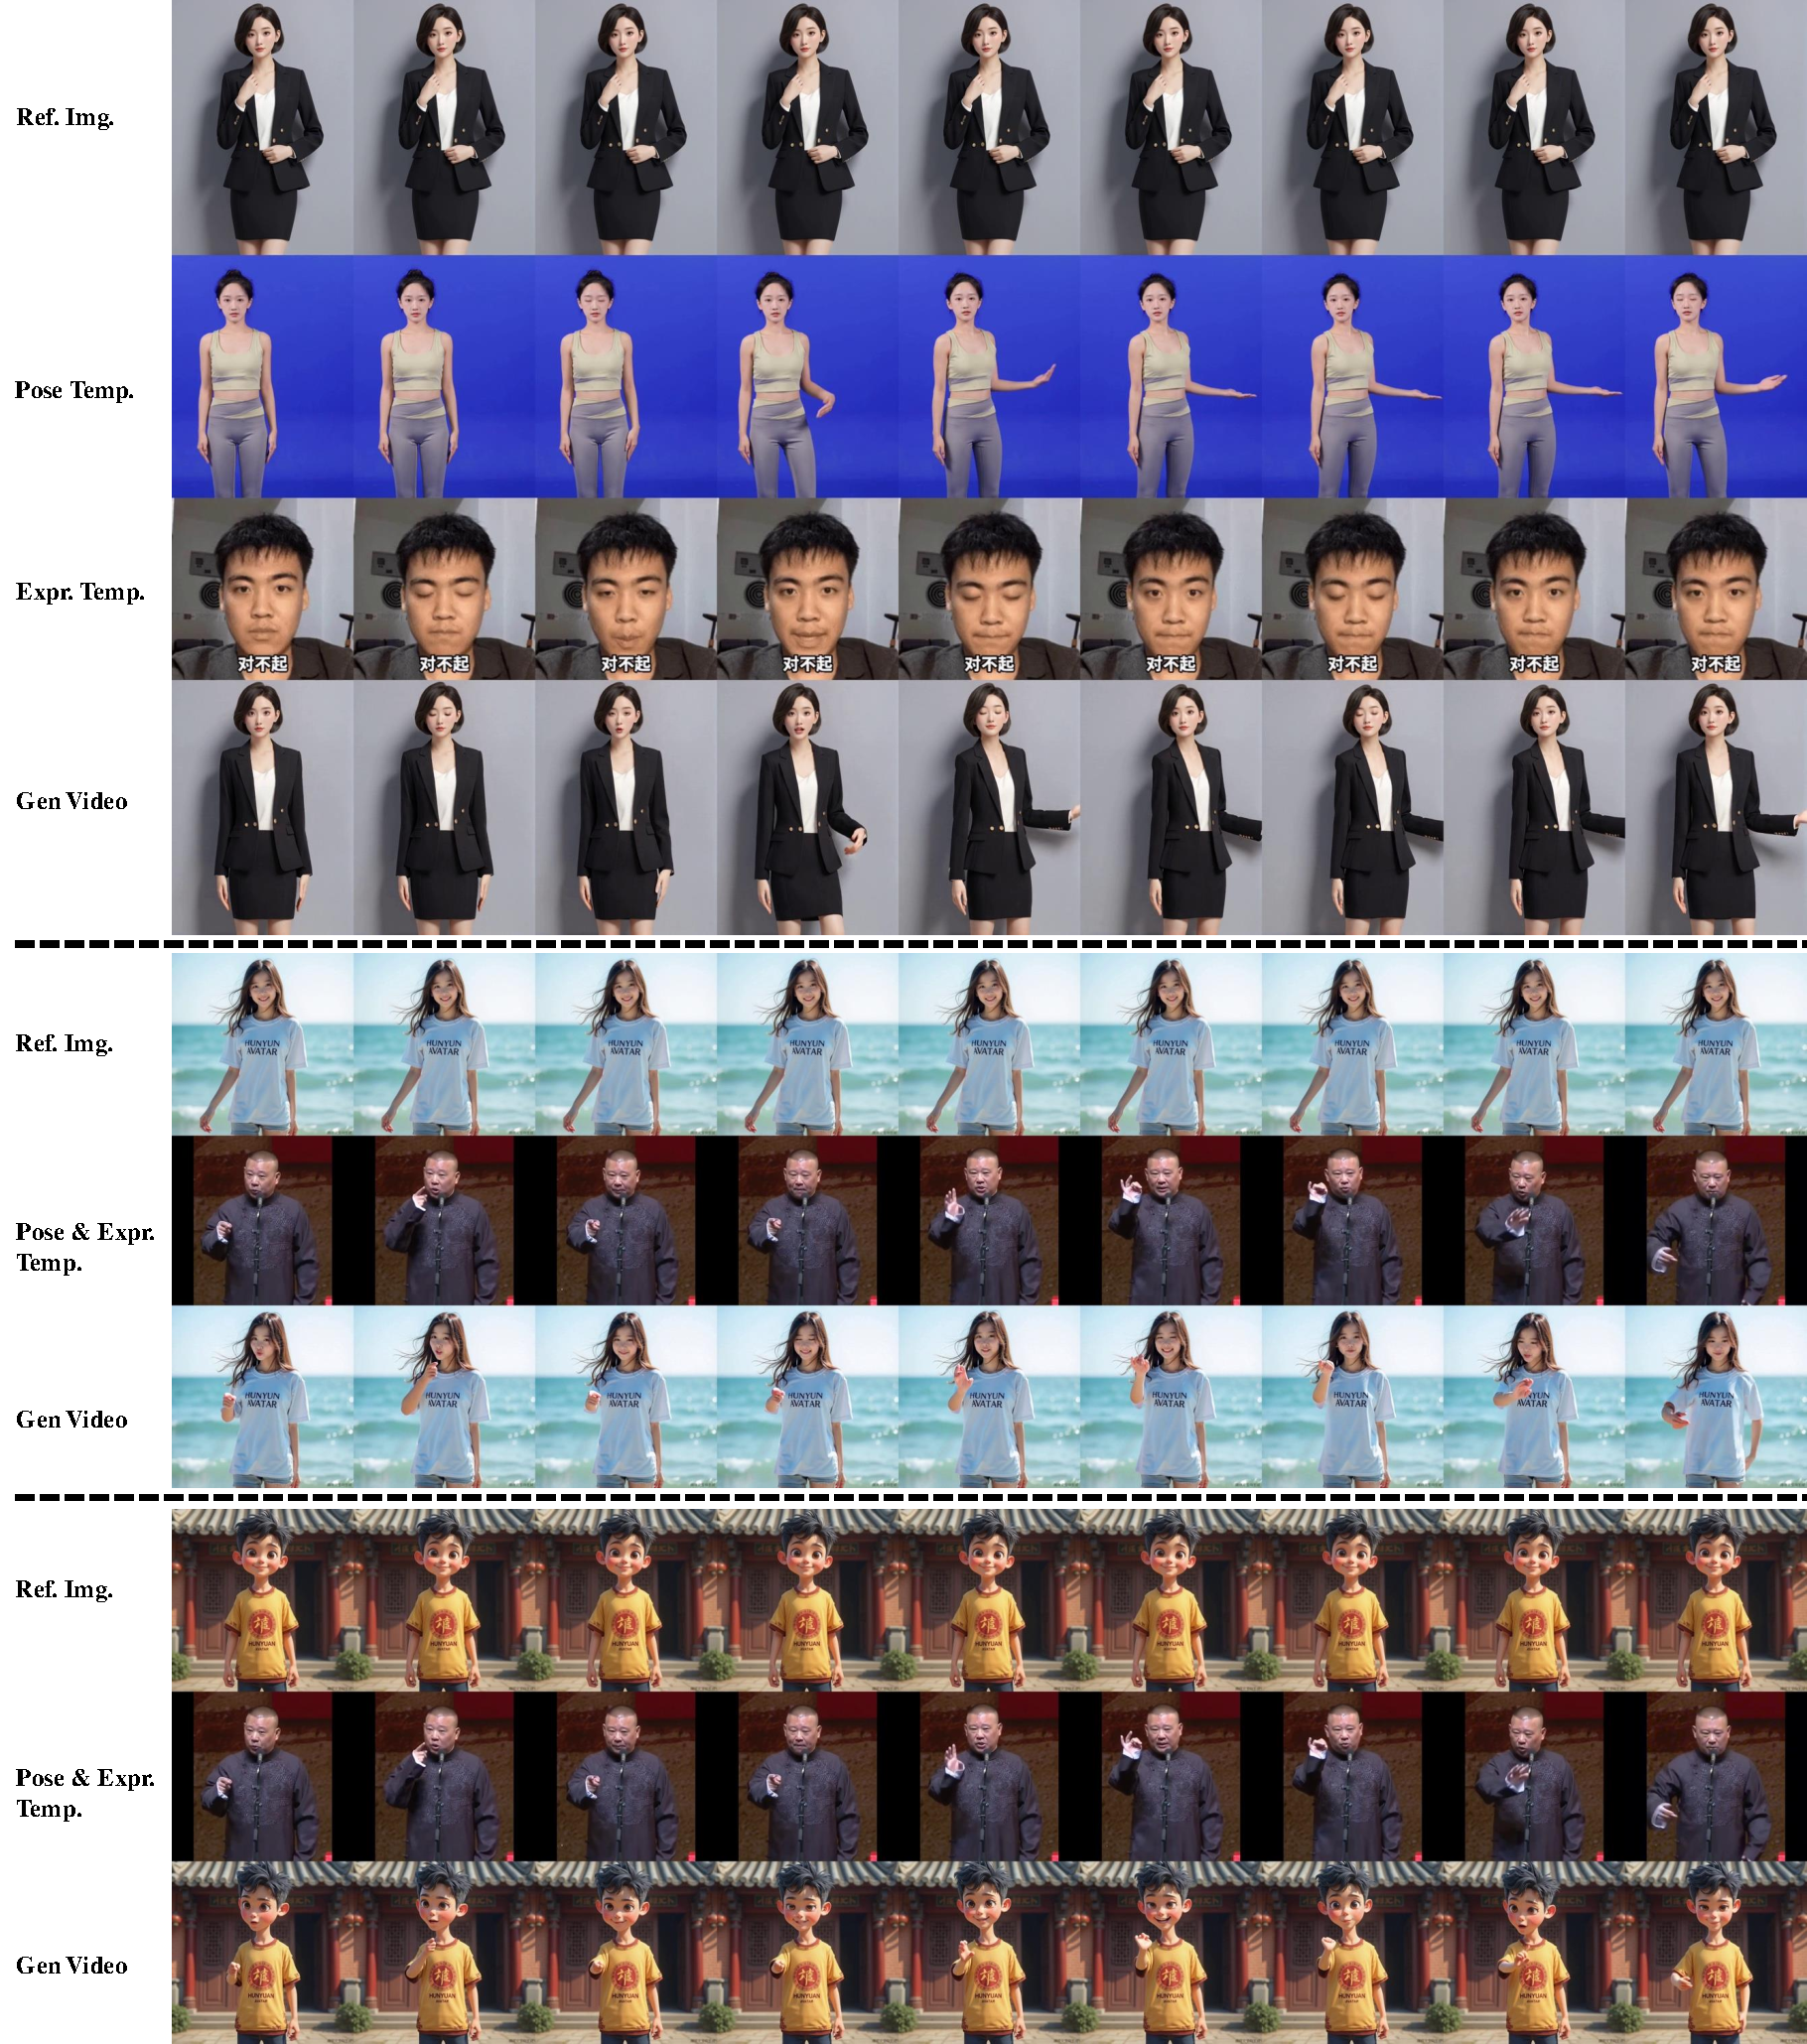
\includegraphics[width=\linewidth]{applications/app_figures/pose-expr-1.pdf}
    \caption{\textbf{Hybrid Condition-Driven}. {\nameofmethod} supports full control with multiple driving sources across various avatar characters.}
    \label{fig:application-pose-expr}
\end{figure}

\subsubsection{Fully-Controlled Whole-Body Avatar Generation} Controlling digital character's motion and expression explicitly has been a long-standing problem in both academia and industry, and recent advancement of diffusion models paved the first step to realistic avatar animation. However, current avatar animation solutions suffer from partial controllability due to limited capability of foundation video generation model. We demonstrate that a stronger T2V model boosts the avatar video generation to fully-controllable stage. We show how {\nameofmethod} serves as strong foundation with limited modifications to extent general T2V model to fully-controllable avatar generation model in Fig. \ref{fig:application-method} (c).

% \subsubsection{Pose-Driven} 
\paragraph{Pose-Driven}
We can control the digital character's body movements explicitly using pose templates. We use Dwpose~\cite{yang2023effective} to detect skeletal video from any source video, and use 3DVAE to transform it to latent space as $z_{\rm pose}$. We argue that this eases the fine-tuning process because both input and driving videos are in image representation, and are encoded with shared VAE, resulting same latent space. We then inject the driving signals to the model by element-wise add as $\hat{z}_t + z_{\rm pose}$. Note that $\hat{z}_t$ contains the appearance information of reference image. We use full-parameters finetune with pretrained T2V weights as initialization. 

% \subsubsection{Expression-Driven} 
\paragraph{Expression-Driven}
We can also control the facial expressions of digital character using implicit expression representations. Although facial landmarks are widely adopted in this area~\cite{ma2024follow, chen2024echomimic}, we argue using landmarks brings ID leak due to cross-ID misalignment. Instead, we use implicit representations as driving signals for their ID and expression disentanglement capabilities. In this work, we use VASA~\cite{xu2024vasa} as expression extractor. As shown in Fig. \ref{fig:application-method} (c), we adopt a light-weight expression encoder to transform the expression representation to token sequence in latent space as $z_{\rm exp} \in \mathbb{R}^{t \times n \times c}$, where $n$ is the number of tokens per frame. Typically, we set $n = 16$. Unlike pose condition, we inject $z_{\rm exp}$ using cross-attention because $\hat{z}_t$ and $z_{\rm exp}$ are not naturally aligned in spatial aspect. We add cross-attention layer ${\rm Attn_{exp}}(q,k,v)$ every $K$ double and single-stream DiT layers to inject expression latent. Denote the hidden states after $i$-th DiT layer as $h_{i}$, the injection of expression $z_{\rm exp}$ to $h_{i}$ could be derived as: $h_{i} + {\rm Attn_{exp}} (h_i, z_{\rm exp}, z_{\rm exp}) \ast \mathcal{M}_{\rm face}$, where $\mathcal{M}_{\rm face}$ is the face region mask that guides where $z_{\rm exp}$ should be applied at, and $\ast$ stands for element-wise multiplication. Also, full-parameters tuning strategy is adopted.


% \subsubsection{Hybrid Condition Driven} 
\paragraph{Hybrid Condition Driven}
Combining both pose and expression driven strategies derives hybrid control approach. In this scenario, the body motion is controlled by explicit skeletal pose sequence, and the facial expression is determined by implicit expression representation. We jointly fine-tune T2V modules and added modules in an end-to-end fasion. During inference, the body motion and facial motion could be controlled by separate driving signals, empowering richer editability. 

% \subsubsection{Application Demos} We present extensive results of avatar animations to show the capability and potential of bringing avatar animation empowered by {\nameofmethod} to next level. We show that {\nameofmethod} serves as a strong foundation model for audio-driven avatar animation, which can synthesize vivid and high-fidelity videos. As shown in Fig. \ref{fig:application-audio}, the generated videos display life-like facial expressions with synchronized lip motions. It also synthesizes videos with rich background dynamics. We also show that {\nameofmethod} boosts the performance of pose-driven animation largely in many aspects, including ability of following complex poses, maintaining details of garment texture and ID consistency along frames (Fig. \ref{fig:application-pose-compare}). In addition, tunning {\nameofmethod} to animate characters shows remarkable ability of generalization. As shown in Fig. \ref{fig:application-pose}, we can animate not only realistic characters, but also non-realistic ones, surprisingly including but not limited to cartoon figures, pottery figurines, anthropomorphic animals, and many others. Fig. \ref{fig:application-expr} shows that finetuning \nameofmethod with added adapter layers synthesize vivid portrait expression videos. It is able to mimic facial motions such as eye gaze, lip motion accurately while maintaining high ID consistency. Lastly, we show that hybrid condition control reveals the potential of fully controllable and editable avatars. As shown in Fig. \ref{fig:application-pose-expr}, we can animate a static avatar character with driving templates from different sources. This hybrid control paradigm paves the route from demo to applications for avatar animation. In addition, we show that hybrid controllability generalizes to both realistic and non-realistic characters (Fig. \ref{fig:application-pose-expr-2}).

% \begin{figure}
%     \centering
%     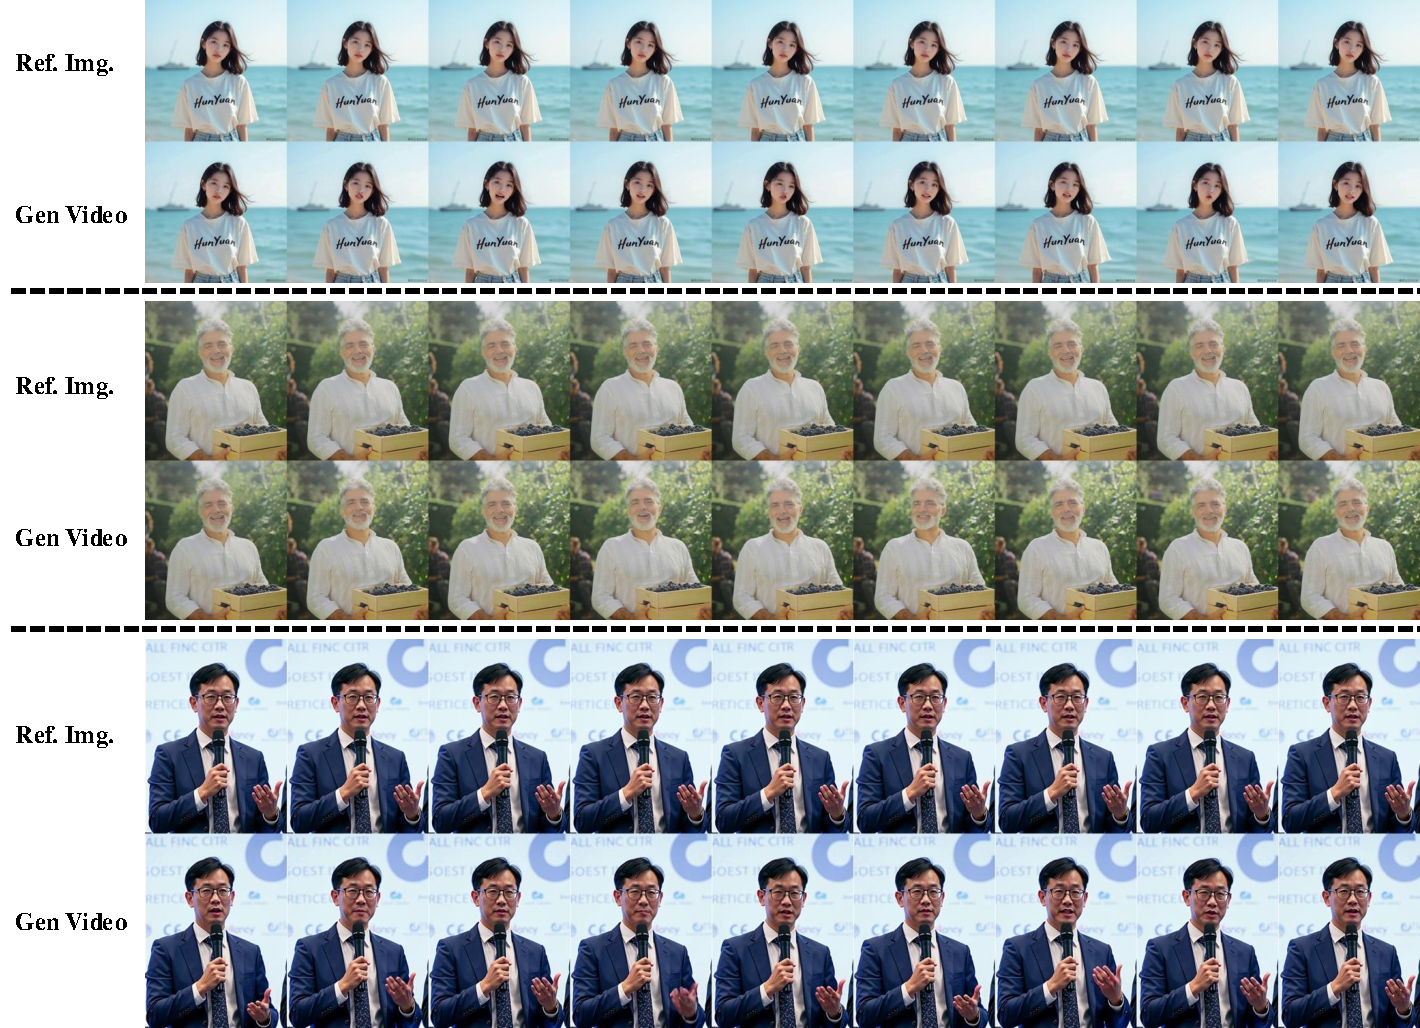
\includegraphics[width=\linewidth]{applications/app_figures/audio-1.pdf}
%     \caption{\textbf{Audio-Driven}. {\nameofmethod} can generate vivid talking avatar videos.}
%     \label{fig:application-audio}
% \end{figure}

% \begin{figure}
%     \centering
%     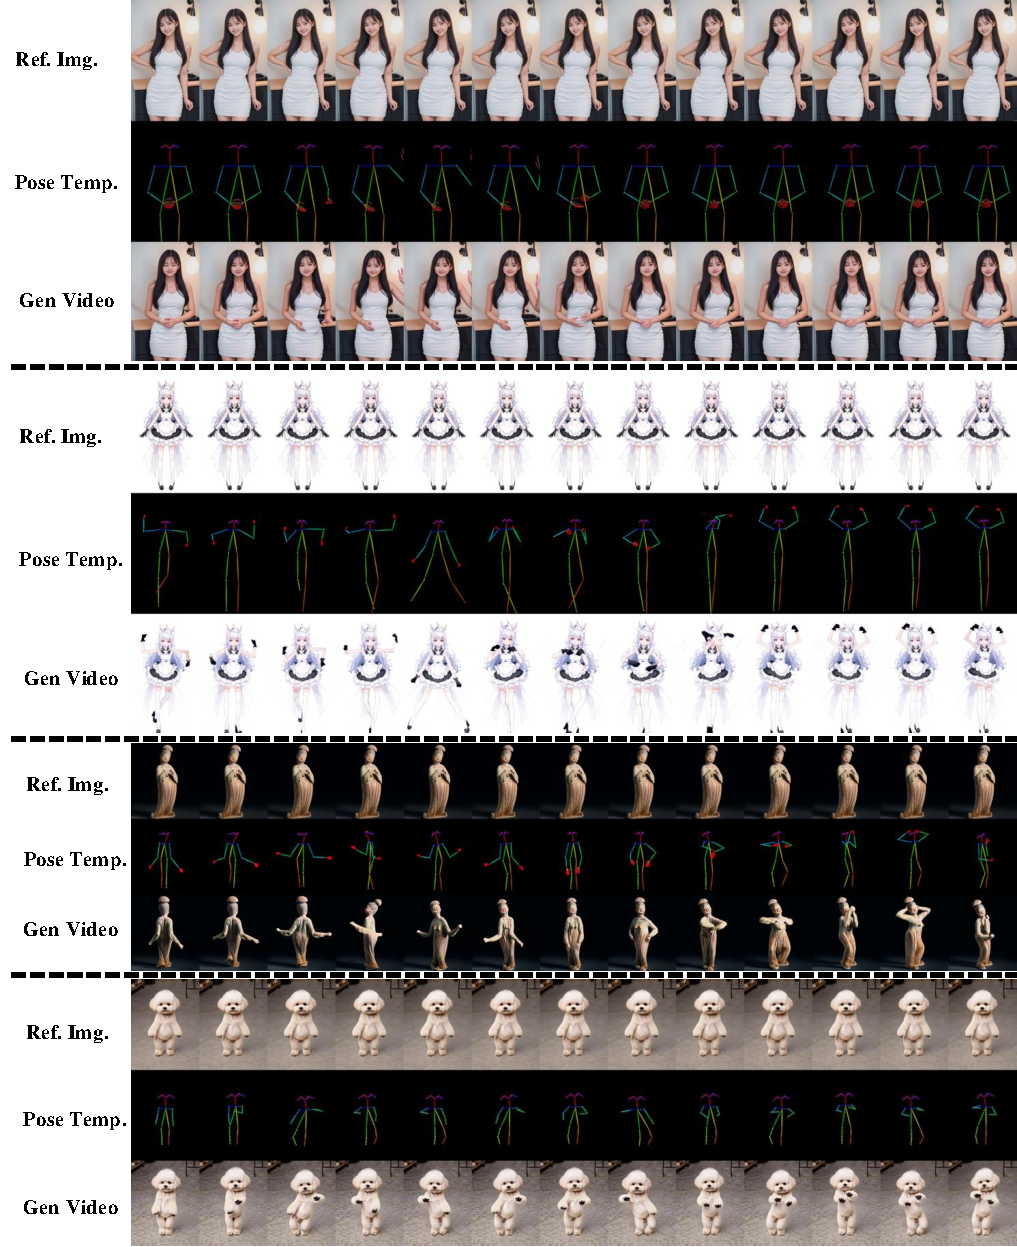
\includegraphics[width=\linewidth]{applications/app_figures/pose.pdf}
%     \caption{\textbf{Pose-Driven}. {\nameofmethod} can animate wide variety of characters with high quality, ID consistency under various poses.}
%     \label{fig:application-pose}
% \end{figure}


% \begin{figure}
%     \centering
%     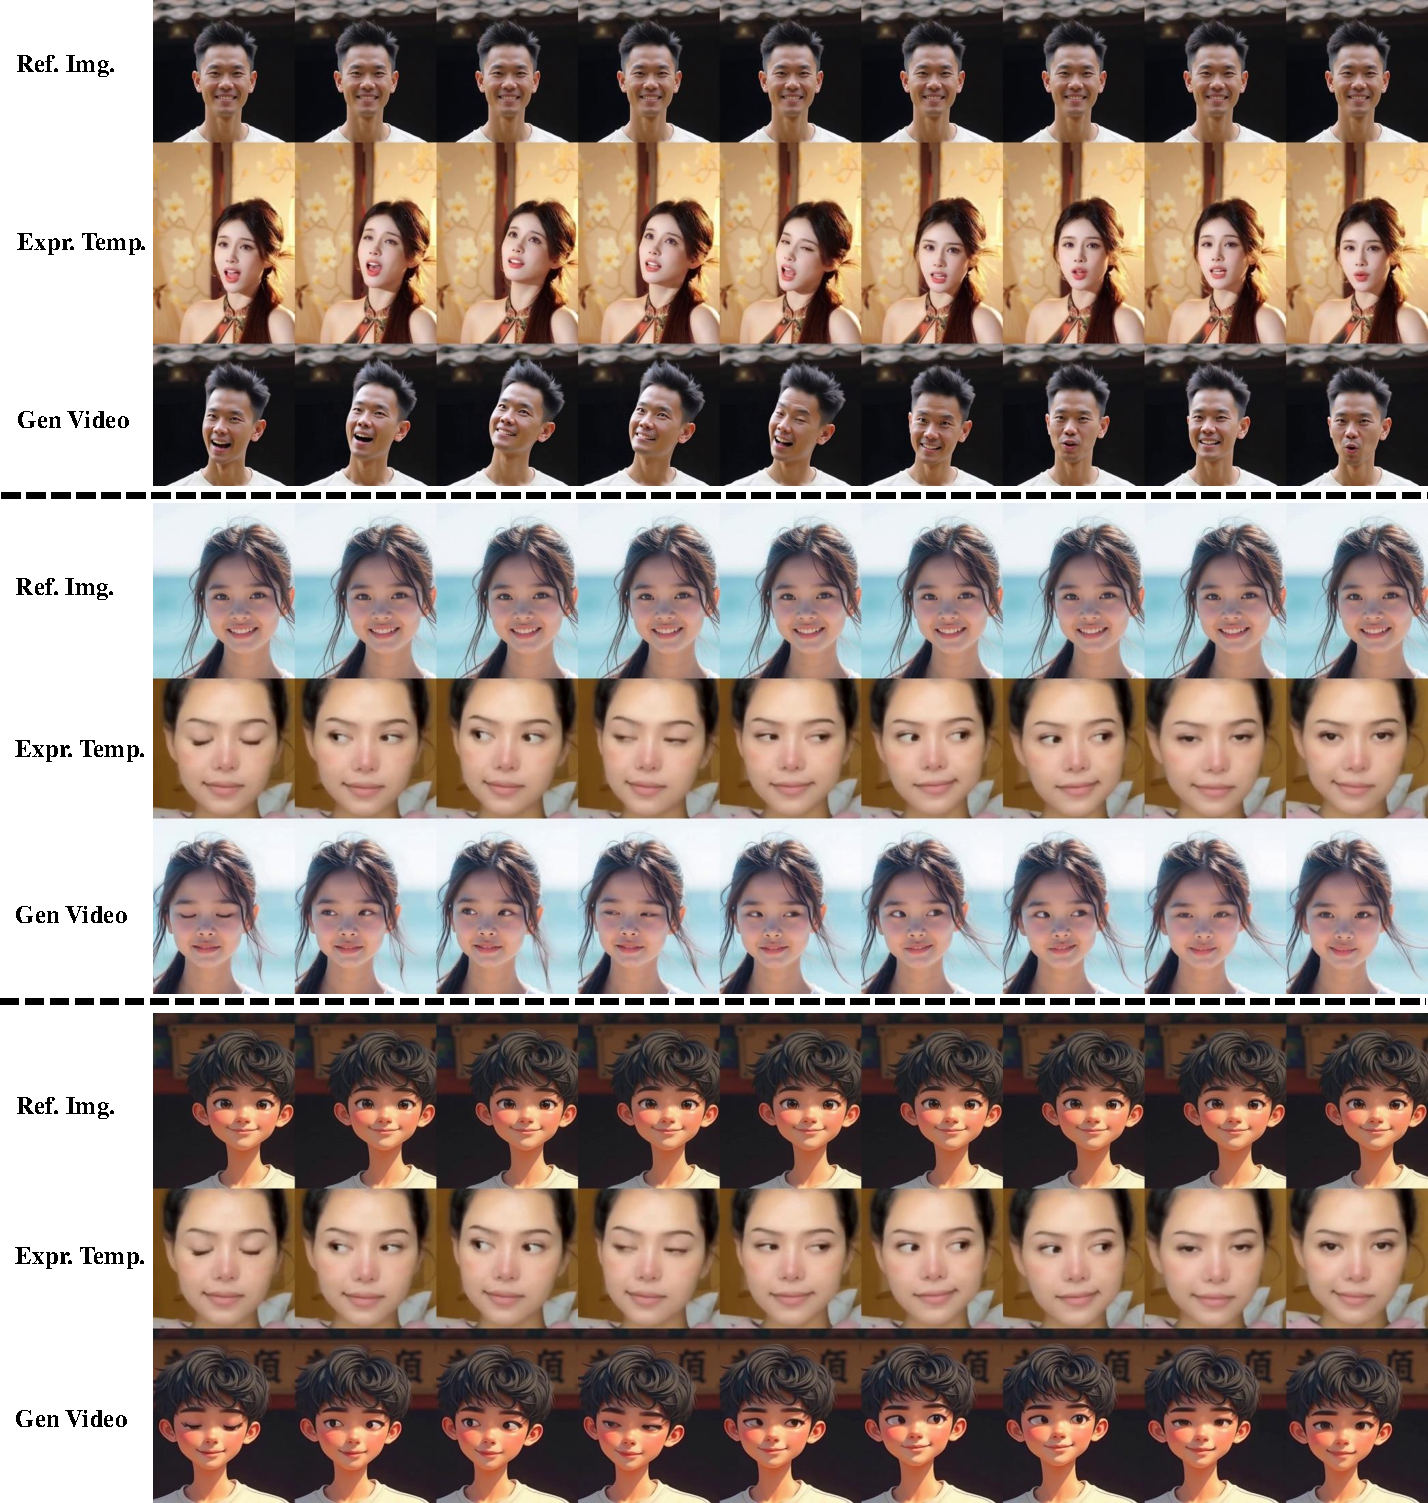
\includegraphics[width=\linewidth]{applications/app_figures/expr-1.pdf}
%     \caption{\textbf{Expression-Driven}. Our method can animate facial expressions of wide-variety of avatar styles.}
%     \label{fig:application-expr}
% \end{figure}

% \begin{figure}[h]
%     \centering
%     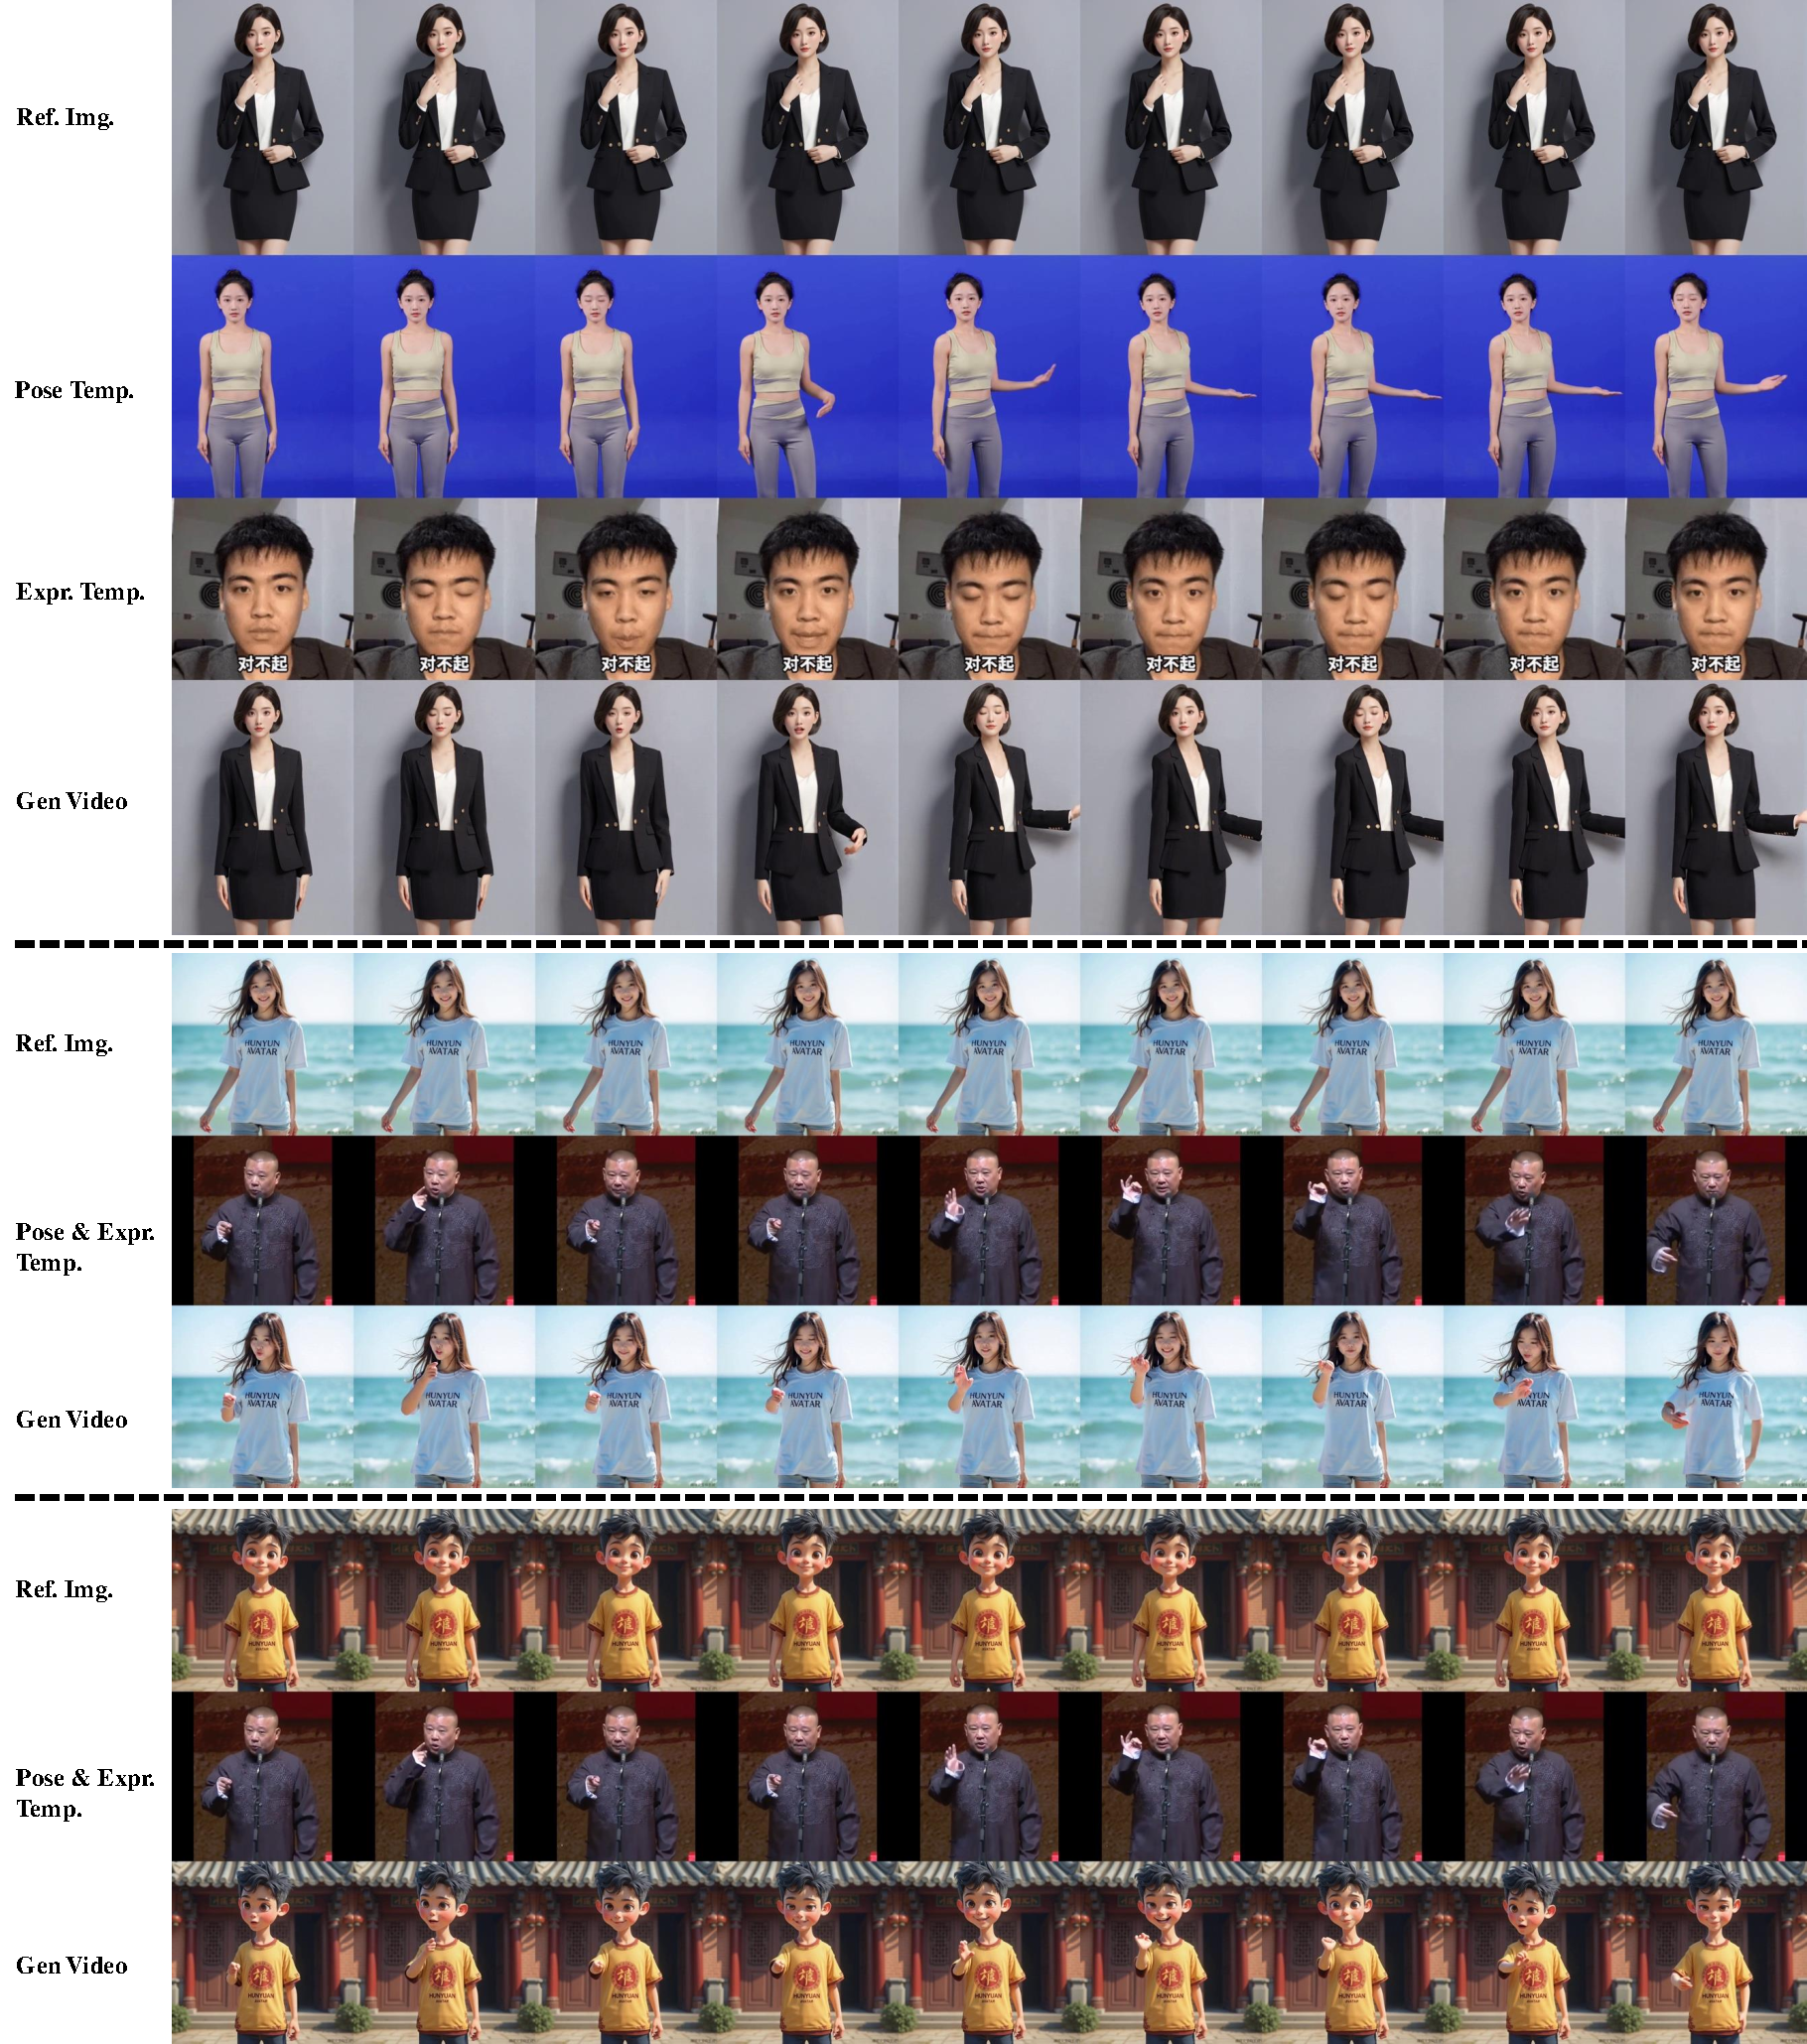
\includegraphics[width=\linewidth]{applications/app_figures/pose-expr-1.pdf}
%     \caption{\textbf{Hybrid Condition-Driven}. Our method supports full control with multiple driving sources across various avatar characters.}
%     \label{fig:application-pose-expr}
% \end{figure}

\subsection{Application Demos} We present extensive results of avatar animations to show the superiority and potential of bringing avatar animation empowered by {\nameofmethod} to next generation.

\paragraph{Audio-Driven}Fig. \ref{fig:application-audio} shows that {\nameofmethod} serves as a strong foundation model for audio-driven avatar animation, which can synthesize vivid and high-fidelity videos. We summarize the superiority of our method in three folds:

\begin{itemize}
    \item \textbf{Upper-body Animation.} Our method can drive not only portrait characters, but also upper-body avatar images, enlarging its range of application scenarios. 
    \item \textbf{Dynamic Scene Modelling.} Our method can generate videos with vivid and realistic background motion, such as the wave undulation, crowd movement, and breeze stirring leaves. 
    \item \textbf{Vivid Avatar Movements.} Our method is able to animate the character talking while gesturing vividly with audio solely.
\end{itemize}

\paragraph{Pose-Driven}We also show that {\nameofmethod} boosts the performance of pose-driven animation largely in many aspects in Fig. \ref{fig:application-pose}:

\begin{itemize}
    \item \textbf{High ID-Consistency.} Our method maintains the ID-consistency well over the frames even with large poses, making it face-swapping free, thereby, could be used as real end-to-end animation solution.
    \item \textbf{Following Complex Poses Accurately.} Our method is able to handle very complex poses such as turning around and hands crossed.
    \item \textbf{High Motion Quality.} Our method has remarkable capability in dynamic modelling. For instance, the results show promising performance in terms of garment dynamics and texture consistency.
    \item \textbf{Generalizability.} Our method presents surprisingly high generalizability. It can animate wide variety of avatar images, such as real human, anime, pottery figurine, and even animals. 
\end{itemize}

\paragraph{Expression-Driven}Fig. \ref{fig:application-expr} presents how {\nameofmethod} enhances the portrait expression animating in three folds:

\begin{itemize}
    \item \textbf{Exaggerated Expression.} Our method is able to animate given portrait to mimic any facial movements even with large poses and exaggerated expressions.
    \item \textbf{Mimicing Eye Gaze Accurately.} We can control the portraits' eye movements acurately given any expression template, even with extreme and large eye balls movements.
    \item \textbf{Generalizability.} Our method has high generalizability. It can animate not only real human portraits, but also anime or CGI characters.
\end{itemize}

\paragraph{Hybrid-Driven} Lastly, we show that hybrid condition control reveals the potential of fully controllable and editable avatars in Fig. \ref{fig:application-pose-expr}. We highlight the superiority as follow:

\begin{itemize}
    \item \textbf{Hybrid Condition Control.} For the first time, our method is able to conduct full control over body and facial motions with siloed or multiple signals, paving the route from demo to applications for avatar animation.
    \item \textbf{Half-body Animation.} Our method supports upper-body full control, enabling rich editability while maintaining high quality and fidelity.
    \item \textbf{Generalizability.} Our method generalize to both real human images and CGI characters. 
\end{itemize}


% \begin{figure}
%     \centering
%     \includegraphics[width=\linewidth]{applications/app_figures/pose-compare.pdf}
%     \caption{\textbf{{\nameofmethod} Boosts Pose-Driven Animation in Many Aspects}. (a) It maintains garment details (sleeves). (b) Better pose following (fingers). (c) Higher ID consistency (faces).}
%     \label{fig:application-pose-compare}
% \end{figure}

% \begin{figure}
%     \centering
%     \includegraphics[width=\linewidth]{applications/app_figures/pose-expr-5.pdf}
%     \caption{\textbf{Animating Wide-Variety of Avatars}. Our method can animate both realistic character (upper pannel) and cartoon style (lower pannel).}
%     \label{fig:application-pose-expr-2}
% \end{figure}


\section{Related Works}
\label{sec:related_works}

Due to the success of diffusion models in the field of image generation~\citep{rombach2022high, ho2020denoising}, the exploration in the domain of video generation~\citep{guo2023animatediff,jiang2023text2performer,singer2022make,wang2023lavie,yang2023probabilistic,zhang2023show,ma2024follow,chen2024follow,xue2024follow,ma2024follow2} is also becoming popular. VDM~\citep{ho2022video} is among the first that extends the 2D U-Net from image diffusion models to a 3D U-Net to achieve text-based generation.
%
Later works, such as MagicVideo~\citep{zhou2023magicvideo} and Mindscope~\citep{wang2023modelscope}, introduce 1D temporal attention mechanisms, reducing computations by building upon latent diffusion models. In this report, we do not use the 2D + 1D temporal block manner for motion learning. Instead, we use similar dual flow attention blocks as in FLUX \cite{FLUX}, which are used for processing all video frames.
%
Following Imagen, Imagen Video~\citep{ho2022imagen} employs a cascaded sampling pipeline that generates videos through multiple stages.
%
In addition to traditional end-to-end text-to-video (T2V) generation, 
video generation using other conditions is also an important direction.
%
This type of methods generates videos with other auxiliary controls, such as depth maps~\citep{guo2023sparsectrl,he2023animate}, pose maps~\citep{xu2023magicanimate,hu2023animate,wang2023disco,ma2023follow}, RGB images~\citep{blattmann2023stable,chen2023seine,ni2023conditional}, or other guided motion videos~\citep{zhao2023motiondirector,wu2023lamp}.  
%
Despite the excellent generation performance of the recent open-source models such as Stable video diffusion~\citep{blattmann2023stable}, Open-sora \cite{opensora}, Open-sora-plan \cite{pku_yuan_lab_and_tuzhan_ai_etc_2024_10948109}, Mochi-1 \cite{genmo2024mochi} and Allegro \cite{zhou2024allegro}, their performance still falls far behind the closed-source
%
state-of-the-art video generation models such as Sora \cite{videoworldsimulators2024} and MovieGen \cite{polyak2024movie}. 


\section*{Contributors and Acknowledgements}
Llama 3 is the result of the work of a large number of people at Meta.
Below, we list all \textbf{core contributors} (people who worked on Llama 3 for at least $\nicefrac{2}{3}$rd of the runtime of the project) and \textbf{contributors} (people who worked on Llama 3 for at least $\nicefrac{1}{5}$th of the runtime of the project).
We list all contributors in alphabetical order of first name.

\subsection*{Core Contributors}
Aaron Grattafiori, Abhimanyu Dubey, Abhinav Jauhri, Abhinav Pandey, Abhishek Kadian, Ahmad Al-Dahle, Aiesha Letman, Akhil Mathur, Alan Schelten, Alex Vaughan, Amy Yang, Angela Fan, Anirudh Goyal, Anthony Hartshorn, Aobo Yang, Archi Mitra, Archie Sravankumar, Artem Korenev, Arthur Hinsvark, Arun Rao, Aston Zhang, Aurelien Rodriguez, Austen Gregerson, Ava Spataru, Baptiste Roziere, Bethany Biron, Binh Tang, Bobbie Chern, Charlotte Caucheteux, Chaya Nayak, Chloe Bi, Chris Marra, Chris McConnell, Christian Keller, Christophe Touret, Chunyang Wu, Corinne Wong, Cristian Canton Ferrer, Cyrus Nikolaidis, Damien Allonsius, Daniel Song, Danielle Pintz, Danny Livshits, Danny Wyatt, David Esiobu, Dhruv Choudhary, Dhruv Mahajan, Diego Garcia-Olano, Diego Perino, Dieuwke Hupkes, Egor Lakomkin, Ehab AlBadawy, Elina Lobanova, Emily Dinan, Eric Michael Smith, Filip Radenovic, Francisco Guzmán, Frank Zhang, Gabriel Synnaeve, Gabrielle Lee, Georgia Lewis Anderson, Govind Thattai, Graeme Nail, Gregoire Mialon, Guan Pang, Guillem Cucurell, Hailey Nguyen, Hannah Korevaar, Hu Xu, Hugo Touvron, Iliyan Zarov, Imanol Arrieta Ibarra, Isabel Kloumann, Ishan Misra, Ivan Evtimov, Jack Zhang, Jade Copet, Jaewon Lee, Jan Geffert, Jana Vranes, Jason Park, Jay Mahadeokar, Jeet Shah, Jelmer van der Linde, Jennifer Billock, Jenny Hong, Jenya Lee, Jeremy Fu, Jianfeng Chi, Jianyu Huang, Jiawen Liu, Jie Wang, Jiecao Yu, Joanna Bitton, Joe Spisak, Jongsoo Park, Joseph Rocca, Joshua Johnstun, Joshua Saxe, Junteng Jia, Kalyan Vasuden Alwala, Karthik Prasad, Kartikeya Upasani, Kate Plawiak, Ke Li, Kenneth Heafield, Kevin Stone, Khalid El-Arini, Krithika Iyer, Kshitiz Malik, Kuenley Chiu, Kunal Bhalla, Kushal Lakhotia, Lauren Rantala-Yeary, Laurens van der Maaten, Lawrence Chen, Liang Tan, Liz Jenkins, Louis Martin, Lovish Madaan, Lubo Malo, Lukas Blecher, Lukas Landzaat, Luke de Oliveira, Madeline Muzzi, Mahesh Pasupuleti, Mannat Singh, Manohar Paluri, Marcin Kardas, Maria Tsimpoukelli, Mathew Oldham, Mathieu Rita, Maya Pavlova, Melanie Kambadur, Mike Lewis, Min Si, Mitesh Kumar Singh, Mona Hassan, Naman Goyal, Narjes Torabi, Nikolay Bashlykov, Nikolay Bogoychev, Niladri Chatterji, Ning Zhang, Olivier Duchenne, Onur Çelebi, Patrick Alrassy, Pengchuan Zhang, Pengwei Li, Petar Vasic, Peter Weng, Prajjwal Bhargava, Pratik Dubal, Praveen Krishnan, Punit Singh Koura, Puxin Xu, Qing He, Qingxiao Dong, Ragavan Srinivasan, Raj Ganapathy, Ramon Calderer, Ricardo Silveira Cabral, Robert Stojnic, Roberta Raileanu, Rohan Maheswari, Rohit Girdhar, Rohit Patel, Romain Sauvestre, Ronnie Polidoro, Roshan Sumbaly, Ross Taylor, Ruan Silva, Rui Hou, Rui Wang, Saghar Hosseini, Sahana Chennabasappa, Sanjay Singh, Sean Bell, Seohyun Sonia Kim, Sergey Edunov, Shaoliang Nie, Sharan Narang, Sharath Raparthy, Sheng Shen, Shengye Wan, Shruti Bhosale, Shun Zhang, Simon Vandenhende, Soumya Batra, Spencer Whitman, Sten Sootla, Stephane Collot, Suchin Gururangan, Sydney Borodinsky, Tamar Herman, Tara Fowler, Tarek Sheasha, Thomas Georgiou, Thomas Scialom, Tobias Speckbacher, Todor Mihaylov, Tong Xiao, Ujjwal Karn, Vedanuj Goswami, Vibhor Gupta, Vignesh Ramanathan, Viktor Kerkez, Vincent Gonguet, Virginie Do, Vish Vogeti, Vítor Albiero, Vladan Petrovic, Weiwei Chu, Wenhan Xiong, Wenyin Fu, Whitney Meers, Xavier Martinet, Xiaodong Wang, Xiaofang Wang, Xiaoqing Ellen Tan, Xide Xia, Xinfeng Xie, Xuchao Jia, Xuewei Wang, Yaelle Goldschlag, Yashesh Gaur, Yasmine Babaei, Yi Wen, Yiwen Song, Yuchen Zhang, Yue Li, Yuning Mao, Zacharie Delpierre Coudert, Zheng Yan, Zhengxing Chen, and Zoe Papakipos.

\subsection*{Contributors}
Aaditya Singh, Aayushi Srivastava, Abha Jain, Adam Kelsey, Adam Shajnfeld, Adithya Gangidi, Adolfo Victoria, Ahuva Goldstand, Ajay Menon, Ajay Sharma, Alex Boesenberg, Alexei Baevski, Allie Feinstein, Amanda Kallet, Amit Sangani, Amos Teo, Anam Yunus, Andrei Lupu, Andres Alvarado, Andrew Caples, Andrew Gu, Andrew Ho, Andrew Poulton, Andrew Ryan, Ankit Ramchandani, Annie Dong, Annie Franco, Anuj Goyal, Aparajita Saraf, Arkabandhu Chowdhury, Ashley Gabriel, Ashwin Bharambe, Assaf Eisenman, Azadeh Yazdan, Beau James, Ben Maurer, Benjamin Leonhardi, Bernie Huang, Beth Loyd, Beto De Paola, Bhargavi Paranjape, Bing Liu, Bo Wu, Boyu Ni, Braden Hancock, Bram Wasti, Brandon Spence, Brani Stojkovic, Brian Gamido, Britt Montalvo, Carl Parker, Carly Burton, Catalina Mejia, Ce Liu, Changhan Wang, Changkyu Kim, Chao Zhou, Chester Hu, Ching-Hsiang Chu, Chris Cai, Chris Tindal, Christoph Feichtenhofer, Cynthia Gao, Damon Civin, Dana Beaty, Daniel Kreymer, Daniel Li,  David Adkins, David Xu, Davide Testuggine, Delia David, Devi Parikh, Diana Liskovich, Didem Foss, Dingkang Wang, Duc Le, Dustin Holland, Edward Dowling, Eissa Jamil, Elaine Montgomery, Eleonora Presani, Emily Hahn, Emily Wood, Eric-Tuan Le, Erik Brinkman, Esteban Arcaute, Evan Dunbar, Evan Smothers, Fei Sun, Felix Kreuk, Feng Tian, Filippos Kokkinos, Firat Ozgenel, Francesco Caggioni, Frank Kanayet, Frank Seide, Gabriela Medina Florez, Gabriella Schwarz, Gada Badeer, Georgia Swee, Gil Halpern, Grant Herman, Grigory Sizov, Guangyi (Jack) Zhang, Guna Lakshminarayanan, Hakan Inan, Hamid Shojanazeri, Han Zou, Hannah Wang, Hanwen Zha, Haroun Habeeb, Harrison Rudolph, Helen Suk, Henry Aspegren, Hunter Goldman, Hongyuan Zhan, Ibrahim Damlaj, Igor Molybog, Igor Tufanov, Ilias Leontiadis, Irina-Elena Veliche, Itai Gat, Jake Weissman, James Geboski, James Kohli, Janice Lam, Japhet Asher, Jean-Baptiste Gaya, Jeff Marcus, Jeff Tang, Jennifer Chan, Jenny Zhen, Jeremy Reizenstein, Jeremy Teboul, Jessica Zhong, Jian Jin, Jingyi Yang, Joe Cummings, Jon Carvill, Jon Shepard, Jonathan McPhie, Jonathan Torres, Josh Ginsburg, Junjie Wang, Kai Wu, Kam Hou U, Karan Saxena, Kartikay Khandelwal, Katayoun Zand, Kathy Matosich, Kaushik Veeraraghavan, Kelly Michelena, Keqian Li, Kiran Jagadeesh, Kun Huang, Kunal Chawla, Kyle Huang, Lailin Chen, Lakshya Garg, Lavender A, Leandro Silva, Lee Bell, Lei Zhang, Liangpeng Guo, Licheng Yu, Liron Moshkovich, Luca Wehrstedt, Madian Khabsa, Manav Avalani, Manish Bhatt, Martynas Mankus, Matan Hasson, Matthew Lennie, Matthias Reso, Maxim Groshev, Maxim Naumov, Maya Lathi, Meghan Keneally, Miao Liu, Michael L. Seltzer, Michal Valko, Michelle Restrepo, Mihir Patel, Mik Vyatskov, Mikayel Samvelyan, Mike Clark, Mike Macey, Mike Wang, Miquel Jubert Hermoso, Mo Metanat, Mohammad Rastegari, Munish Bansal, Nandhini Santhanam, Natascha Parks, Natasha White, Navyata Bawa, Nayan Singhal, Nick Egebo, Nicolas Usunier, Nikhil Mehta, Nikolay Pavlovich Laptev, Ning Dong, Norman Cheng, Oleg Chernoguz, Olivia Hart, Omkar Salpekar, Ozlem Kalinli, Parkin Kent, Parth Parekh, Paul Saab, Pavan Balaji, Pedro Rittner, Philip Bontrager, Pierre Roux, Piotr Dollar, Polina Zvyagina, Prashant Ratanchandani, Pritish Yuvraj, Qian Liang, Rachad Alao, Rachel Rodriguez, Rafi Ayub, Raghotham Murthy, Raghu Nayani, Rahul Mitra, Rangaprabhu Parthasarathy, Raymond Li, Rebekkah Hogan, Robin Battey, Rocky Wang, Russ Howes, Ruty Rinott, Sachin Mehta, Sachin Siby, Sai Jayesh Bondu, Samyak Datta, Sara Chugh, Sara Hunt, Sargun Dhillon, Sasha Sidorov, Satadru Pan, Saurabh Mahajan, Saurabh Verma, Seiji Yamamoto, Sharadh Ramaswamy, Shaun Lindsay, Shaun Lindsay, Sheng Feng, Shenghao Lin, Shengxin Cindy Zha, Shishir Patil, Shiva Shankar, Shuqiang Zhang, Shuqiang Zhang, Sinong Wang, Sneha Agarwal, Soji Sajuyigbe, Soumith Chintala, Stephanie Max, Stephen Chen, Steve Kehoe, Steve Satterfield, Sudarshan Govindaprasad, Sumit Gupta, Summer Deng, Sungmin Cho, Sunny Virk, Suraj Subramanian, Sy Choudhury, Sydney Goldman, Tal Remez, Tamar Glaser, Tamara Best, Thilo Koehler, Thomas Robinson, Tianhe Li, Tianjun Zhang, Tim Matthews, Timothy Chou, Tzook Shaked, Varun Vontimitta, Victoria Ajayi, Victoria Montanez, Vijai Mohan, Vinay Satish Kumar, Vishal Mangla, Vlad Ionescu, Vlad Poenaru, Vlad Tiberiu Mihailescu, Vladimir Ivanov, Wei Li, Wenchen Wang, Wenwen Jiang, Wes Bouaziz, Will Constable, Xiaocheng Tang, Xiaojian Wu, Xiaolan Wang, Xilun Wu, Xinbo Gao, Yaniv Kleinman, Yanjun Chen, Ye Hu, Ye Jia, Ye Qi, Yenda Li, Yilin Zhang, Ying Zhang, Yossi Adi, Youngjin Nam, Yu (Sid) Wang, Yu Zhao, Yuchen Hao, Yundi Qian, Yunlu Li, Yuzi He, Zach Rait, Zachary DeVito, Zef Rosnbrick, Zhaoduo Wen, Zhenyu Yang, Zhiwei Zhao, and Zhiyu Ma.

\subsection*{Acknowledgements}
We thank Mark Zuckerberg, Chris Cox, Ahmad Al-Dahle, Santosh Janardhan, Joelle Pineau, Yann LeCun, Aparna Ramani, Yee Jiun Song, and Ash Jhaveri for their invaluable support for Llama 3.

We also thank Aasish Pappu, Adebissy Tharinger, Adnan Aziz, Aisha Iqbal, Ajit Mathews, Albert Lin, Amar Budhiraja, Amit Nagpal, Andrew Or, Andrew Prasetyo Jo, Ankit Jain, Antonio Prado, Aran Mun, Armand Kok, Ashmitha Jeevaraj Shetty, Aya Ibrahim, Bardiya Sadeghi, Beibei Zhu, Bell Praditchai, Benjamin Muller, Botao Chen, Carmen Wang, Carolina Tsai, Cen Peng, Cen Zhao, Chana Greene, Changsheng Zhao, Chenguang Zhu, Chloé Bakalar, Christian Fuegen, Christophe Ropers, Christopher Luc, Dalton Flanagan, Damien Sereni, Dan Johnson, Daniel Haziza, Daniel Kim, David Kessel, Digant Desai, Divya Shah, Dong Li, Elisabeth Michaels, Elissa Jones, Emad El-Haraty, Emilien Garreau, Eric Alamillo, Eric Hambro, Erika Lal, Eugen Hotaj, Fabian Gloeckle, Fadli Basyari, Faith Eischen, Fei Kou, Ferdi Adeputra, Feryandi Nurdiantoro, Flaurencya Ciputra, Forest Zheng, Francisco Massa, Furn Techaletumpai, Gobinda Saha, Gokul Nadathur, Greg Steinbrecher, Gregory Chanan, Guille Cobo, Guillem Brasó, Hany Morsy, Haonan Sun, Hardik Shah, Henry Erksine Crum, Hongbo Zhang, Hongjiang Lv, Hongye Yang, Hweimi Tsou, Hyunbin Park, Ian Graves, Jack Wu, Jalpa Patel, James Beldock, James Zeng, Jeff Camp, Jesse He, Jilong Wu, Jim Jetsada Machom, Jinho Hwang, Jonas Gehring, Jonas Kohler, Jose Leitao, Josh Fromm, Juan Pino, Julia Rezende, Julian Garces, Kae Hansanti, Kanika Narang, Kartik Khandelwal, Keito Uchiyama, Kevin McAlister, Kimish Patel, Kody Bartelt, Kristina Pereyra, Kunhao Zheng, Lien Thai, Lu Yuan, Lunwen He, Marco Campana, Mariana Velasquez, Marta R. Costa-jussa, Martin Yuan, Max Ren, Mayank Khamesra, Mengjiao MJ Wang, Mengqi Mu, Mergen Nachin, Michael Suo, Mikel Jimenez Fernandez, Mustafa Ozdal, Na Li, Nahiyan Malik, Naoya Miyanohara, Narges Torabi, Nathan Davis, Nico Lopero, Nikhil Naik, Ning Li, Octary Azis, PK Khambanonda, Padchara Bubphasan, Pian Pawakapan, Prabhav Agrawal, Praveen Gollakota, Purin Waranimman, Qian Sun, Quentin Carbonneaux, Rajasi Saha, Rhea Nayak, Ricardo Lopez-Barquilla, Richard Huang, Richard Qiu, Richard Tosi, Rishi Godugu, Rochit Sapra, Rolando Rodriguez Antunez, Ruihan Shan, Sakshi Boolchandani, Sam Corbett-Davies, Samuel Djunaedi, Sarunya Pumma, Saskia Adams, Scott Wolchok, Shankar Kalyanaraman, Shashi Gandham, Shengjie Bi, Shengxing Cindy, Shervin Shahidi, Sho Yaida, Shoubhik Debnath, Sirirut Sonjai, Srikanth Sundaresan, Stephanie Worland, Susana Contrera, Tejas Shah, Terry Lam, Tony Cao, Tony Lee, Tristan Rice, Vishy Poosala, Wenyu Chen, Wesley Lee, William Held, Xiaozhu Meng, Xinhua Wang, Xintian Wu, Yanghan Wang, Yaroslava Kuzmina, Yifan Wang, Yuanhao Xiong, Yue Zhao, Yun Wang, Zaibo Wang, Zechun Liu, and Zixi Qi for helpful contributions to Llama 3.


\clearpage
{%\small
\bibliographystyle{plain}
\bibliography{egbib}
}

\end{document}